% Peer Community Journal version of PsyArXiv v3
% (https://doi.org/10.31234/osf.io/hxngm_v3), recommended by PCI Psychology.
% Built from the PCJ LaTeX package (PCJ-sample.tex); see README.md.
% The body text is copied from ../pci_psychology/manuscript.tex unchanged;
% only the markup differs.
% Self-contained: needs only the PCJ class files and references.bib (the
% article's references); Figure 1 is drawn below in TikZ.
% Build: pdflatex, biber, pdflatex, pdflatex.

% Metadata fields stay empty: PCJ adds the cover page from the submission form.
\PassOptionsToPackage{american}{babel}
\documentclass[PCJ,Unicode,screen,mode=plain]{cedram}

\usepackage{longtable,booktabs,array}
\usepackage{csquotes}
\usepackage{setspace}
\usepackage{tikz}
\usepackage[style=apa,natbib=true,backend=biber]{biblatex}
\addbibresource{references.bib}
% \citealp is used inside manual parentheses, so it takes the APA ampersand.
\DeclareDelimAlias[cite]{finalnamedelim}[parencite]{finalnamedelim}
\providecommand{\tightlist}{%
  \setlength{\itemsep}{0pt}\setlength{\parskip}{0pt}}
\setlength{\emergencystretch}{3em}
\IfFileExists{xurl.sty}{\usepackage{xurl}}{}
\urlstyle{same}

\title{}
\author{}
\address{}
\email{}

\begin{document}
\selectlanguage{american}
\maketitle
\onehalfspacing

\section*{1. Introduction}\label{introduction}

Cross-cultural adaptation of educational and psychological instruments
requires more than linguistic translation: it demands evidence that
the adapted version measures the same construct, with equivalent
psychometric properties, in the target population \citep{Hambleton2005,ITC2017}. When assessment content carries
attitudinal valence---when scenarios, stimuli, or items touch on
beliefs that respondents may hold---an additional fairness question
arises: does the content introduce construct-irrelevant variance (CIV)
by functioning differently for subgroups whose attitudes align with
that content \citep{Messick1995Validity}? This question is especially pressing for
scenario-based instruments in the social sciences, where rich
contextual material is needed to elicit complex reasoning but may
simultaneously activate respondents' pre-existing attitudes.
Historical perspective taking (HPT)---the capacity to reconstruct the
beliefs, values, and circumstances that made past actors' decisions
intelligible in their own time \citep{Hartmann_Hasselhorn2008Historical,Lee_Ashby2001Empathy}---provides a particularly informative case. HPT
instruments routinely use politically and morally charged historical
scenarios as the stimulus for disciplinary reasoning (reasoning
according to the methodological norms of the historical discipline,
such as source criticism and contextualization; \citealp{VanDrie_VanBoxtel2008Historical}; \citealp{Seixas_Morton2013TheBig}; \citealp{Wineburg2001Historical}).

The instrument reported by \citet{Hartmann_Hasselhorn2008Historical} provides a
scenario-based measure of HPT. It was validated with German Grade 10
students \citep{Hartmann_Hasselhorn2008Historical} and subsequently
translated and studied with Dutch students aged 10--17
\citep{Huijgen_et_al2014Testing,Huijgen_et_al2017Toward}. This evidence
base is promising but remains concentrated in two language contexts
and a small number of studies. The instrument operationalizes HPT through a scenario-based
approach in which students read about a historically situated dilemma
and rate how well nine explanations fit the situation on a four-point
response scale in three interpretive response categories: present-oriented perspective (POP), role of the
historical agent (ROA), and historical contextualization (CONT). POP
and CONT represent the clearest contrast between present-centered
judgment and contextual reasoning; ROA's position as an intermediate
level remains theoretically less certain
\citep{Hartmann_Hasselhorn2008Historical,Lee_Ashby2001Empathy}.

The present study reports a Czech adaptation and psychometric evaluation of the Hartmann and Hasselhorn HPT instrument. Two considerations motivate this work. First, no validated Czech-language HPT instrument was identified. Czech initiatives have developed digital historical-literacy tasks and measures of epistemic beliefs about history \citep{Cinatl_et_al2021Historicka,Ripka_et_al2024Epistemic}; the present adaptation provides a candidate instrument for further Czech validation and future cross-national equivalence studies.

Second, the instrument's scenario content raises a specific fairness question. Hannes discusses Germany's crisis and the 1930 election; students judge how well nine explanations fit his situation, including whether he could vote for an anti-democratic party such as the NSDAP. These judgments could, in principle, function differently for students whose political attitudes align with the scenario's ideological content. Students with right-authoritarian sympathies might find it cognitively easier to endorse contextualizing responses---not because they are reasoning historically, but because the responses resonate with their own attitudes. If present, such a pattern would constitute construct-irrelevant variance (CIV): systematic score variation attributable to a factor extraneous to the target construct \citep{AERA2014Standards,Messick1995Validity}.

This concern is not merely theoretical. Research on identity-protective cognition demonstrates that individuals process information through the lens of pre-existing beliefs \citep{Jost2003,Kahan2017}. Recent work has documented how ideological content can infiltrate competence judgments in history assessment, whether through teacher scoring bias in open-ended narrative
assessment \citep{Alven2019Bias} or through construct comparability challenges in cross-cultural settings \citep{Badham_et_al2025Construct}. The question central to the present study is whether the HPT instrument's psychometric properties---its factor structure, item parameters, and score interpretations---hold equivalently across students with different political attitudes, or whether politically charged content introduces measurement bias.

The study contributes to the literature in three ways: (a) it applies a possible methodological approach for evaluating whether attitudinally charged assessment content introduces construct-irrelevant variance, (b) it provides DIF and measurement-invariance evidence across political-ideology groups, and (c) it adds Czech evidence to the small cross-cultural evidence base for this measure. To establish this evidence, I conducted confirmatory factor analysis (CFA), reliability analysis, intraclass correlation estimation, IRT-based differential item functioning (DIF) analysis, and multi-group CFA for measurement invariance testing.

\section*{2. Literature Review}\label{literature-review}

\subsection*{2.1 Historical Perspective Taking and Its Measurement}\label{historical-perspective-taking-and-its-measurement}

HPT refers to the ability to understand past actors' decisions by
reconstructing the historical context in which they operated \citep{Hartmann_Hasselhorn2008Historical,Lee_Ashby2001Empathy}. HPT is a second-order
(procedural or disciplinary) concept---as distinct from first-order
(substantive) concepts such as ``revolution'' or ``empire,'' it
concerns the meta-level reasoning processes historians use to make
sense of the past \citep{Seixas_Peck2004Teaching}. The concept has roots in
British traditions that progressively refined the construct from
historical empathy \citep{Ashby1987,Shemilt1984} toward
rational reconstruction \citep{Lee_Ashby2001Empathy}. It has been situated
within broader frameworks of historical reasoning that encompass
evidence use, argumentation, and substantive concept deployment---the
application of domain-specific content knowledge about events, causes,
and actors \citep{vanBoxtel_vanDrie2018Historical,VanDrie_VanBoxtel2008Historical,VanSledright2014Assessing}. The literature variously labels this
capacity ``historical empathy,'' ``perspective taking,'' or ``rational
reconstruction.'' I follow \citet{Hartmann_Hasselhorn2008Historical} in adopting
the term ``perspective taking'' within the rationalist tradition of
\citet{Lee_Ashby2001Empathy}, which emphasizes cognitive reconstruction of
context rather than affective identification with past actors (see
\citealp{Barton_Levstik2004Teaching}, for a contrasting view that emphasizes
affective engagement alongside cognitive reconstruction; see also
\citealp{Endacott_Brooks2013An_Updated,Endacott2014Negotiating}, for
treatments of the empathy/perspective-taking distinction). The present
instrument therefore operationalizes cognitive perspective taking, not
the fuller cognitive-affective construct of historical empathy. Across these frameworks, HPT
is understood as a cognitively demanding, knowledge-dependent
competence---not a disposition but a disciplinary achievement requiring
both domain-specific knowledge and the capacity to deploy that
knowledge in reconstructing past perspectives \citep{Chapman2021Introduction,VanSledright2014Assessing,Wineburg2001Historical}. Distinguishing genuine
disciplinary reasoning from attitude-driven responding is a
measurement challenge that extends beyond HPT to epistemic cognition in
history more broadly \citep{Maggioni_et_al2009Walking}.

\citet{Hartmann_Hasselhorn2008Historical} operationalized HPT using three response
categories: \emph{present-oriented perspective} (POP), where students judge
historical actors by contemporary standards; \emph{role of the
historical agent} (ROA), where students explain action through familiar
or stereotyped social roles; and
\emph{contextualization} (CONT), where students situate decisions
within the specific historical conditions that rendered them
intelligible. The POP--CONT continuum from present-centered judgment
toward contextualization has empirical parallels in earlier
work on students' historical understanding \citep{Lee_Shemilt2003A_scaffold}. The
original published validation study (\emph{n} = 170 German students,
Grade 10; \citealp{Hartmann_Hasselhorn2008Historical})
placed raw POP and CONT at opposing poles of one principal component
and ROA on a second, less clearly interpreted component (explained
variance = 51\%); a separate latent-class analysis identified three
student classes. Students classified in the highest class had
significantly better history grades; however, PCA is an exploratory
technique, and the present study tests a correlated three-factor
representation rather than reproducing the original PCA dimensions.
\citet{Huijgen_et_al2014Testing} replicated the two-dimensional pattern
for the Nazi-party scenario with Dutch students, but transfer of the
item-rating approach to a slavery scenario produced weaker reliability
and validity evidence. \citet{Wilschut_Schiphorst2019One} adapted the format
to two new scenarios (a nineteenth-century strike and an eleventh-century
crusade) with 69 Dutch Grade 10 students; principal components did not recover
the three response categories, and total-score reliability was low
($\alpha$ = .22 and .50). \citet{Huijgen_et_al2017Toward} subsequently
combined the closed item ratings with think-alouds and documented how
students interpreted and sometimes misunderstood the response options.
Thus, successful reuse of the Nazi scenario does not establish that the
format transfers unchanged across topics or elicits the intended process. A
recent Turkish qualitative case study of sixth- and eighth-grade students used
the Hartmann and Hasselhorn framework and its components to analyze students'
understanding of the Turkish Alphabet Reform \citep{Aktin_et_al2026Taking}.
The full-text report uses those components as deductive analytic categories;
it does not establish direct administration or psychometric performance of
this nine-item instrument.

The difficulty of measuring HPT stems from its inherently interpretive character. Unlike factual recall, HPT cannot be adequately inferred from decontextualized factual-recall items alone \citep{Breakstone2014Try,Smith2017Cognitive}. Scenario-based instruments address this challenge by presenting contextual information and requiring students to evaluate statements reflecting different levels of historical reasoning \citep{Hartmann_Hasselhorn2008Historical,Seixas_et_al2015A_Design}. However, this approach introduces a measurement tension: the richer the historical context, the more opportunity for construct-irrelevant factors---including attitudes toward that content---to influence responses.

\subsection*{2.2 Cross-Cultural Test Adaptation}\label{cross-cultural-test-adaptation}

The adaptation of educational and psychological instruments across languages and cultures requires systematic procedures to ensure that the adapted version measures the same construct as the original \citep{Hambleton2005,ITC2017}. The International Test Commission (ITC) guidelines emphasize that adaptation involves more than translation: it requires attention to construct equivalence, cultural appropriateness, and technical quality of the adapted version \citep{ITC2017}. For instruments used in history education, cross-cultural adaptation faces the additional challenge that historical content may carry different resonances across national contexts. A scenario about the Weimar Republic, originally designed for German
students, intersects differently with Czech historical memory---while
subsequent events shape contemporary Czech memory of the interwar
period, the scenario centers on Weimar-era deliberation (early 1930s),
which predates the 1938 Munich Agreement and cession of the
Sudetenland by approximately eight years. Nevertheless, the broader
period connects directly to the Nazi occupation of 1939--1945 in Czech
collective memory.

The Czech lower-secondary framework (Grades 6--9) includes the 1920s and
1930s, fascism, Nazism, totalitarianism, and work with historical sources, but
does not define HPT as a separate competence \citep[pp.~54--58, 140,
143]{RVPZV2023}; curriculum documents describe intended rather than enacted
provision \citep{Kaleta2025Sticking}. This documentary account covers only the
lower-secondary subsample; no equivalent audit was conducted for the
upper-secondary majority. At both levels, teachers confirmed that students had
completed the interwar unit, which does not establish equivalent prior
instruction across schools.

Cross-cultural validation studies should demonstrate that the adapted instrument preserves the factor structure, reliability, and validity relationships of the original \citep{Hambleton2005}. At minimum, this requires confirming the theorized factor structure through CFA, reporting reliability estimates appropriate for the item characteristics, and providing convergent validity evidence through expected correlations with related constructs. When the instrument will be used to compare groups or predict outcomes, measurement invariance testing becomes essential \citep{AERA2014Standards}.

\subsection*{2.3 Construct-Irrelevant Variance in Educational Assessment}\label{construct-irrelevant-variance-in-educational-assessment}

The unified validity framework identifies construct-irrelevant variance as a principal threat to score interpretation \citep{AERA2014Standards,Messick1995Validity}. CIV occurs when systematic variance in test scores is attributable to factors extraneous to the target construct. When assessment content intersects with respondents' attitudes or social identities, CIV can arise through attitude-consistent responding: students whose beliefs align with test content may find certain response options more natural or appealing, inflating their scores without corresponding gains in the assessed competence. This would be a form of what \citet{Messick1995Validity} terms construct-irrelevant easiness.

For the HPT instrument specifically, the concern is that the Weimar Republic scenario creates a \emph{congruence pathway}---a mechanism whereby attitudinal similarity to item content lowers the cognitive effort required to endorse a response, inflating scores independently of competence. In the Weimar scenario, every contextualization option describes Hannes as likely to vote for the NSDAP and every present-oriented option describes him as rejecting it, so the POP--CONT continuum coincides with the direction of the political choice \citep{Wilschut_Schiphorst2019One}. A student can therefore reach a high score either by reconstructing the 1930 context or by finding an anti-democratic vote unobjectionable. Endorsement of the second kind---driven by the student's own political sympathies rather than by historical reasoning---would represent construct contamination in \citeauthor{Messick1995Validity}'s (\citeyear{Messick1995Validity}) terms---a systematic source of score variance unrelated to HPT competence. Evidence of internal structure, including measurement invariance across relevant subgroups, constitutes essential validity evidence when scores are used to compare groups or when the construct definition requires demonstrating that extraneous factors do not influence scores \citep{AERA2014Standards}.

An alternative theoretical prediction deserves mention. Research on authoritarian cognition suggests that high authoritarianism is associated with reduced integrative complexity---the cognitive capacity to hold and reconcile multiple conflicting perspectives simultaneously \citep{Duckitt2001,Suedfeld1977}. Because HPT requires precisely this kind of integrative capacity, authoritarian students might perform \emph{worse}, not better. The direction of any bias, if present, was genuinely uncertain. Additionally, dual-process theories of cognition \citep{Evans2013} suggest that structured assessment formats may channel deliberative processing, overriding the automatic attitude-retrieval processes that would produce attitude-consistent responding. If so, the assessment format itself may buffer against attitudinal interference.

The construct boundary is therefore consequential. Under broader accounts of
historical empathy, affective engagement and morally responsive evaluation can
be target-relevant aspects of understanding a past actor
\citep{Barton_Levstik2004Teaching,Endacott_Brooks2013An_Updated}. Under the narrower cognitive
definition operationalized here, target variance consists of reconstructing
context and integrating historically relevant considerations. Moral reaction
or affect is not itself scored, and endorsement driven by option familiarity,
task demands, or attitude congruence is construct-irrelevant when it substitutes
for that reconstruction. The rating data alone cannot determine which process
produced an endorsement.

\subsection*{2.4 DIF and Measurement Invariance as Fairness Evidence}\label{dif-and-measurement-invariance-as-fairness-evidence}

Differential item functioning and measurement invariance testing provide complementary approaches to evaluating measurement fairness \citep{Chen2007,Cheung2002,Finch2005}. DIF analysis examines whether individual items function differently across groups after controlling for the latent trait, identifying specific items that may be biased. Measurement invariance testing through multi-group CFA examines whether the overall measurement model holds across groups at three progressively restrictive levels: \emph{configural invariance} (the same factors exist in both groups), \emph{metric invariance} (items relate equally strongly to the factors in both groups), and \emph{scalar invariance} (the scale origin is identical, so mean scores can be directly compared across groups).

For ordinal items, the weighted least squares mean and variance
adjusted (WLSMV) estimator---a robust estimation method designed for
categorical data---is recommended for CFA \citep{Flora2004}.
Because ordinal items have discrete response categories rather than
continuous scales, threshold-based invariance testing (which models the
boundaries between response categories) replaces intercept-based
approaches. The conventional criteria for evaluating invariance steps use changes in fit indices rather than chi-square difference tests, which are sensitive to sample size: \(\Delta\)CFI \(\leq\) .01 and \(\Delta\)RMSEA \(\leq\) .015 indicate that the more constrained model does not fit meaningfully worse \citep{Chen2007,Cheung2002}.

In the context of HPT measurement, establishing scalar invariance across ideology groups would mean that the factor structure, loadings, and item thresholds are equivalent for students with different political attitudes---a necessary condition for concluding that observed score differences (or the lack thereof) reflect true construct differences rather than measurement artifacts.

\subsection*{2.5 The Present Study}\label{the-present-study}

This study addresses two interrelated measurement questions:

\begin{enumerate}
\def\labelenumi{\arabic{enumi}.}
\item[RQ1.]
  What psychometric evidence does the Czech adaptation of the Hartmann and Hasselhorn HPT instrument provide, including evidence concerning a correlated three-factor representation, score reliability, and convergence with historical knowledge?
\item[RQ2.]
  What evidence do DIF, measurement-invariance, and regression analyses provide about whether scores are affected by students' political attitudes?
\end{enumerate}

The study and analysis plan were preregistered
(\url{https://osf.io/zsngy}). The present
measurement-focused organization, the six-item HPT composite as the primary outcome, and several analyses were adopted
after registration, and not all registered analyses were implemented.
Table S5 maps the registered hypotheses, omissions, and
post-registration additions; findings from the latter are treated as
exploratory or descriptive rather than as preregistered tests.

\section*{3. Method}\label{method}

\subsection*{3.1 Adaptation Process}\label{adaptation-process}

The Czech HPT instrument was developed through a systematic translation and adaptation process following ITC guidelines \citep{ITC2017}. The instrument was developed in Hartmann's (\citeyear{Hartmann2008}) dissertation and published by \citet{Hartmann_Hasselhorn2008Historical}. Two bilingual Czech-English experts conducted independent forward translations from the published English version of the instrument \citep{Hartmann_Hasselhorn2008Historical}. An independent backward translation was produced by a third bilingual expert unfamiliar with the original. Five Czech history educators at the secondary level reviewed the adapted items for conceptual equivalence, age-appropriateness, and curricular alignment. No items required substantive modification; minor wording adjustments were made to two items for naturalness in Czech. Reviewers judged the scenario content accessible to Czech secondary students given the curriculum coverage described in Section 2.2. This was expert-review evidence, not direct evidence from student interviews.

The adaptation preserved the four-point fit-to-situation response format
(1 = \emph{does not fit at all} to 4 = \emph{fits very well}), the three item
categories (three items per category), and reverse-scoring of POP items from
the original instrument. All deviations from the original were documented
transparently in the public reproducibility package
(\url{https://doi.org/10.5281/zenodo.23494026}).
The author separately cross-checked the scenario against the Czech history
curriculum, but no direct student response-process study was conducted.

No cognitive pilot study (e.g., think-aloud interviews) was conducted prior to main data collection, which constitutes a limitation of the adaptation process (see Section 5.6).

\subsection*{3.2 Participants}\label{participants}

The sample comprised 293 students from 20 classrooms across 10
schools in the Czech Republic, spanning lower-secondary
(International Standard Classification of Education [ISCED] level 2,
approximately ages 11--15; \emph{n} = 87, 29.7\%) and upper-secondary
(ISCED 3, approximately ages 15--19; \emph{n} = 206, 70.3\%) levels. The inclusion criterion was completion of the curricular unit on the interwar period. Schools were drawn from five Czech regions (Praha: 42.7\%; Královéhradecký: 34.8\%; Zlínský: 11.3\%; Jihomoravský: 8.2\%; Ústecký: 3.1\%) and three funding categories (public: 90.8\%; private: 6.5\%; church-affiliated: 2.7\%). Gender composition was 192 male (65.5\%), 88 female (30.0\%), and 13 identifying as another gender (4.4\%). Students' most recent history grade averaged 1.71 (\emph{SD} = 0.92; Czech scale: 1 = excellent, 5 = failing).

Schools were recruited through convenience sampling; the sample over-represents upper-secondary students relative to the national age cohort composition and should not be treated as a probability sample of Czech adolescents. Sample size was determined by an a priori power analysis specified in the
preregistered protocol (\url{https://osf.io/zsngy}), targeting 80\% power to detect standardized ideology effects of \(\beta\) \(\geq\) .15 in a two-level multilevel regression; the focal regression used \emph{n} = 282 students, above the registered minimum of 250. The calculation did not establish power for the DIF or MG-CFA analyses. Within each school, all participating students present on the day of administration completed the instrument battery during a regular class period (approximately 30--40 minutes). Teachers were present during administration but did not intervene in students' responses.

The sample's right-authoritarian attitude median was 2.33 on the
five-point scale, and the historical-knowledge median was 3 of 6; fuller
distributions appear in Section 4.4. No defensible student-, family-, or
school-level socioeconomic indicator was collected. Consequently, the sample's
socioeconomic composition and any associated selection bias cannot be
characterized.

\subsection*{3.3 Instruments}\label{instruments}

\subsubsection*{3.3.1 Historical Perspective Taking (HPT)}\label{historical-perspective-taking-hpt}

Students completed the Czech adaptation of the \citet{Hartmann_Hasselhorn2008Historical} instrument. They read a narrative in which Hannes discusses Germany's crisis and the 1930 election, then rated how well nine explanations fit his situation, including whether he
could vote for an anti-democratic party such as the NSDAP, on a four-point
fit-to-situation scale (1 = \emph{does not fit at all} to 4 = \emph{fits very
well}). Three items each tapped present-oriented perspective (POP1--POP3), role of the historical agent (ROA1--ROA3), and historical contextualization (CONT1--CONT3). POP items capture present-centered judgments of the historical figure; these are reverse-scored (5 $-$ POP, yielding a reversed range of 1--4) so that higher scores indicate less present-oriented reasoning. ROA items explain action through familiar or stereotyped social roles. CONT items require students to situate the historical figure's deliberation within the specific political, economic, and social conditions of the Weimar Republic. The primary six-item HPT composite (hereafter, HPT composite) was the mean of reversed present-oriented perspective and contextualization scores and therefore represents the continuum between these two response categories. The nine-item total score (adding the theoretically less certain role-of-the-agent category) served only as a secondary sensitivity outcome.

\subsubsection*{3.3.2 Right-Authoritarian Ideology (FR-LF mini)}\label{right-authoritarian-ideology-fr-lf-mini}

A six-item short form of the Fragebogen Rechtsextremer Einstellungen---Leipziger Form (Questionnaire on Right-Wing Extremist Attitudes---Leipzig Form; \citealp{Decker_et_al2013Rechtsextremismus}), comprising acceptance of right-wing dictatorship (RD; 3 items) and National Socialist sympathy/relativization (NS; 3 items) facets, rated on a 5-point scale. The NS facet is theoretically the most direct operationalization of potential content congruence with the Weimar scenario.

\subsubsection*{3.3.3 Authoritarianism (KSA-3)}\label{authoritarianism-ksa-3}

The nine-item Kurzskala Autoritarismus (Short Scale of
Authoritarianism; \citealp{Beierlein_et_al2014Die_Kurzskala}), measuring authoritarian
aggression, submission, and conventionalism on a 5-point scale. This instrument was used for a supplementary measurement invariance check using an alternative ideology operationalization.

\subsubsection*{3.3.4 Historical Knowledge (KN)}\label{historical-knowledge-kn}

Six multiple-choice items covering content relevant to the HPT scenario, scored dichotomously (sum score 0--6). This measure served as a convergent validity criterion, given the theoretical expectation that HPT is a knowledge-dependent competence.

\subsubsection*{3.3.5 Social Desirability (SDR-5)}\label{social-desirability-sdr-5}

The five-item short form \citep{Hays_et_al1989A_Five}, rated on a 5-point scale with items SDR2--SDR4 reverse-coded. Included to evaluate whether HPT scores reflect impression management rather than genuine reasoning. The source studies for the FR-LF included German respondents aged 14 years and older, whereas KSA-3 was developed for German-speaking adults aged 18 years and older and SDR-5 with adult medical outpatients and older adults. None therefore constitutes direct Czech adolescent validation; suitability rests on expert review and the sample-specific evidence reported here and in Table S4.

\subsection*{3.4 Analytic Approach}\label{analytic-approach}

All analyses were conducted in R (version 4.6.1) using lavaan (0.7.2) for
CFA, mirt (1.47) for IRT-based DIF analysis, psych (2.6.5) for reliability
estimation, and lme4 (2.0.6) for intraclass correlations.

\textbf{Factor structure.} CFA compared one-factor (general HPT), two-factor (POP+CONT vs.~ROA), and three-factor (POP, ROA, CONT) models using the WLSMV estimator, appropriate for ordinal item responses \citep{Flora2004}. CFA fit indices summarize how well a hypothesized factor structure reproduces the observed correlations among items; multiple indices are reported because each captures a different aspect of misfit. Model evaluation used CFI (\(\geq\) .95 acceptable, \(\geq\) .97
good), the Tucker--Lewis Index (TLI; \(\geq\) .95), the Root Mean
Square Error of Approximation (RMSEA; \(\leq\) .08 acceptable,
\(\leq\) .05 good), and the Standardized Root Mean Square Residual
(SRMR; \(\leq\) .08).

\textbf{Reliability.} Internal consistency was assessed using raw and
polychoric Cronbach's \(\alpha\), McDonald's \(\omega\), and KR-20 for
the dichotomous knowledge items. Reliability of the combined ideology
score was estimated with the Mosier formula. Full methods and estimates
are reported in Table S3.

\textbf{Intraclass correlations.} I computed intraclass correlation
coefficients (ICCs) at the school and classroom levels to characterize
the multilevel structure of the data and to evaluate whether
clustering warranted multilevel approaches.

\textbf{Clustered data handling.} The substantive regressions used
random intercepts for the nested data. The DIF, MG-CFA, and zero-order
correlation analyses treated observations as independent. Composite
score ICCs do not establish that item thresholds, loadings, or their
standard errors are unaffected by clustering; therefore, uncertainty
for these analyses may be understated. The zero-order correlation
intervals are reported as descriptive, unadjusted intervals rather than
cluster-robust inference.

\textbf{Missing data and score construction.} Composite scores required
at least two answered items per three-item HPT
subscale, four of six FR-LF items, seven of nine KSA-3 items, and four
of five SDR-5 items; available responses were averaged. Missing
knowledge responses were scored as incorrect, following the original
analysis scripts. Reliability estimates used listwise-complete item
sets, while correlations used pairwise-complete composite scores. These
rules explain the analysis-specific sample sizes reported in the tables
and supplement.

\textbf{Differential item functioning.} Low and High ideology groups were formed, as registered for the H4 sensitivity model, using tertile splits on a composite ideology score (mean of \emph{z}-scored FR-LF and KSA-3), with the middle tertile excluded (Low \emph{n} = 96; High \emph{n} = 95). A constrained unidimensional multi-group graded response model (GRM item
discrimination and category-intercept parameters for each item by group are
reported in Table S1 in the supplementary materials) using a
sequential item-release design tested each item for omnibus DIF by
jointly freeing its discrimination and category intercepts, with
Bonferroni-adjusted \emph{p}-values (raw \emph{p} \(\times\) 9) compared
with a familywise \(\alpha\) of .05. The
baseline model constrains all nine items to equality across groups;
each test then frees the discrimination and category intercepts for
the focal item, yielding a likelihood-ratio comparison against the
fully constrained baseline (an all-others-as-anchor strategy). This
approach assumes that the remaining eight items are DIF-free when
testing each focal item; iterative purification was not applied, which
means that if multiple anchor items exhibited small DIF, focal-item
detection could be affected.
Because the correlated three-factor model was retained for theory- and
continuity-based subscale reporting, the unidimensional GRM
is a pragmatic sensitivity model rather than a fully aligned
measurement model; multidimensionality or local dependence may affect
the item tests.

\textbf{Sensitivity of DIF detection.} With approximately 96 respondents per ideology group and nine Bonferroni-adjusted tests, statistical power was limited. No design-specific simulation was conducted, so the minimum detectable DIF magnitude is unknown. The extreme-group design increases ideological contrast at the cost of excluding the middle tertile and reducing group size.

\textbf{Multi-group CFA.} The preregistration specified a multi-group CFA with low and high ideology tertile groups as the sensitivity model for H4, testing configural, metric, and scalar invariance of the contextualization items with \(\Delta\)CFI \(\leq\) .01 and \(\Delta\)RMSEA \(\leq\) .015 criteria. The reported analysis keeps the registered grouping, steps, WLSMV estimation, and criteria \citep{Chen2007,Cheung2002}, but extends the model from the contextualization factor to the full three-factor model.

\textbf{Substantive models.} Random-intercept linear models predicted each
standardized HPT outcome from standardized FR-LF, KSA-3, historical-knowledge,
and SDR-5 scores entered together, with intercepts for school and classroom.
Thus, each reported ideology coefficient is mutually adjusted for the other
ideology measure, knowledge, social desirability, and the nested grouping
structure.

\textbf{Convergent validity.} Descriptive Pearson correlations between HPT composites and historical knowledge provided convergent validity evidence; Fisher-transformed intervals did not adjust for clustering.

\textbf{Supplementary invariance check.} To verify that invariance findings were not an artifact of the composite ideology definition, MG-CFA was also conducted using NS-only grouping (the facet most directly content-congruent with the Weimar scenario).

\section*{4. Results}\label{results}

The Results follow the two research questions. Sections 4.1--4.5 address
RQ1 (factor structure, score precision, distributions, and clustering);
Sections 4.6--4.8 address RQ2 at the item and model level; Section 4.9 reports
zero-order correlations that bear on both questions (convergence with
knowledge for RQ1, ideology associations for RQ2); and Section 4.10 reports the
adjusted ideology models for RQ2.

\subsection*{4.1 Factor Structure}\label{factor-structure}

CFA showed good fit for the correlated three-factor model (POP, ROA, CONT;
Table 1). Under the scaled WLSMV convention, this model had CFI = .975,
TLI = .962, RMSEA = .039 (90\% CI [.000, .067]), and SRMR = .048. The
two-factor model combining POP and CONT items on a single factor showed weaker
fit (CFI = .913, RMSEA = .070), while the one-factor model fit poorly
(CFI = .866, RMSEA = .086).

\begin{longtable}[]{@{}lrrrrrll@{}}
\caption{CFA Fit Indices for HPT Factor Models (WLSMV Estimator)}\label{tab:1}\\
\toprule
Model & \(\chi^2\) & \emph{df} & CFI & TLI & RMSEA & 90\% CI & SRMR \\
\midrule
\endhead
\bottomrule
\endlastfoot
1-Factor & 81.54 & 27 & .866 & .821 & .086 & [.065, .107] & .075 \\
2-Factor (POP+CONT, ROA) & 61.30 & 26 & .913 & .880 & .070 & [.048, .093] & .066 \\
3-Factor (POP, ROA, CONT) & 34.26 & 24 & .975 & .962 & .039 & [.000, .067] & .048 \\
Bifactor (post-registration) & 20.84 & 18 & .993 & .986 & .024 & [.000, .061] & .037 \\
\end{longtable}

\emph{Note.} WLSMV = weighted least squares mean and variance adjusted. All
items were treated as ordered categorical. Reported chi-square, CFI, TLI,
RMSEA, and RMSEA confidence-interval values use lavaan's scaled WLSMV
convention; SRMR is the standard WLSMV value. The 2-factor model groups POP and
CONT items on a single factor with ROA on a separate factor. Nested model
comparisons require the DIFFTEST procedure rather than standard chi-square
difference tests. The bifactor model has a general factor and orthogonal
three-item specific factors. Its comparison with the correlated three-factor
model is non-nested and parameterization-dependent. All \emph{p} $<$ .001
except the three-factor model (\emph{p} = .080) and bifactor model
(\emph{p} = .288).

The three-factor model's good global fit should be interpreted alongside the
small item set and low-\emph{df} specification: with three indicators per
factor, there is limited opportunity to reveal within-factor misfit. The Czech
data are compatible with the correlated three-factor specification, but this is
not a test of cross-national equivalence.

As a post-registration sensitivity analysis, an orthogonal bifactor model had
more favorable scaled fit indices (CFI = .993, RMSEA = .024, SRMR = .037;
$\Delta$CFI = +.018 relative to the correlated three-factor model). Thus, fit
indices favor the more complex bifactor model, rather than unequivocally
favoring the correlated three-factor model. That comparison is constrained by
only three indicators per specific factor, the alternative parameterization,
and its non-nested status. I therefore retain theory- and continuity-based
subscale reporting as primary, while treating model uncertainty as a limit on
strong structural claims.

Inter-factor correlations from the three-factor CFA were: POP--ROA \(\Phi\) = .377, POP--CONT \(\Phi\) = .509, ROA--CONT \(\Phi\) = .631. These moderate-to-strong correlations are consistent with related but distinguishable item sets in this sample and provide bounded internal-structure evidence. They do not by themselves establish discriminant validity. Stronger evidence would require showing that the subscales relate differentially to external criteria in theoretically expected ways.

\subsection*{4.2 Standardized Factor Loadings}\label{standardized-factor-loadings}

In the three-factor CFA, CONT items loaded most strongly (.61--.72), followed by POP items (.30--.74; reverse-scored) and ROA items (.30--.67); all loadings were significant at \emph{p} $<$ .001. POP2 and ROA2 showed the weakest loadings (.30), at the conventional minimum threshold for item retention; they were retained to preserve fidelity to the original instrument structure. Full item estimates, standard errors, and confidence intervals are reported in Table S2.

\subsection*{4.3 Reliability and Internal Consistency}\label{reliability-and-internal-consistency}

Across HPT subscales, raw Cronbach's \(\alpha\) ranged from .46 to .64 and McDonald's \(\omega\) from .54 to .70. The HPT composite and the nine-item total score reached \(\omega\) total = .66 and .70. Reliability was modest and constrains individual interpretation. FR-LF
had \(\alpha\) = .67, KSA-3 had \(\alpha\) = .72, and the combined
ideology score had Mosier reliability .80, 95\% bootstrap CI [.74, .84].
Knowledge had KR-20 = .55, and SDR-5 was weak (\(\alpha\) = .30). Full
subscale and predictor alpha, polychoric-alpha, omega, and interval estimates
are reported in Table S3.

\subsection*{4.4 Descriptive Statistics}\label{descriptive-statistics}

Table 2 presents descriptive statistics. HPT scores followed the expected mean-score ordering: reversed present-oriented perspective scores were highest, followed by role-of-the-agent and contextualization scores. Contextualization produced the lowest scores (\emph{M} = 2.71); this ordering may reflect item endorsement or difficulty and is not developmental evidence. Right-authoritarian attitude scores (FR-LF) and authoritarianism scores (KSA-3) were below their scale midpoints (\emph{M} = 2.48 and 2.86, respectively). The right-authoritarian attitude median was 2.33 (IQR [2.00, 3.00]) and 51 of 284 students (18.0\%) scored above its midpoint. The authoritarianism median was 2.89 (IQR [2.53, 3.22]) and 106 of 283 students (37.5\%) scored above its midpoint. On the mean of the two raw scales, 71 of 283 students (25.1\%) scored above 3. Historical knowledge had a median of 3 (IQR [2, 4]), with 4.1\% at the floor and 8.9\% at the ceiling. No defensible student- or school-level socioeconomic measure was available.

\begin{longtable}[]{@{}llllll@{}}
\caption{Descriptive Statistics for Study Variables}\label{tab:2}\\
\toprule
Variable & \emph{n} & \emph{M} & \emph{SD} & Min & Max \\
\midrule
\endhead
\bottomrule
\endlastfoot
Present-oriented perspective (reversed) & 287 & 2.97 & 0.64 & 1.33 & 4.00 \\
Role of the historical agent & 287 & 2.80 & 0.68 & 1.00 & 4.00 \\
Historical contextualization & 287 & 2.71 & 0.74 & 1.00 & 4.00 \\
HPT composite (six items) & 287 & 2.84 & 0.55 & 1.33 & 4.00 \\
Nine-item HPT total score & 287 & 2.83 & 0.49 & 1.67 & 3.89 \\
Historical knowledge (0--6) & 293 & 3.04 & 1.62 & 0.00 & 6.00 \\
Dictatorship acceptance & 285 & 2.54 & 0.88 & 1.00 & 5.00 \\
Nazi-crime relativization & 286 & 2.43 & 0.89 & 1.00 & 5.00 \\
Right-authoritarian attitudes & 284 & 2.48 & 0.75 & 1.00 & 5.00 \\
Authoritarianism & 283 & 2.86 & 0.62 & 1.00 & 5.00 \\
Social desirability & 283 & 3.02 & 0.63 & 1.00 & 4.60 \\
\end{longtable}

\emph{Note.} HPT items scored on a 1--4 scale; POP items reverse-coded. FR-LF and KSA-3 scored on a 1--5 scale. KN scored as sum of correct responses (0--6).

\subsection*{4.5 Intraclass Correlations}\label{intraclass-correlations}

Nested random-intercept models yielded school/class-within-school/total-cluster
ICCs of .041/.000/.041 for the HPT composite,
.085/.000/.085 for the nine-item total score, .092/.011/.104 for role of the
historical agent, and .026/.007/.033 for contextualization. The zero classroom
component for the HPT composite is consistent with the singularity warning
in its focal model. These components describe score clustering but do not
identify its source.

\subsection*{4.6 DIF Analysis}\label{dif-analysis}

Table 3 presents omnibus DIF results for all nine HPT items. Using a constrained multi-group graded response model with likelihood-ratio
tests, no items were flagged. Bonferroni-adjusted \emph{p}-values were computed
as raw \emph{p} \(\times\) 9 and compared with a familywise \(\alpha\) of .05
(equivalently, per-test \(\alpha\) = .0056). No DIF was detected between the low- and high-ideology groups with this sample and procedure; the magnitude that the design could reliably detect is unknown.

\begin{longtable}[]{@{}llllll@{}}
\caption{DIF Results per HPT Item (Likelihood-Ratio Tests from Multi-Group Graded Response Model)}\label{tab:3}\\
\toprule
Item & \(\chi^2\) & \emph{df} & \emph{p} (raw) & \emph{p} (Bonferroni) & Flagged \\
\midrule
\endhead
\bottomrule
\endlastfoot
POP1 & 10.46 & 4 & .033 & .300 & No \\
POP2 & 9.01 & 4 & .061 & .547 & No \\
POP3 & 9.72 & 4 & .045 & .408 & No \\
ROA1 & 9.59 & 4 & .048 & .432 & No \\
ROA2 & 3.13 & 4 & .536 & 1.000 & No \\
ROA3 & 8.25 & 4 & .083 & .744 & No \\
CONT1 & 1.51 & 4 & .825 & 1.000 & No \\
CONT2 & 3.60 & 4 & .462 & 1.000 & No \\
CONT3 & 9.63 & 4 & .047 & .424 & No \\
\end{longtable}

\emph{Note.} Likelihood-ratio chi-square statistics from constrained
multi-group graded response models. Each test compares a fully
constrained baseline (all items equal across groups) to a model
freeing discrimination and category-intercept parameters for the tested item.
Low (\emph{n} = 96) and High (\emph{n} = 95) ideology groups formed
by tertile split on composite ideology score (middle tertile
excluded). Bonferroni-adjusted \emph{p}-values equal raw \emph{p}
\(\times\) 9 and were compared with familywise \(\alpha\) = .05 (equivalently,
per-test \(\alpha\) = .0056). 0 of 9 items were flagged. POP1 showed the
largest DIF statistic (\(\chi^2\) = 10.46, \emph{p}\_raw = .033), well above
the Bonferroni threshold after correction (\emph{p}\_adj = .300). GRM item discrimination and
category-intercept parameters are reported in Table S1 of the supplementary
materials accompanying this manuscript.

Because every other item served as an anchor, undetected DIF among
those anchors could affect each test. The result should therefore be
interpreted as ``no DIF detected with this sample and procedure,'' not
``no DIF present.''

\subsection*{4.7 Measurement Invariance}\label{measurement-invariance}

Table 4 presents the stepwise MG-CFA results. The configural model produced CFI = .977, RMSEA = .044, and SRMR = .074. Adding equality constraints did not meaningfully worsen fit: metric \(\Delta\)CFI = $-$.001 and \(\Delta\)RMSEA = $-$.001; scalar \(\Delta\)CFI = +.005 and \(\Delta\)RMSEA = $-$.008. These changes fall within common fit-index criteria \citep{Chen2007,Cheung2002}. All three solutions were admissible.

\begin{longtable}[]{@{}llllll@{}}
\caption{Multi-Group CFA Fit Indices Across Invariance Levels (WLSMV)}\label{tab:4}\\
\toprule
Model & CFI & RMSEA & SRMR & \(\Delta\)CFI & \(\Delta\)RMSEA \\
\midrule
\endhead
\bottomrule
\endlastfoot
Configural & .977 & .044 & .074 & --- & --- \\
Metric & .976 & .043 & .081 & $-$.001 & $-$.001 \\
Scalar & .981 & .035 & .076 & +.005 & $-$.008 \\
\end{longtable}

\emph{Note.} \(\Delta\)CFI and \(\Delta\)RMSEA computed relative to the preceding model. Invariance criteria: $|\Delta\text{CFI}|$ \(\leq\) .01, $|\Delta\text{RMSEA}|$ \(\leq\) .015 \citep{Chen2007}. Low and High ideology groups formed by a tertile-based split on composite ideology; complete item-response data were available for 92 Low and 90 High participants. Items treated as ordered categorical.

The SRMR increased slightly from configural (.074) to metric (.081),
marginally exceeding the conventional \(\leq\) .08 threshold. This
threshold was developed for maximum-likelihood estimation with
continuous indicators and may not apply directly to WLSMV-estimated
models with polychoric residuals; the marginal exceedance should
therefore be interpreted cautiously. The SRMR returned to .076 at the
scalar step. The largest ordinary modification index at the metric step
was 11.22 and suggested a POP2 cross-loading on the ROA factor in the
Low group. Because ordinary modification indices ignore equality
constraints, this is a local cross-loading diagnostic, not evidence of
a between-group loading difference.

The admissible solutions and changes in CFI and RMSEA are compatible
with scalar invariance under the fitted model. This remains qualified
evidence rather than a firm equivalence conclusion: the analysis
extended the registered contextualization-only model to all nine items,
used only 90--92 complete cases per extreme
group, estimated three-indicator factors, and did not model school or
classroom clustering.

\subsection*{4.8 Supplementary Invariance: NS-Only Grouping}\label{supplementary-invariance-ns-only-grouping}

Repeating the MG-CFA with groups formed by a tertile-based split on the NS
facet alone (unequal because of tied scores: \emph{n} = 126 Low, 123 High),
the facet most directly congruent with the Weimar scenario, gave the same
pattern: CFI did not decrease and RMSEA did not increase at either step
(metric \(\Delta\)CFI = +.002, \(\Delta\)RMSEA = $-$.004; scalar
\(\Delta\)CFI = +.015, \(\Delta\)RMSEA = $-$.013; full fit statistics in
Table S6). This post-registration analysis is descriptive robustness evidence,
not a second confirmatory test.

\subsection*{4.9 Convergent Validity}\label{convergent-validity}

Scenario-relevant historical knowledge correlated positively with all
HPT outcomes: \emph{r} = .34 for the HPT composite, \emph{r} = .23 for contextualization, and \emph{r} = .31
for reversed present-oriented perspective. These moderate correlations indicate that
students with stronger knowledge of the relevant historical period
scored higher on HPT. The scores were not empirically interchangeable,
but their unshared variance cannot be attributed specifically to
reasoning because it also includes measurement error and other
unmeasured influences. A limitation of this evidence is that
the KN items were written to cover content directly relevant to the
HPT scenario, so the correlation may partly reflect shared
specific-content activation rather than the broader
``knowledge-dependent competence'' relationship posited theoretically.
A general historical knowledge measure would provide a stronger
convergent validity test.

History grade also correlated with the HPT composite (\emph{r} = $-$.153, \emph{p} = .010; negative sign reflects the Czech scale where 1 = excellent). This resembles the original German result rather than the Dutch applications, in which HPT scores were not significantly correlated with history grades \citep{Huijgen_et_al2014Testing,Huijgen_et_al2017Toward}. By contrast, right-authoritarian attitudes showed a negligible correlation with the composite (\emph{r} = $-$.05), and social desirability was unrelated to HPT outcomes (\emph{r} = $-$.05 to .01). One exploratory exception was a negative association between authoritarianism and reversed present-oriented perspective (\emph{r} = $-$.13, 95\% CI [$-$.25, $-$.02]). The corresponding mutually adjusted standardized KSA-3 coefficient was \(\beta\) = $-$.166, \emph{SE} = .066, unadjusted \emph{p} = .013. This observed direction was not predicted: registered H2 predicted the opposite direction on raw POP. No reported test implemented the registered Benjamini--Hochberg correction, so this association should be treated as hypothesis-generating rather than confirmed. Overall, the positive knowledge associations and absence of detected associations for the primary ideology--HPT relationship are consistent with, but do not establish, the intended score interpretation.

\begin{scriptsize}
\begin{longtable}[]{@{}lrrrrrrr@{}}
\caption{Zero-Order Pearson Correlations Among Key Variables}\label{tab:5}\\
\toprule
Variable & 1 & 2 & 3 & 4 & 5 & 6 & 7 \\
\midrule
\endhead
\bottomrule
\endlastfoot
1. HPT composite & --- & [.78, .86] & [.71, .81] & [.23, .43] & [$-$.16, .07] & [$-$.15, .09] & [$-$.14, .10] \\
2. Contextualization & .82*** & --- & [.14, .36] & [.11, .33] & [$-$.10, .13] & [$-$.05, .19] & [$-$.11, .13] \\
3. Present-oriented perspective (rev.) & .76*** & .26*** & --- & [.20, .41] & [$-$.21, .02] & [$-$.25, $-$.02] & [$-$.16, .07] \\
4. Knowledge & .34*** & .23*** & .31*** & --- & [$-$.22, .01] & [$-$.07, .16] & [$-$.09, .15] \\
5. Right-authoritarian attitudes & $-$.05 & .02 & $-$.10 & $-$.10 & --- & [.43, .60] & [$-$.30, $-$.08] \\
6. Authoritarianism & $-$.03 & .07 & $-$.13* & .05 & .52*** & --- & [$-$.26, $-$.03] \\
7. Social desirability & $-$.02 & .01 & $-$.05 & .03 & $-$.19** & $-$.15* & --- \\
\end{longtable}
\end{scriptsize}

\emph{Note.} Correlations are below the diagonal and Fisher-transformed,
unadjusted descriptive 95\% confidence intervals are above it. Pairwise complete observations (\emph{n} = 282--287; exact values in Table S3b). Present-oriented perspective is reverse-scored. Scale ranges: historical knowledge 0--6 (sum); right-authoritarian attitudes, authoritarianism, and social desirability 1--5. Intervals and \emph{p}-values do not adjust for school or classroom clustering. *** \emph{p} $<$ .001. ** \emph{p} $<$ .01. * \emph{p} $<$ .05.

Figure~\ref{fig:relationships} visualizes the near-zero ideology
association and positive knowledge association with the HPT composite. Mean
HPT composite scores by composite-ideology tertile are reported in Table S7;
the three confidence intervals overlap.

\begin{figure}[htbp]
\centering
% Drawn by tikzDevice from the script that made the v3 figure
% (revision_reporting_analyses.R), same data and random seed.
\resizebox{\textwidth}{!}{%
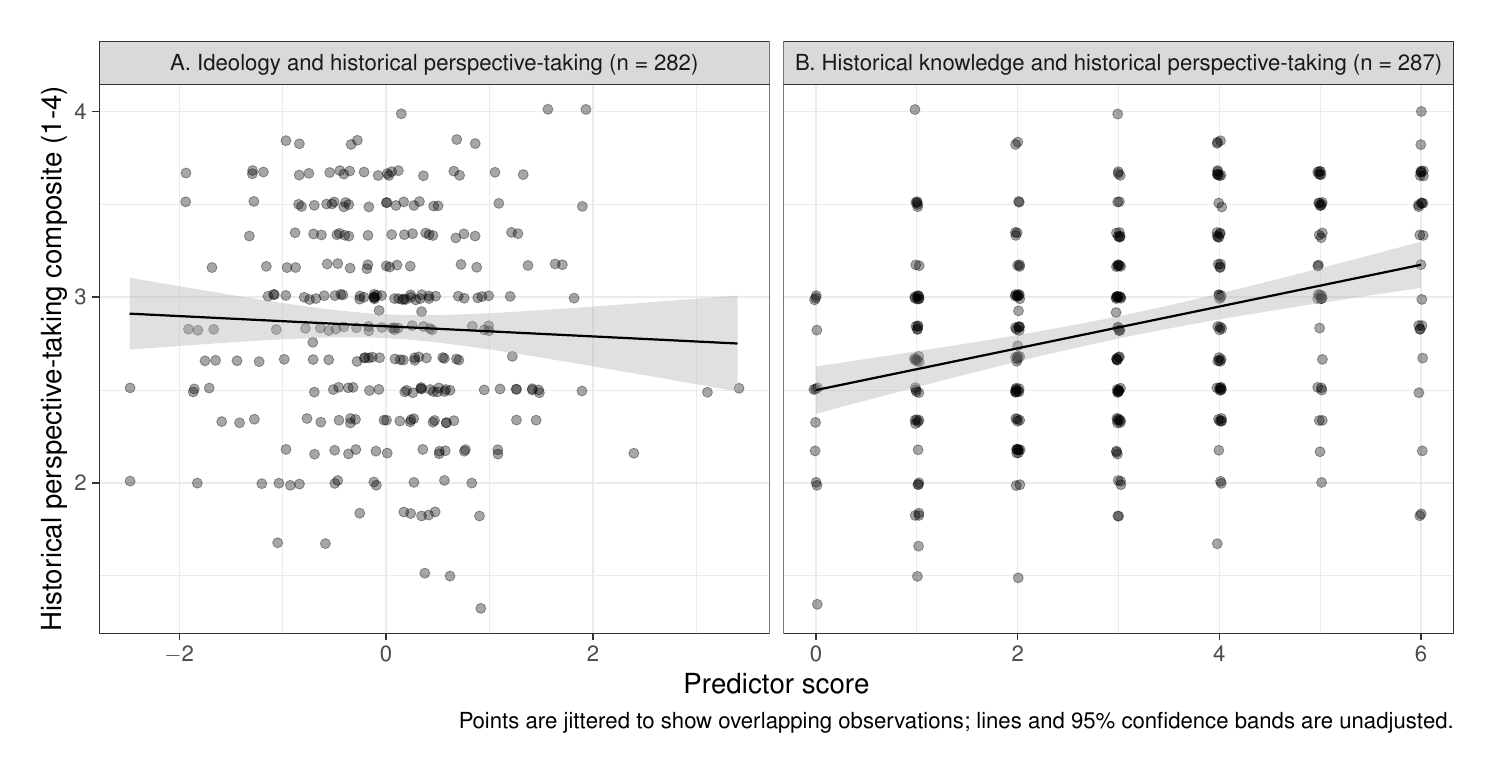
\begin{tikzpicture}[x=1pt,y=1pt,font=\fontsize{10}{12}\fontfamily{phv}\selectfont]
\definecolor{fillColor}{RGB}{255,255,255}
\path[use as bounding box,fill=fillColor,fill opacity=0.00] (0,0) rectangle (520.34,260.17);
\begin{scope}
\path[clip] (  0.00,  0.00) rectangle (520.34,260.17);
\definecolor{drawColor}{RGB}{255,255,255}
\definecolor{fillColor}{RGB}{255,255,255}

\path[draw=drawColor,line width= 0.5pt,line join=round,line cap=round,fill=fillColor] (  0.00,  0.00) rectangle (520.34,260.17);
\end{scope}
\begin{scope}
\path[clip] ( 25.80, 41.31) rectangle (268.07,239.69);
\definecolor{fillColor}{RGB}{255,255,255}

\path[fill=fillColor] ( 25.80, 41.31) rectangle (268.07,239.69);
\definecolor{drawColor}{gray}{0.92}

\path[draw=drawColor,line width= 0.3pt,line join=round] ( 25.80, 62.08) --
	(268.07, 62.08);

\path[draw=drawColor,line width= 0.3pt,line join=round] ( 25.80,129.24) --
	(268.07,129.24);

\path[draw=drawColor,line width= 0.3pt,line join=round] ( 25.80,196.39) --
	(268.07,196.39);

\path[draw=drawColor,line width= 0.3pt,line join=round] ( 92.13, 41.31) --
	( 92.13,239.69);

\path[draw=drawColor,line width= 0.3pt,line join=round] (166.90, 41.31) --
	(166.90,239.69);

\path[draw=drawColor,line width= 0.3pt,line join=round] (241.67, 41.31) --
	(241.67,239.69);

\path[draw=drawColor,line width= 0.5pt,line join=round] ( 25.80, 95.66) --
	(268.07, 95.66);

\path[draw=drawColor,line width= 0.5pt,line join=round] ( 25.80,162.81) --
	(268.07,162.81);

\path[draw=drawColor,line width= 0.5pt,line join=round] ( 25.80,229.97) --
	(268.07,229.97);

\path[draw=drawColor,line width= 0.5pt,line join=round] ( 54.75, 41.31) --
	( 54.75,239.69);

\path[draw=drawColor,line width= 0.5pt,line join=round] (129.52, 41.31) --
	(129.52,239.69);

\path[draw=drawColor,line width= 0.5pt,line join=round] (204.28, 41.31) --
	(204.28,239.69);
\definecolor{drawColor}{RGB}{0,0,0}
\definecolor{fillColor}{RGB}{0,0,0}

\path[draw=drawColor,draw opacity=0.35,line width= 0.3pt,line join=round,line cap=round,fill=fillColor,fill opacity=0.35] (112.49,118.31) circle (  1.82);

\path[draw=drawColor,draw opacity=0.35,line width= 0.3pt,line join=round,line cap=round,fill=fillColor,fill opacity=0.35] (123.50,129.06) circle (  1.82);

\path[draw=drawColor,draw opacity=0.35,line width= 0.3pt,line join=round,line cap=round,fill=fillColor,fill opacity=0.35] (176.62,118.38) circle (  1.82);

\path[draw=drawColor,draw opacity=0.35,line width= 0.3pt,line join=round,line cap=round,fill=fillColor,fill opacity=0.35] (197.45,162.44) circle (  1.82);

\path[draw=drawColor,draw opacity=0.35,line width= 0.3pt,line join=round,line cap=round,fill=fillColor,fill opacity=0.35] (142.33,157.56) circle (  1.82);

\path[draw=drawColor,draw opacity=0.35,line width= 0.3pt,line join=round,line cap=round,fill=fillColor,fill opacity=0.35] (126.91,129.46) circle (  1.82);

\path[draw=drawColor,draw opacity=0.35,line width= 0.3pt,line join=round,line cap=round,fill=fillColor,fill opacity=0.35] (138.26,173.98) circle (  1.82);

\path[draw=drawColor,draw opacity=0.35,line width= 0.3pt,line join=round,line cap=round,fill=fillColor,fill opacity=0.35] (138.47,162.72) circle (  1.82);

\path[draw=drawColor,draw opacity=0.35,line width= 0.3pt,line join=round,line cap=round,fill=fillColor,fill opacity=0.35] (146.56,128.68) circle (  1.82);

\path[draw=drawColor,draw opacity=0.35,line width= 0.3pt,line join=round,line cap=round,fill=fillColor,fill opacity=0.35] (108.02,196.43) circle (  1.82);

\path[draw=drawColor,draw opacity=0.35,line width= 0.3pt,line join=round,line cap=round,fill=fillColor,fill opacity=0.35] (163.74, 50.33) circle (  1.82);

\path[draw=drawColor,draw opacity=0.35,line width= 0.3pt,line join=round,line cap=round,fill=fillColor,fill opacity=0.35] ( 81.18,207.37) circle (  1.82);

\path[draw=drawColor,draw opacity=0.35,line width= 0.3pt,line join=round,line cap=round,fill=fillColor,fill opacity=0.35] (125.19,163.80) circle (  1.82);

\path[draw=drawColor,draw opacity=0.35,line width= 0.3pt,line join=round,line cap=round,fill=fillColor,fill opacity=0.35] (123.27,150.66) circle (  1.82);

\path[draw=drawColor,draw opacity=0.35,line width= 0.3pt,line join=round,line cap=round,fill=fillColor,fill opacity=0.35] ( 99.93,162.74) circle (  1.82);

\path[draw=drawColor,draw opacity=0.35,line width= 0.3pt,line join=round,line cap=round,fill=fillColor,fill opacity=0.35] (142.16,130.15) circle (  1.82);

\path[draw=drawColor,draw opacity=0.35,line width= 0.3pt,line join=round,line cap=round,fill=fillColor,fill opacity=0.35] (139.88,139.96) circle (  1.82);

\path[draw=drawColor,draw opacity=0.35,line width= 0.3pt,line join=round,line cap=round,fill=fillColor,fill opacity=0.35] (176.51,129.52) circle (  1.82);

\path[draw=drawColor,draw opacity=0.35,line width= 0.3pt,line join=round,line cap=round,fill=fillColor,fill opacity=0.35] (176.66,129.51) circle (  1.82);

\path[draw=drawColor,draw opacity=0.35,line width= 0.3pt,line join=round,line cap=round,fill=fillColor,fill opacity=0.35] (157.74,162.40) circle (  1.82);

\path[draw=drawColor,draw opacity=0.35,line width= 0.3pt,line join=round,line cap=round,fill=fillColor,fill opacity=0.35] (154.01,118.15) circle (  1.82);

\path[draw=drawColor,draw opacity=0.35,line width= 0.3pt,line join=round,line cap=round,fill=fillColor,fill opacity=0.35] (154.91,140.45) circle (  1.82);

\path[draw=drawColor,draw opacity=0.35,line width= 0.3pt,line join=round,line cap=round,fill=fillColor,fill opacity=0.35] (160.67,152.28) circle (  1.82);

\path[draw=drawColor,draw opacity=0.35,line width= 0.3pt,line join=round,line cap=round,fill=fillColor,fill opacity=0.35] (106.15,185.28) circle (  1.82);

\path[draw=drawColor,draw opacity=0.35,line width= 0.3pt,line join=round,line cap=round,fill=fillColor,fill opacity=0.35] (128.73,118.35) circle (  1.82);

\path[draw=drawColor,draw opacity=0.35,line width= 0.3pt,line join=round,line cap=round,fill=fillColor,fill opacity=0.35] (118.80,151.72) circle (  1.82);

\path[draw=drawColor,draw opacity=0.35,line width= 0.3pt,line join=round,line cap=round,fill=fillColor,fill opacity=0.35] (156.59,174.61) circle (  1.82);

\path[draw=drawColor,draw opacity=0.35,line width= 0.3pt,line join=round,line cap=round,fill=fillColor,fill opacity=0.35] (133.94,208.51) circle (  1.82);

\path[draw=drawColor,draw opacity=0.35,line width= 0.3pt,line join=round,line cap=round,fill=fillColor,fill opacity=0.35] (163.27, 83.71) circle (  1.82);

\path[draw=drawColor,draw opacity=0.35,line width= 0.3pt,line join=round,line cap=round,fill=fillColor,fill opacity=0.35] (114.25,207.27) circle (  1.82);

\path[draw=drawColor,draw opacity=0.35,line width= 0.3pt,line join=round,line cap=round,fill=fillColor,fill opacity=0.35] (126.64,206.74) circle (  1.82);

\path[draw=drawColor,draw opacity=0.35,line width= 0.3pt,line join=round,line cap=round,fill=fillColor,fill opacity=0.35] (184.64,129.27) circle (  1.82);

\path[draw=drawColor,draw opacity=0.35,line width= 0.3pt,line join=round,line cap=round,fill=fillColor,fill opacity=0.35] (201.72,230.62) circle (  1.82);

\path[draw=drawColor,draw opacity=0.35,line width= 0.3pt,line join=round,line cap=round,fill=fillColor,fill opacity=0.35] (126.00, 94.83) circle (  1.82);

\path[draw=drawColor,draw opacity=0.35,line width= 0.3pt,line join=round,line cap=round,fill=fillColor,fill opacity=0.35] (154.72,184.19) circle (  1.82);

\path[draw=drawColor,draw opacity=0.35,line width= 0.3pt,line join=round,line cap=round,fill=fillColor,fill opacity=0.35] (127.89,163.36) circle (  1.82);

\path[draw=drawColor,draw opacity=0.35,line width= 0.3pt,line join=round,line cap=round,fill=fillColor,fill opacity=0.35] (145.02,185.38) circle (  1.82);

\path[draw=drawColor,draw opacity=0.35,line width= 0.3pt,line join=round,line cap=round,fill=fillColor,fill opacity=0.35] ( 98.22, 95.24) circle (  1.82);

\path[draw=drawColor,draw opacity=0.35,line width= 0.3pt,line join=round,line cap=round,fill=fillColor,fill opacity=0.35] (100.35,151.54) circle (  1.82);

\path[draw=drawColor,draw opacity=0.35,line width= 0.3pt,line join=round,line cap=round,fill=fillColor,fill opacity=0.35] (132.56,151.00) circle (  1.82);

\path[draw=drawColor,draw opacity=0.35,line width= 0.3pt,line join=round,line cap=round,fill=fillColor,fill opacity=0.35] (135.38,161.92) circle (  1.82);

\path[draw=drawColor,draw opacity=0.35,line width= 0.3pt,line join=round,line cap=round,fill=fillColor,fill opacity=0.35] (118.46,118.60) circle (  1.82);

\path[draw=drawColor,draw opacity=0.35,line width= 0.3pt,line join=round,line cap=round,fill=fillColor,fill opacity=0.35] (144.90, 84.06) circle (  1.82);

\path[draw=drawColor,draw opacity=0.35,line width= 0.3pt,line join=round,line cap=round,fill=fillColor,fill opacity=0.35] (136.58,161.95) circle (  1.82);

\path[draw=drawColor,draw opacity=0.35,line width= 0.3pt,line join=round,line cap=round,fill=fillColor,fill opacity=0.35] (103.14,140.24) circle (  1.82);

\path[draw=drawColor,draw opacity=0.35,line width= 0.3pt,line join=round,line cap=round,fill=fillColor,fill opacity=0.35] (103.56,195.97) circle (  1.82);

\path[draw=drawColor,draw opacity=0.35,line width= 0.3pt,line join=round,line cap=round,fill=fillColor,fill opacity=0.35] (135.93,162.09) circle (  1.82);

\path[draw=drawColor,draw opacity=0.35,line width= 0.3pt,line join=round,line cap=round,fill=fillColor,fill opacity=0.35] (142.78,107.78) circle (  1.82);

\path[draw=drawColor,draw opacity=0.35,line width= 0.3pt,line join=round,line cap=round,fill=fillColor,fill opacity=0.35] (183.73,118.33) circle (  1.82);

\path[draw=drawColor,draw opacity=0.35,line width= 0.3pt,line join=round,line cap=round,fill=fillColor,fill opacity=0.35] (193.20,174.51) circle (  1.82);

\path[draw=drawColor,draw opacity=0.35,line width= 0.3pt,line join=round,line cap=round,fill=fillColor,fill opacity=0.35] (130.80,173.66) circle (  1.82);

\path[draw=drawColor,draw opacity=0.35,line width= 0.3pt,line join=round,line cap=round,fill=fillColor,fill opacity=0.35] (149.97,140.97) circle (  1.82);

\path[draw=drawColor,draw opacity=0.35,line width= 0.3pt,line join=round,line cap=round,fill=fillColor,fill opacity=0.35] (123.28,195.40) circle (  1.82);

\path[draw=drawColor,draw opacity=0.35,line width= 0.3pt,line join=round,line cap=round,fill=fillColor,fill opacity=0.35] (156.08,206.81) circle (  1.82);

\path[draw=drawColor,draw opacity=0.35,line width= 0.3pt,line join=round,line cap=round,fill=fillColor,fill opacity=0.35] (174.35,163.07) circle (  1.82);

\path[draw=drawColor,draw opacity=0.35,line width= 0.3pt,line join=round,line cap=round,fill=fillColor,fill opacity=0.35] (129.65,118.33) circle (  1.82);

\path[draw=drawColor,draw opacity=0.35,line width= 0.3pt,line join=round,line cap=round,fill=fillColor,fill opacity=0.35] (157.64,185.65) circle (  1.82);

\path[draw=drawColor,draw opacity=0.35,line width= 0.3pt,line join=round,line cap=round,fill=fillColor,fill opacity=0.35] (150.57,140.66) circle (  1.82);

\path[draw=drawColor,draw opacity=0.35,line width= 0.3pt,line join=round,line cap=round,fill=fillColor,fill opacity=0.35] (142.40,129.65) circle (  1.82);

\path[draw=drawColor,draw opacity=0.35,line width= 0.3pt,line join=round,line cap=round,fill=fillColor,fill opacity=0.35] (146.45,117.60) circle (  1.82);

\path[draw=drawColor,draw opacity=0.35,line width= 0.3pt,line join=round,line cap=round,fill=fillColor,fill opacity=0.35] ( 60.19,129.63) circle (  1.82);

\path[draw=drawColor,draw opacity=0.35,line width= 0.3pt,line join=round,line cap=round,fill=fillColor,fill opacity=0.35] (125.85,107.14) circle (  1.82);

\path[draw=drawColor,draw opacity=0.35,line width= 0.3pt,line join=round,line cap=round,fill=fillColor,fill opacity=0.35] (138.20,117.72) circle (  1.82);

\path[draw=drawColor,draw opacity=0.35,line width= 0.3pt,line join=round,line cap=round,fill=fillColor,fill opacity=0.35] (166.55,152.44) circle (  1.82);

\path[draw=drawColor,draw opacity=0.35,line width= 0.3pt,line join=round,line cap=round,fill=fillColor,fill opacity=0.35] (190.61,174.79) circle (  1.82);

\path[draw=drawColor,draw opacity=0.35,line width= 0.3pt,line join=round,line cap=round,fill=fillColor,fill opacity=0.35] (158.18,107.70) circle (  1.82);

\path[draw=drawColor,draw opacity=0.35,line width= 0.3pt,line join=round,line cap=round,fill=fillColor,fill opacity=0.35] (139.58, 95.85) circle (  1.82);

\path[draw=drawColor,draw opacity=0.35,line width= 0.3pt,line join=round,line cap=round,fill=fillColor,fill opacity=0.35] (174.83,186.20) circle (  1.82);

\path[draw=drawColor,draw opacity=0.35,line width= 0.3pt,line join=round,line cap=round,fill=fillColor,fill opacity=0.35] (170.26,196.68) circle (  1.82);

\path[draw=drawColor,draw opacity=0.35,line width= 0.3pt,line join=round,line cap=round,fill=fillColor,fill opacity=0.35] (133.89,151.63) circle (  1.82);

\path[draw=drawColor,draw opacity=0.35,line width= 0.3pt,line join=round,line cap=round,fill=fillColor,fill opacity=0.35] (116.02,196.24) circle (  1.82);

\path[draw=drawColor,draw opacity=0.35,line width= 0.3pt,line join=round,line cap=round,fill=fillColor,fill opacity=0.35] (111.40,151.25) circle (  1.82);

\path[draw=drawColor,draw opacity=0.35,line width= 0.3pt,line join=round,line cap=round,fill=fillColor,fill opacity=0.35] (125.32,162.66) circle (  1.82);

\path[draw=drawColor,draw opacity=0.35,line width= 0.3pt,line join=round,line cap=round,fill=fillColor,fill opacity=0.35] (155.04,219.74) circle (  1.82);

\path[draw=drawColor,draw opacity=0.35,line width= 0.3pt,line join=round,line cap=round,fill=fillColor,fill opacity=0.35] (124.55,141.13) circle (  1.82);

\path[draw=drawColor,draw opacity=0.35,line width= 0.3pt,line join=round,line cap=round,fill=fillColor,fill opacity=0.35] (161.72,218.29) circle (  1.82);

\path[draw=drawColor,draw opacity=0.35,line width= 0.3pt,line join=round,line cap=round,fill=fillColor,fill opacity=0.35] ( 85.19,208.00) circle (  1.82);

\path[draw=drawColor,draw opacity=0.35,line width= 0.3pt,line join=round,line cap=round,fill=fillColor,fill opacity=0.35] (103.58,128.48) circle (  1.82);

\path[draw=drawColor,draw opacity=0.35,line width= 0.3pt,line join=round,line cap=round,fill=fillColor,fill opacity=0.35] (162.25,173.58) circle (  1.82);

\path[draw=drawColor,draw opacity=0.35,line width= 0.3pt,line join=round,line cap=round,fill=fillColor,fill opacity=0.35] (121.99,140.96) circle (  1.82);

\path[draw=drawColor,draw opacity=0.35,line width= 0.3pt,line join=round,line cap=round,fill=fillColor,fill opacity=0.35] (150.65,128.71) circle (  1.82);

\path[draw=drawColor,draw opacity=0.35,line width= 0.3pt,line join=round,line cap=round,fill=fillColor,fill opacity=0.35] (164.96,129.27) circle (  1.82);

\path[draw=drawColor,draw opacity=0.35,line width= 0.3pt,line join=round,line cap=round,fill=fillColor,fill opacity=0.35] (175.13,141.39) circle (  1.82);

\path[draw=drawColor,draw opacity=0.35,line width= 0.3pt,line join=round,line cap=round,fill=fillColor,fill opacity=0.35] (134.47,118.02) circle (  1.82);

\path[draw=drawColor,draw opacity=0.35,line width= 0.3pt,line join=round,line cap=round,fill=fillColor,fill opacity=0.35] ( 93.71,173.48) circle (  1.82);

\path[draw=drawColor,draw opacity=0.35,line width= 0.3pt,line join=round,line cap=round,fill=fillColor,fill opacity=0.35] (113.15,163.80) circle (  1.82);

\path[draw=drawColor,draw opacity=0.35,line width= 0.3pt,line join=round,line cap=round,fill=fillColor,fill opacity=0.35] (169.95,106.08) circle (  1.82);

\path[draw=drawColor,draw opacity=0.35,line width= 0.3pt,line join=round,line cap=round,fill=fillColor,fill opacity=0.35] (135.77,140.06) circle (  1.82);

\path[draw=drawColor,draw opacity=0.35,line width= 0.3pt,line join=round,line cap=round,fill=fillColor,fill opacity=0.35] (135.92, 85.15) circle (  1.82);

\path[draw=drawColor,draw opacity=0.35,line width= 0.3pt,line join=round,line cap=round,fill=fillColor,fill opacity=0.35] (116.08,184.83) circle (  1.82);

\path[draw=drawColor,draw opacity=0.35,line width= 0.3pt,line join=round,line cap=round,fill=fillColor,fill opacity=0.35] (141.82,162.27) circle (  1.82);

\path[draw=drawColor,draw opacity=0.35,line width= 0.3pt,line join=round,line cap=round,fill=fillColor,fill opacity=0.35] (125.11,162.71) circle (  1.82);

\path[draw=drawColor,draw opacity=0.35,line width= 0.3pt,line join=round,line cap=round,fill=fillColor,fill opacity=0.35] (104.15,162.28) circle (  1.82);

\path[draw=drawColor,draw opacity=0.35,line width= 0.3pt,line join=round,line cap=round,fill=fillColor,fill opacity=0.35] (141.35,141.20) circle (  1.82);

\path[draw=drawColor,draw opacity=0.35,line width= 0.3pt,line join=round,line cap=round,fill=fillColor,fill opacity=0.35] ( 76.57,117.38) circle (  1.82);

\path[draw=drawColor,draw opacity=0.35,line width= 0.3pt,line join=round,line cap=round,fill=fillColor,fill opacity=0.35] (132.55,162.27) circle (  1.82);

\path[draw=drawColor,draw opacity=0.35,line width= 0.3pt,line join=round,line cap=round,fill=fillColor,fill opacity=0.35] (152.63,129.13) circle (  1.82);

\path[draw=drawColor,draw opacity=0.35,line width= 0.3pt,line join=round,line cap=round,fill=fillColor,fill opacity=0.35] (148.78,107.11) circle (  1.82);

\path[draw=drawColor,draw opacity=0.35,line width= 0.3pt,line join=round,line cap=round,fill=fillColor,fill opacity=0.35] (177.16,185.73) circle (  1.82);

\path[draw=drawColor,draw opacity=0.35,line width= 0.3pt,line join=round,line cap=round,fill=fillColor,fill opacity=0.35] (144.98,163.22) circle (  1.82);

\path[draw=drawColor,draw opacity=0.35,line width= 0.3pt,line join=round,line cap=round,fill=fillColor,fill opacity=0.35] ( 59.82,128.53) circle (  1.82);

\path[draw=drawColor,draw opacity=0.35,line width= 0.3pt,line join=round,line cap=round,fill=fillColor,fill opacity=0.35] (121.54,162.77) circle (  1.82);

\path[draw=drawColor,draw opacity=0.35,line width= 0.3pt,line join=round,line cap=round,fill=fillColor,fill opacity=0.35] (138.40, 84.61) circle (  1.82);

\path[draw=drawColor,draw opacity=0.35,line width= 0.3pt,line join=round,line cap=round,fill=fillColor,fill opacity=0.35] (182.36,129.72) circle (  1.82);

\path[draw=drawColor,draw opacity=0.35,line width= 0.3pt,line join=round,line cap=round,fill=fillColor,fill opacity=0.35] (168.87,207.90) circle (  1.82);

\path[draw=drawColor,draw opacity=0.35,line width= 0.3pt,line join=round,line cap=round,fill=fillColor,fill opacity=0.35] (115.93,106.15) circle (  1.82);

\path[draw=drawColor,draw opacity=0.35,line width= 0.3pt,line join=round,line cap=round,fill=fillColor,fill opacity=0.35] (152.61, 62.02) circle (  1.82);

\path[draw=drawColor,draw opacity=0.35,line width= 0.3pt,line join=round,line cap=round,fill=fillColor,fill opacity=0.35] (187.98,230.67) circle (  1.82);

\path[draw=drawColor,draw opacity=0.35,line width= 0.3pt,line join=round,line cap=round,fill=fillColor,fill opacity=0.35] (162.63,162.53) circle (  1.82);

\path[draw=drawColor,draw opacity=0.35,line width= 0.3pt,line join=round,line cap=round,fill=fillColor,fill opacity=0.35] (148.04,128.50) circle (  1.82);

\path[draw=drawColor,draw opacity=0.35,line width= 0.3pt,line join=round,line cap=round,fill=fillColor,fill opacity=0.35] (129.91,106.45) circle (  1.82);

\path[draw=drawColor,draw opacity=0.35,line width= 0.3pt,line join=round,line cap=round,fill=fillColor,fill opacity=0.35] ( 67.90,139.96) circle (  1.82);

\path[draw=drawColor,draw opacity=0.35,line width= 0.3pt,line join=round,line cap=round,fill=fillColor,fill opacity=0.35] (112.39,130.21) circle (  1.82);

\path[draw=drawColor,draw opacity=0.35,line width= 0.3pt,line join=round,line cap=round,fill=fillColor,fill opacity=0.35] (110.97, 95.49) circle (  1.82);

\path[draw=drawColor,draw opacity=0.35,line width= 0.3pt,line join=round,line cap=round,fill=fillColor,fill opacity=0.35] (140.24,161.81) circle (  1.82);

\path[draw=drawColor,draw opacity=0.35,line width= 0.3pt,line join=round,line cap=round,fill=fillColor,fill opacity=0.35] ( 75.64,139.81) circle (  1.82);

\path[draw=drawColor,draw opacity=0.35,line width= 0.3pt,line join=round,line cap=round,fill=fillColor,fill opacity=0.35] ( 64.08,139.78) circle (  1.82);

\path[draw=drawColor,draw opacity=0.35,line width= 0.3pt,line join=round,line cap=round,fill=fillColor,fill opacity=0.35] (123.18,152.22) circle (  1.82);

\path[draw=drawColor,draw opacity=0.35,line width= 0.3pt,line join=round,line cap=round,fill=fillColor,fill opacity=0.35] (160.48, 95.60) circle (  1.82);

\path[draw=drawColor,draw opacity=0.35,line width= 0.3pt,line join=round,line cap=round,fill=fillColor,fill opacity=0.35] (116.65,118.95) circle (  1.82);

\path[draw=drawColor,draw opacity=0.35,line width= 0.3pt,line join=round,line cap=round,fill=fillColor,fill opacity=0.35] (127.99,151.81) circle (  1.82);

\path[draw=drawColor,draw opacity=0.35,line width= 0.3pt,line join=round,line cap=round,fill=fillColor,fill opacity=0.35] (116.36,208.35) circle (  1.82);

\path[draw=drawColor,draw opacity=0.35,line width= 0.3pt,line join=round,line cap=round,fill=fillColor,fill opacity=0.35] (108.24,174.77) circle (  1.82);

\path[draw=drawColor,draw opacity=0.35,line width= 0.3pt,line join=round,line cap=round,fill=fillColor,fill opacity=0.35] (166.72,150.63) circle (  1.82);

\path[draw=drawColor,draw opacity=0.35,line width= 0.3pt,line join=round,line cap=round,fill=fillColor,fill opacity=0.35] (110.43,129.39) circle (  1.82);

\path[draw=drawColor,draw opacity=0.35,line width= 0.3pt,line join=round,line cap=round,fill=fillColor,fill opacity=0.35] (142.39,163.69) circle (  1.82);

\path[draw=drawColor,draw opacity=0.35,line width= 0.3pt,line join=round,line cap=round,fill=fillColor,fill opacity=0.35] ( 93.28,163.40) circle (  1.82);

\path[draw=drawColor,draw opacity=0.35,line width= 0.3pt,line join=round,line cap=round,fill=fillColor,fill opacity=0.35] (103.31,185.64) circle (  1.82);

\path[draw=drawColor,draw opacity=0.35,line width= 0.3pt,line join=round,line cap=round,fill=fillColor,fill opacity=0.35] ( 83.64,139.49) circle (  1.82);

\path[draw=drawColor,draw opacity=0.35,line width= 0.3pt,line join=round,line cap=round,fill=fillColor,fill opacity=0.35] (126.15,163.50) circle (  1.82);

\path[draw=drawColor,draw opacity=0.35,line width= 0.3pt,line join=round,line cap=round,fill=fillColor,fill opacity=0.35] (143.03,152.18) circle (  1.82);

\path[draw=drawColor,draw opacity=0.35,line width= 0.3pt,line join=round,line cap=round,fill=fillColor,fill opacity=0.35] ( 90.33, 74.05) circle (  1.82);

\path[draw=drawColor,draw opacity=0.35,line width= 0.3pt,line join=round,line cap=round,fill=fillColor,fill opacity=0.35] (113.90,163.59) circle (  1.82);

\path[draw=drawColor,draw opacity=0.35,line width= 0.3pt,line join=round,line cap=round,fill=fillColor,fill opacity=0.35] ( 98.95,195.55) circle (  1.82);

\path[draw=drawColor,draw opacity=0.35,line width= 0.3pt,line join=round,line cap=round,fill=fillColor,fill opacity=0.35] ( 98.12,206.90) circle (  1.82);

\path[draw=drawColor,draw opacity=0.35,line width= 0.3pt,line join=round,line cap=round,fill=fillColor,fill opacity=0.35] (125.08, 95.99) circle (  1.82);

\path[draw=drawColor,draw opacity=0.35,line width= 0.3pt,line join=round,line cap=round,fill=fillColor,fill opacity=0.35] (150.59, 96.57) circle (  1.82);

\path[draw=drawColor,draw opacity=0.35,line width= 0.3pt,line join=round,line cap=round,fill=fillColor,fill opacity=0.35] (155.82,140.06) circle (  1.82);

\path[draw=drawColor,draw opacity=0.35,line width= 0.3pt,line join=round,line cap=round,fill=fillColor,fill opacity=0.35] (219.04,106.39) circle (  1.82);

\path[draw=drawColor,draw opacity=0.35,line width= 0.3pt,line join=round,line cap=round,fill=fillColor,fill opacity=0.35] (107.15,163.32) circle (  1.82);

\path[draw=drawColor,draw opacity=0.35,line width= 0.3pt,line join=round,line cap=round,fill=fillColor,fill opacity=0.35] (148.57,130.00) circle (  1.82);

\path[draw=drawColor,draw opacity=0.35,line width= 0.3pt,line join=round,line cap=round,fill=fillColor,fill opacity=0.35] (130.53,206.77) circle (  1.82);

\path[draw=drawColor,draw opacity=0.35,line width= 0.3pt,line join=round,line cap=round,fill=fillColor,fill opacity=0.35] (164.98,150.98) circle (  1.82);

\path[draw=drawColor,draw opacity=0.35,line width= 0.3pt,line join=round,line cap=round,fill=fillColor,fill opacity=0.35] (129.82,196.97) circle (  1.82);

\path[draw=drawColor,draw opacity=0.35,line width= 0.3pt,line join=round,line cap=round,fill=fillColor,fill opacity=0.35] (200.44,195.58) circle (  1.82);

\path[draw=drawColor,draw opacity=0.35,line width= 0.3pt,line join=round,line cap=round,fill=fillColor,fill opacity=0.35] (161.68,184.86) circle (  1.82);

\path[draw=drawColor,draw opacity=0.35,line width= 0.3pt,line join=round,line cap=round,fill=fillColor,fill opacity=0.35] (114.60,185.14) circle (  1.82);

\path[draw=drawColor,draw opacity=0.35,line width= 0.3pt,line join=round,line cap=round,fill=fillColor,fill opacity=0.35] (184.90,128.25) circle (  1.82);

\path[draw=drawColor,draw opacity=0.35,line width= 0.3pt,line join=round,line cap=round,fill=fillColor,fill opacity=0.35] (129.95,207.44) circle (  1.82);

\path[draw=drawColor,draw opacity=0.35,line width= 0.3pt,line join=round,line cap=round,fill=fillColor,fill opacity=0.35] (180.79,174.25) circle (  1.82);

\path[draw=drawColor,draw opacity=0.35,line width= 0.3pt,line join=round,line cap=round,fill=fillColor,fill opacity=0.35] ( 89.12,163.69) circle (  1.82);

\path[draw=drawColor,draw opacity=0.35,line width= 0.3pt,line join=round,line cap=round,fill=fillColor,fill opacity=0.35] (114.87,197.01) circle (  1.82);

\path[draw=drawColor,draw opacity=0.35,line width= 0.3pt,line join=round,line cap=round,fill=fillColor,fill opacity=0.35] (141.57,197.35) circle (  1.82);

\path[draw=drawColor,draw opacity=0.35,line width= 0.3pt,line join=round,line cap=round,fill=fillColor,fill opacity=0.35] ( 86.24,173.91) circle (  1.82);

\path[draw=drawColor,draw opacity=0.35,line width= 0.3pt,line join=round,line cap=round,fill=fillColor,fill opacity=0.35] (200.29,128.89) circle (  1.82);

\path[draw=drawColor,draw opacity=0.35,line width= 0.3pt,line join=round,line cap=round,fill=fillColor,fill opacity=0.35] (179.07,207.08) circle (  1.82);

\path[draw=drawColor,draw opacity=0.35,line width= 0.3pt,line join=round,line cap=round,fill=fillColor,fill opacity=0.35] (122.94,174.51) circle (  1.82);

\path[draw=drawColor,draw opacity=0.35,line width= 0.3pt,line join=round,line cap=round,fill=fillColor,fill opacity=0.35] (133.47,174.38) circle (  1.82);

\path[draw=drawColor,draw opacity=0.35,line width= 0.3pt,line join=round,line cap=round,fill=fillColor,fill opacity=0.35] (143.00,206.66) circle (  1.82);

\path[draw=drawColor,draw opacity=0.35,line width= 0.3pt,line join=round,line cap=round,fill=fillColor,fill opacity=0.35] (143.50, 63.05) circle (  1.82);

\path[draw=drawColor,draw opacity=0.35,line width= 0.3pt,line join=round,line cap=round,fill=fillColor,fill opacity=0.35] (111.06,163.33) circle (  1.82);

\path[draw=drawColor,draw opacity=0.35,line width= 0.3pt,line join=round,line cap=round,fill=fillColor,fill opacity=0.35] ( 37.01,130.01) circle (  1.82);

\path[draw=drawColor,draw opacity=0.35,line width= 0.3pt,line join=round,line cap=round,fill=fillColor,fill opacity=0.35] (135.86,197.21) circle (  1.82);

\path[draw=drawColor,draw opacity=0.35,line width= 0.3pt,line join=round,line cap=round,fill=fillColor,fill opacity=0.35] (109.95,196.48) circle (  1.82);

\path[draw=drawColor,draw opacity=0.35,line width= 0.3pt,line join=round,line cap=round,fill=fillColor,fill opacity=0.35] (170.70,129.61) circle (  1.82);

\path[draw=drawColor,draw opacity=0.35,line width= 0.3pt,line join=round,line cap=round,fill=fillColor,fill opacity=0.35] (139.07,185.73) circle (  1.82);

\path[draw=drawColor,draw opacity=0.35,line width= 0.3pt,line join=round,line cap=round,fill=fillColor,fill opacity=0.35] (116.59,117.31) circle (  1.82);

\path[draw=drawColor,draw opacity=0.35,line width= 0.3pt,line join=round,line cap=round,fill=fillColor,fill opacity=0.35] ( 93.35,107.77) circle (  1.82);

\path[draw=drawColor,draw opacity=0.35,line width= 0.3pt,line join=round,line cap=round,fill=fillColor,fill opacity=0.35] (131.53,185.41) circle (  1.82);

\path[draw=drawColor,draw opacity=0.35,line width= 0.3pt,line join=round,line cap=round,fill=fillColor,fill opacity=0.35] (134.66,140.17) circle (  1.82);

\path[draw=drawColor,draw opacity=0.35,line width= 0.3pt,line join=round,line cap=round,fill=fillColor,fill opacity=0.35] (155.59,163.14) circle (  1.82);

\path[draw=drawColor,draw opacity=0.35,line width= 0.3pt,line join=round,line cap=round,fill=fillColor,fill opacity=0.35] (139.58,195.92) circle (  1.82);

\path[draw=drawColor,draw opacity=0.35,line width= 0.3pt,line join=round,line cap=round,fill=fillColor,fill opacity=0.35] ( 81.73,197.37) circle (  1.82);

\path[draw=drawColor,draw opacity=0.35,line width= 0.3pt,line join=round,line cap=round,fill=fillColor,fill opacity=0.35] (138.51,118.49) circle (  1.82);

\path[draw=drawColor,draw opacity=0.35,line width= 0.3pt,line join=round,line cap=round,fill=fillColor,fill opacity=0.35] (118.59,107.72) circle (  1.82);

\path[draw=drawColor,draw opacity=0.35,line width= 0.3pt,line join=round,line cap=round,fill=fillColor,fill opacity=0.35] (112.04, 96.53) circle (  1.82);

\path[draw=drawColor,draw opacity=0.35,line width= 0.3pt,line join=round,line cap=round,fill=fillColor,fill opacity=0.35] (245.63,128.42) circle (  1.82);

\path[draw=drawColor,draw opacity=0.35,line width= 0.3pt,line join=round,line cap=round,fill=fillColor,fill opacity=0.35] (148.31,195.79) circle (  1.82);

\path[draw=drawColor,draw opacity=0.35,line width= 0.3pt,line join=round,line cap=round,fill=fillColor,fill opacity=0.35] (133.08,195.92) circle (  1.82);

\path[draw=drawColor,draw opacity=0.35,line width= 0.3pt,line join=round,line cap=round,fill=fillColor,fill opacity=0.35] ( 90.79, 95.56) circle (  1.82);

\path[draw=drawColor,draw opacity=0.35,line width= 0.3pt,line join=round,line cap=round,fill=fillColor,fill opacity=0.35] (119.99, 84.72) circle (  1.82);

\path[draw=drawColor,draw opacity=0.35,line width= 0.3pt,line join=round,line cap=round,fill=fillColor,fill opacity=0.35] (129.57,174.08) circle (  1.82);

\path[draw=drawColor,draw opacity=0.35,line width= 0.3pt,line join=round,line cap=round,fill=fillColor,fill opacity=0.35] (148.68,106.20) circle (  1.82);

\path[draw=drawColor,draw opacity=0.35,line width= 0.3pt,line join=round,line cap=round,fill=fillColor,fill opacity=0.35] ( 81.28,208.55) circle (  1.82);

\path[draw=drawColor,draw opacity=0.35,line width= 0.3pt,line join=round,line cap=round,fill=fillColor,fill opacity=0.35] (135.00,229.06) circle (  1.82);

\path[draw=drawColor,draw opacity=0.35,line width= 0.3pt,line join=round,line cap=round,fill=fillColor,fill opacity=0.35] ( 96.83,173.50) circle (  1.82);

\path[draw=drawColor,draw opacity=0.35,line width= 0.3pt,line join=round,line cap=round,fill=fillColor,fill opacity=0.35] (110.92,107.45) circle (  1.82);

\path[draw=drawColor,draw opacity=0.35,line width= 0.3pt,line join=round,line cap=round,fill=fillColor,fill opacity=0.35] (146.13,150.97) circle (  1.82);

\path[draw=drawColor,draw opacity=0.35,line width= 0.3pt,line join=round,line cap=round,fill=fillColor,fill opacity=0.35] (136.11,185.37) circle (  1.82);

\path[draw=drawColor,draw opacity=0.35,line width= 0.3pt,line join=round,line cap=round,fill=fillColor,fill opacity=0.35] ( 97.89,196.34) circle (  1.82);

\path[draw=drawColor,draw opacity=0.35,line width= 0.3pt,line join=round,line cap=round,fill=fillColor,fill opacity=0.35] ( 37.02, 96.31) circle (  1.82);

\path[draw=drawColor,draw opacity=0.35,line width= 0.3pt,line join=round,line cap=round,fill=fillColor,fill opacity=0.35] ( 81.91,118.67) circle (  1.82);

\path[draw=drawColor,draw opacity=0.35,line width= 0.3pt,line join=round,line cap=round,fill=fillColor,fill opacity=0.35] (108.79,140.16) circle (  1.82);

\path[draw=drawColor,draw opacity=0.35,line width= 0.3pt,line join=round,line cap=round,fill=fillColor,fill opacity=0.35] (110.78,197.19) circle (  1.82);

\path[draw=drawColor,draw opacity=0.35,line width= 0.3pt,line join=round,line cap=round,fill=fillColor,fill opacity=0.35] ( 67.22,151.15) circle (  1.82);

\path[draw=drawColor,draw opacity=0.35,line width= 0.3pt,line join=round,line cap=round,fill=fillColor,fill opacity=0.35] (139.81,140.88) circle (  1.82);

\path[draw=drawColor,draw opacity=0.35,line width= 0.3pt,line join=round,line cap=round,fill=fillColor,fill opacity=0.35] (166.57,163.30) circle (  1.82);

\path[draw=drawColor,draw opacity=0.35,line width= 0.3pt,line join=round,line cap=round,fill=fillColor,fill opacity=0.35] ( 89.83,151.08) circle (  1.82);

\path[draw=drawColor,draw opacity=0.35,line width= 0.3pt,line join=round,line cap=round,fill=fillColor,fill opacity=0.35] (122.98,185.12) circle (  1.82);

\path[draw=drawColor,draw opacity=0.35,line width= 0.3pt,line join=round,line cap=round,fill=fillColor,fill opacity=0.35] ( 57.10,197.24) circle (  1.82);

\path[draw=drawColor,draw opacity=0.35,line width= 0.3pt,line join=round,line cap=round,fill=fillColor,fill opacity=0.35] (116.53,173.27) circle (  1.82);

\path[draw=drawColor,draw opacity=0.35,line width= 0.3pt,line join=round,line cap=round,fill=fillColor,fill opacity=0.35] (112.05,174.91) circle (  1.82);

\path[draw=drawColor,draw opacity=0.35,line width= 0.3pt,line join=round,line cap=round,fill=fillColor,fill opacity=0.35] (120.07,163.22) circle (  1.82);

\path[draw=drawColor,draw opacity=0.35,line width= 0.3pt,line join=round,line cap=round,fill=fillColor,fill opacity=0.35] (116.88,217.97) circle (  1.82);

\path[draw=drawColor,draw opacity=0.35,line width= 0.3pt,line join=round,line cap=round,fill=fillColor,fill opacity=0.35] ( 80.10,184.87) circle (  1.82);

\path[draw=drawColor,draw opacity=0.35,line width= 0.3pt,line join=round,line cap=round,fill=fillColor,fill opacity=0.35] (129.58,196.95) circle (  1.82);

\path[draw=drawColor,draw opacity=0.35,line width= 0.3pt,line join=round,line cap=round,fill=fillColor,fill opacity=0.35] (138.95,152.51) circle (  1.82);

\path[draw=drawColor,draw opacity=0.35,line width= 0.3pt,line join=round,line cap=round,fill=fillColor,fill opacity=0.35] (169.86,107.65) circle (  1.82);

\path[draw=drawColor,draw opacity=0.35,line width= 0.3pt,line join=round,line cap=round,fill=fillColor,fill opacity=0.35] ( 86.85,163.10) circle (  1.82);

\path[draw=drawColor,draw opacity=0.35,line width= 0.3pt,line join=round,line cap=round,fill=fillColor,fill opacity=0.35] (111.72,185.34) circle (  1.82);

\path[draw=drawColor,draw opacity=0.35,line width= 0.3pt,line join=round,line cap=round,fill=fillColor,fill opacity=0.35] (107.59, 73.73) circle (  1.82);

\path[draw=drawColor,draw opacity=0.35,line width= 0.3pt,line join=round,line cap=round,fill=fillColor,fill opacity=0.35] (139.53,118.87) circle (  1.82);

\path[draw=drawColor,draw opacity=0.35,line width= 0.3pt,line join=round,line cap=round,fill=fillColor,fill opacity=0.35] (119.02,139.55) circle (  1.82);

\path[draw=drawColor,draw opacity=0.35,line width= 0.3pt,line join=round,line cap=round,fill=fillColor,fill opacity=0.35] ( 84.60, 95.40) circle (  1.82);

\path[draw=drawColor,draw opacity=0.35,line width= 0.3pt,line join=round,line cap=round,fill=fillColor,fill opacity=0.35] (139.19,128.24) circle (  1.82);

\path[draw=drawColor,draw opacity=0.35,line width= 0.3pt,line join=round,line cap=round,fill=fillColor,fill opacity=0.35] (125.30,162.15) circle (  1.82);

\path[draw=drawColor,draw opacity=0.35,line width= 0.3pt,line join=round,line cap=round,fill=fillColor,fill opacity=0.35] (119.13,219.47) circle (  1.82);

\path[draw=drawColor,draw opacity=0.35,line width= 0.3pt,line join=round,line cap=round,fill=fillColor,fill opacity=0.35] (101.62,207.53) circle (  1.82);

\path[draw=drawColor,draw opacity=0.35,line width= 0.3pt,line join=round,line cap=round,fill=fillColor,fill opacity=0.35] (125.16,162.87) circle (  1.82);

\path[draw=drawColor,draw opacity=0.35,line width= 0.3pt,line join=round,line cap=round,fill=fillColor,fill opacity=0.35] (121.56,207.99) circle (  1.82);

\path[draw=drawColor,draw opacity=0.35,line width= 0.3pt,line join=round,line cap=round,fill=fillColor,fill opacity=0.35] (114.24,195.43) circle (  1.82);

\path[draw=drawColor,draw opacity=0.35,line width= 0.3pt,line join=round,line cap=round,fill=fillColor,fill opacity=0.35] (131.53,208.13) circle (  1.82);

\path[draw=drawColor,draw opacity=0.35,line width= 0.3pt,line join=round,line cap=round,fill=fillColor,fill opacity=0.35] ( 57.20,207.64) circle (  1.82);

\path[draw=drawColor,draw opacity=0.35,line width= 0.3pt,line join=round,line cap=round,fill=fillColor,fill opacity=0.35] (109.13,207.82) circle (  1.82);

\path[draw=drawColor,draw opacity=0.35,line width= 0.3pt,line join=round,line cap=round,fill=fillColor,fill opacity=0.35] ( 96.62,186.07) circle (  1.82);

\path[draw=drawColor,draw opacity=0.35,line width= 0.3pt,line join=round,line cap=round,fill=fillColor,fill opacity=0.35] ( 61.50,150.82) circle (  1.82);

\path[draw=drawColor,draw opacity=0.35,line width= 0.3pt,line join=round,line cap=round,fill=fillColor,fill opacity=0.35] (157.79,107.11) circle (  1.82);

\path[draw=drawColor,draw opacity=0.35,line width= 0.3pt,line join=round,line cap=round,fill=fillColor,fill opacity=0.35] (145.03,162.29) circle (  1.82);

\path[draw=drawColor,draw opacity=0.35,line width= 0.3pt,line join=round,line cap=round,fill=fillColor,fill opacity=0.35] (127.17,140.90) circle (  1.82);

\path[draw=drawColor,draw opacity=0.35,line width= 0.3pt,line join=round,line cap=round,fill=fillColor,fill opacity=0.35] (257.06,129.86) circle (  1.82);

\path[draw=drawColor,draw opacity=0.35,line width= 0.3pt,line join=round,line cap=round,fill=fillColor,fill opacity=0.35] (108.81,150.74) circle (  1.82);

\path[draw=drawColor,draw opacity=0.35,line width= 0.3pt,line join=round,line cap=round,fill=fillColor,fill opacity=0.35] (134.05,162.27) circle (  1.82);

\path[draw=drawColor,draw opacity=0.35,line width= 0.3pt,line join=round,line cap=round,fill=fillColor,fill opacity=0.35] (150.90,107.28) circle (  1.82);

\path[draw=drawColor,draw opacity=0.35,line width= 0.3pt,line join=round,line cap=round,fill=fillColor,fill opacity=0.35] (105.74,151.64) circle (  1.82);

\path[draw=drawColor,draw opacity=0.35,line width= 0.3pt,line join=round,line cap=round,fill=fillColor,fill opacity=0.35] (101.86,161.93) circle (  1.82);

\path[draw=drawColor,draw opacity=0.35,line width= 0.3pt,line join=round,line cap=round,fill=fillColor,fill opacity=0.35] (143.82,185.97) circle (  1.82);

\path[draw=drawColor,draw opacity=0.35,line width= 0.3pt,line join=round,line cap=round,fill=fillColor,fill opacity=0.35] (151.23,117.43) circle (  1.82);

\path[draw=drawColor,draw opacity=0.35,line width= 0.3pt,line join=round,line cap=round,fill=fillColor,fill opacity=0.35] (147.05,118.24) circle (  1.82);

\path[draw=drawColor,draw opacity=0.35,line width= 0.3pt,line join=round,line cap=round,fill=fillColor,fill opacity=0.35] (117.57,130.19) circle (  1.82);

\path[draw=drawColor,draw opacity=0.35,line width= 0.3pt,line join=round,line cap=round,fill=fillColor,fill opacity=0.35] ( 94.93, 94.80) circle (  1.82);

\path[draw=drawColor,draw opacity=0.35,line width= 0.3pt,line join=round,line cap=round,fill=fillColor,fill opacity=0.35] (145.44,129.43) circle (  1.82);

\path[draw=drawColor,draw opacity=0.35,line width= 0.3pt,line join=round,line cap=round,fill=fillColor,fill opacity=0.35] (123.27,140.82) circle (  1.82);

\path[draw=drawColor,draw opacity=0.35,line width= 0.3pt,line join=round,line cap=round,fill=fillColor,fill opacity=0.35] (114.21,152.03) circle (  1.82);

\path[draw=drawColor,draw opacity=0.35,line width= 0.3pt,line join=round,line cap=round,fill=fillColor,fill opacity=0.35] ( 66.60,173.49) circle (  1.82);

\path[draw=drawColor,draw opacity=0.35,line width= 0.3pt,line join=round,line cap=round,fill=fillColor,fill opacity=0.35] (142.34, 83.73) circle (  1.82);

\path[draw=drawColor,draw opacity=0.35,line width= 0.3pt,line join=round,line cap=round,fill=fillColor,fill opacity=0.35] (119.99,162.07) circle (  1.82);

\path[draw=drawColor,draw opacity=0.35,line width= 0.3pt,line join=round,line cap=round,fill=fillColor,fill opacity=0.35] ( 65.62,129.94) circle (  1.82);

\path[draw=drawColor,draw opacity=0.35,line width= 0.3pt,line join=round,line cap=round,fill=fillColor,fill opacity=0.35] (136.26,128.56) circle (  1.82);

\path[draw=drawColor,draw opacity=0.35,line width= 0.3pt,line join=round,line cap=round,fill=fillColor,fill opacity=0.35] (122.56,173.06) circle (  1.82);

\path[draw=drawColor,draw opacity=0.35,line width= 0.3pt,line join=round,line cap=round,fill=fillColor,fill opacity=0.35] (121.59,140.78) circle (  1.82);

\path[draw=drawColor,draw opacity=0.35,line width= 0.3pt,line join=round,line cap=round,fill=fillColor,fill opacity=0.35] (146.45,185.07) circle (  1.82);

\path[draw=drawColor,draw opacity=0.35,line width= 0.3pt,line join=round,line cap=round,fill=fillColor,fill opacity=0.35] (141.99,129.72) circle (  1.82);

\path[draw=drawColor,draw opacity=0.35,line width= 0.3pt,line join=round,line cap=round,fill=fillColor,fill opacity=0.35] (153.99,208.32) circle (  1.82);

\path[draw=drawColor,draw opacity=0.35,line width= 0.3pt,line join=round,line cap=round,fill=fillColor,fill opacity=0.35] (182.33,129.25) circle (  1.82);

\path[draw=drawColor,draw opacity=0.35,line width= 0.3pt,line join=round,line cap=round,fill=fillColor,fill opacity=0.35] (136.95,129.13) circle (  1.82);

\path[draw=drawColor,draw opacity=0.35,line width= 0.3pt,line join=round,line cap=round,fill=fillColor,fill opacity=0.35] (151.30,117.40) circle (  1.82);

\path[draw=drawColor,draw opacity=0.35,line width= 0.3pt,line join=round,line cap=round,fill=fillColor,fill opacity=0.35] (151.07,129.44) circle (  1.82);

\path[draw=drawColor,draw opacity=0.35,line width= 0.3pt,line join=round,line cap=round,fill=fillColor,fill opacity=0.35] (103.03,146.47) circle (  1.82);

\path[draw=drawColor,draw opacity=0.35,line width= 0.3pt,line join=round,line cap=round,fill=fillColor,fill opacity=0.35] ( 92.71,140.32) circle (  1.82);

\path[draw=drawColor,draw opacity=0.35,line width= 0.3pt,line join=round,line cap=round,fill=fillColor,fill opacity=0.35] (127.00,157.99) circle (  1.82);

\path[draw=drawColor,draw opacity=0.35,line width= 0.3pt,line join=round,line cap=round,fill=fillColor,fill opacity=0.35] (147.23, 85.20) circle (  1.82);

\path[draw=drawColor,draw opacity=0.35,line width= 0.3pt,line join=round,line cap=round,fill=fillColor,fill opacity=0.35] ( 70.11,117.83) circle (  1.82);

\path[draw=drawColor,draw opacity=0.35,line width= 0.3pt,line join=round,line cap=round,fill=fillColor,fill opacity=0.35] (146.72,195.70) circle (  1.82);

\path[draw=drawColor,draw opacity=0.35,line width= 0.3pt,line join=round,line cap=round,fill=fillColor,fill opacity=0.35] (145.31,151.50) circle (  1.82);

\path[draw=drawColor,draw opacity=0.35,line width= 0.3pt,line join=round,line cap=round,fill=fillColor,fill opacity=0.35] (147.41,163.16) circle (  1.82);

\path[draw=drawColor,draw opacity=0.35,line width= 0.3pt,line join=round,line cap=round,fill=fillColor,fill opacity=0.35] (132.71,140.46) circle (  1.82);

\path[draw=drawColor,draw opacity=0.35,line width= 0.3pt,line join=round,line cap=round,fill=fillColor,fill opacity=0.35] (103.66,106.04) circle (  1.82);

\path[draw=drawColor,draw opacity=0.35,line width= 0.3pt,line join=round,line cap=round,fill=fillColor,fill opacity=0.35] (112.79,208.51) circle (  1.82);

\path[draw=drawColor,draw opacity=0.35,line width= 0.3pt,line join=round,line cap=round,fill=fillColor,fill opacity=0.35] (112.66,185.83) circle (  1.82);

\path[draw=drawColor,draw opacity=0.35,line width= 0.3pt,line join=round,line cap=round,fill=fillColor,fill opacity=0.35] ( 98.18,218.21) circle (  1.82);

\path[draw=drawColor,draw opacity=0.35,line width= 0.3pt,line join=round,line cap=round,fill=fillColor,fill opacity=0.35] ( 88.90,163.77) circle (  1.82);

\path[draw=drawColor,draw opacity=0.35,line width= 0.3pt,line join=round,line cap=round,fill=fillColor,fill opacity=0.35] (100.94,118.94) circle (  1.82);

\path[draw=drawColor,draw opacity=0.35,line width= 0.3pt,line join=round,line cap=round,fill=fillColor,fill opacity=0.35] ( 93.32,219.34) circle (  1.82);

\path[draw=drawColor,draw opacity=0.35,line width= 0.3pt,line join=round,line cap=round,fill=fillColor,fill opacity=0.35] (105.92,117.61) circle (  1.82);

\path[draw=drawColor,draw opacity=0.35,line width= 0.3pt,line join=round,line cap=round,fill=fillColor,fill opacity=0.35] ( 61.30, 95.60) circle (  1.82);

\path[draw=drawColor,draw opacity=0.35,line width= 0.3pt,line join=round,line cap=round,fill=fillColor,fill opacity=0.35] (144.11,140.81) circle (  1.82);

\path[draw=drawColor,draw opacity=0.35,line width= 0.3pt,line join=round,line cap=round,fill=fillColor,fill opacity=0.35] (138.38,163.62) circle (  1.82);

\path[draw=drawColor,draw opacity=0.35,line width= 0.3pt,line join=round,line cap=round,fill=fillColor,fill opacity=0.35] (115.87,130.03) circle (  1.82);

\path[draw=drawColor,draw opacity=0.35,line width= 0.3pt,line join=round,line cap=round,fill=fillColor,fill opacity=0.35] (131.66,151.67) circle (  1.82);

\path[draw=drawColor,draw opacity=0.35,line width= 0.3pt,line join=round,line cap=round,fill=fillColor,fill opacity=0.35] (164.16,163.01) circle (  1.82);

\path[draw=drawColor,draw opacity=0.35,line width= 0.3pt,line join=round,line cap=round,fill=fillColor,fill opacity=0.35] (132.61,151.73) circle (  1.82);

\path[draw=drawColor,draw opacity=0.35,line width= 0.3pt,line join=round,line cap=round,fill=fillColor,fill opacity=0.35] ( 58.09,151.21) circle (  1.82);
\definecolor{fillColor}{RGB}{179,179,179}

\path[fill=fillColor,fill opacity=0.40] ( 36.81,169.84) --
	( 39.59,169.35) --
	( 42.37,168.87) --
	( 45.15,168.39) --
	( 47.93,167.91) --
	( 50.71,167.43) --
	( 53.50,166.96) --
	( 56.28,166.48) --
	( 59.06,166.01) --
	( 61.84,165.54) --
	( 64.62,165.08) --
	( 67.40,164.61) --
	( 70.18,164.15) --
	( 72.96,163.69) --
	( 75.74,163.24) --
	( 78.52,162.79) --
	( 81.30,162.35) --
	( 84.09,161.91) --
	( 86.87,161.48) --
	( 89.65,161.05) --
	( 92.43,160.63) --
	( 95.21,160.22) --
	( 97.99,159.83) --
	(100.77,159.44) --
	(103.55,159.07) --
	(106.33,158.71) --
	(109.11,158.37) --
	(111.89,158.05) --
	(114.67,157.75) --
	(117.46,157.47) --
	(120.24,157.22) --
	(123.02,157.00) --
	(125.80,156.80) --
	(128.58,156.64) --
	(131.36,156.51) --
	(134.14,156.41) --
	(136.92,156.34) --
	(139.70,156.30) --
	(142.48,156.28) --
	(145.26,156.29) --
	(148.05,156.33) --
	(150.83,156.38) --
	(153.61,156.46) --
	(156.39,156.55) --
	(159.17,156.65) --
	(161.95,156.77) --
	(164.73,156.90) --
	(167.51,157.04) --
	(170.29,157.18) --
	(173.07,157.34) --
	(175.85,157.50) --
	(178.63,157.67) --
	(181.42,157.84) --
	(184.20,158.02) --
	(186.98,158.20) --
	(189.76,158.38) --
	(192.54,158.57) --
	(195.32,158.76) --
	(198.10,158.96) --
	(200.88,159.16) --
	(203.66,159.35) --
	(206.44,159.56) --
	(209.22,159.76) --
	(212.01,159.96) --
	(214.79,160.17) --
	(217.57,160.38) --
	(220.35,160.59) --
	(223.13,160.80) --
	(225.91,161.01) --
	(228.69,161.22) --
	(231.47,161.44) --
	(234.25,161.65) --
	(237.03,161.87) --
	(239.81,162.08) --
	(242.59,162.30) --
	(245.38,162.52) --
	(248.16,162.73) --
	(250.94,162.95) --
	(253.72,163.17) --
	(256.50,163.39) --
	(256.50,128.69) --
	(253.72,129.18) --
	(250.94,129.67) --
	(248.16,130.16) --
	(245.38,130.66) --
	(242.59,131.15) --
	(239.81,131.64) --
	(237.03,132.13) --
	(234.25,132.61) --
	(231.47,133.10) --
	(228.69,133.59) --
	(225.91,134.07) --
	(223.13,134.56) --
	(220.35,135.04) --
	(217.57,135.52) --
	(214.79,136.01) --
	(212.01,136.48) --
	(209.22,136.96) --
	(206.44,137.44) --
	(203.66,137.91) --
	(200.88,138.39) --
	(198.10,138.86) --
	(195.32,139.32) --
	(192.54,139.79) --
	(189.76,140.25) --
	(186.98,140.71) --
	(184.20,141.16) --
	(181.42,141.61) --
	(178.63,142.06) --
	(175.85,142.50) --
	(173.07,142.94) --
	(170.29,143.36) --
	(167.51,143.78) --
	(164.73,144.19) --
	(161.95,144.60) --
	(159.17,144.99) --
	(156.39,145.36) --
	(153.61,145.73) --
	(150.83,146.07) --
	(148.05,146.40) --
	(145.26,146.71) --
	(142.48,146.99) --
	(139.70,147.25) --
	(136.92,147.49) --
	(134.14,147.69) --
	(131.36,147.86) --
	(128.58,148.00) --
	(125.80,148.11) --
	(123.02,148.19) --
	(120.24,148.24) --
	(117.46,148.27) --
	(114.67,148.26) --
	(111.89,148.24) --
	(109.11,148.19) --
	(106.33,148.12) --
	(103.55,148.03) --
	(100.77,147.93) --
	( 97.99,147.82) --
	( 95.21,147.70) --
	( 92.43,147.56) --
	( 89.65,147.42) --
	( 86.87,147.26) --
	( 84.09,147.10) --
	( 81.30,146.94) --
	( 78.52,146.77) --
	( 75.74,146.59) --
	( 72.96,146.41) --
	( 70.18,146.23) --
	( 67.40,146.04) --
	( 64.62,145.85) --
	( 61.84,145.66) --
	( 59.06,145.46) --
	( 56.28,145.26) --
	( 53.50,145.06) --
	( 50.71,144.86) --
	( 47.93,144.65) --
	( 45.15,144.45) --
	( 42.37,144.24) --
	( 39.59,144.03) --
	( 36.81,143.82) --
	cycle;

\path[] ( 36.81,169.84) --
	( 39.59,169.35) --
	( 42.37,168.87) --
	( 45.15,168.39) --
	( 47.93,167.91) --
	( 50.71,167.43) --
	( 53.50,166.96) --
	( 56.28,166.48) --
	( 59.06,166.01) --
	( 61.84,165.54) --
	( 64.62,165.08) --
	( 67.40,164.61) --
	( 70.18,164.15) --
	( 72.96,163.69) --
	( 75.74,163.24) --
	( 78.52,162.79) --
	( 81.30,162.35) --
	( 84.09,161.91) --
	( 86.87,161.48) --
	( 89.65,161.05) --
	( 92.43,160.63) --
	( 95.21,160.22) --
	( 97.99,159.83) --
	(100.77,159.44) --
	(103.55,159.07) --
	(106.33,158.71) --
	(109.11,158.37) --
	(111.89,158.05) --
	(114.67,157.75) --
	(117.46,157.47) --
	(120.24,157.22) --
	(123.02,157.00) --
	(125.80,156.80) --
	(128.58,156.64) --
	(131.36,156.51) --
	(134.14,156.41) --
	(136.92,156.34) --
	(139.70,156.30) --
	(142.48,156.28) --
	(145.26,156.29) --
	(148.05,156.33) --
	(150.83,156.38) --
	(153.61,156.46) --
	(156.39,156.55) --
	(159.17,156.65) --
	(161.95,156.77) --
	(164.73,156.90) --
	(167.51,157.04) --
	(170.29,157.18) --
	(173.07,157.34) --
	(175.85,157.50) --
	(178.63,157.67) --
	(181.42,157.84) --
	(184.20,158.02) --
	(186.98,158.20) --
	(189.76,158.38) --
	(192.54,158.57) --
	(195.32,158.76) --
	(198.10,158.96) --
	(200.88,159.16) --
	(203.66,159.35) --
	(206.44,159.56) --
	(209.22,159.76) --
	(212.01,159.96) --
	(214.79,160.17) --
	(217.57,160.38) --
	(220.35,160.59) --
	(223.13,160.80) --
	(225.91,161.01) --
	(228.69,161.22) --
	(231.47,161.44) --
	(234.25,161.65) --
	(237.03,161.87) --
	(239.81,162.08) --
	(242.59,162.30) --
	(245.38,162.52) --
	(248.16,162.73) --
	(250.94,162.95) --
	(253.72,163.17) --
	(256.50,163.39);

\path[] (256.50,128.69) --
	(253.72,129.18) --
	(250.94,129.67) --
	(248.16,130.16) --
	(245.38,130.66) --
	(242.59,131.15) --
	(239.81,131.64) --
	(237.03,132.13) --
	(234.25,132.61) --
	(231.47,133.10) --
	(228.69,133.59) --
	(225.91,134.07) --
	(223.13,134.56) --
	(220.35,135.04) --
	(217.57,135.52) --
	(214.79,136.01) --
	(212.01,136.48) --
	(209.22,136.96) --
	(206.44,137.44) --
	(203.66,137.91) --
	(200.88,138.39) --
	(198.10,138.86) --
	(195.32,139.32) --
	(192.54,139.79) --
	(189.76,140.25) --
	(186.98,140.71) --
	(184.20,141.16) --
	(181.42,141.61) --
	(178.63,142.06) --
	(175.85,142.50) --
	(173.07,142.94) --
	(170.29,143.36) --
	(167.51,143.78) --
	(164.73,144.19) --
	(161.95,144.60) --
	(159.17,144.99) --
	(156.39,145.36) --
	(153.61,145.73) --
	(150.83,146.07) --
	(148.05,146.40) --
	(145.26,146.71) --
	(142.48,146.99) --
	(139.70,147.25) --
	(136.92,147.49) --
	(134.14,147.69) --
	(131.36,147.86) --
	(128.58,148.00) --
	(125.80,148.11) --
	(123.02,148.19) --
	(120.24,148.24) --
	(117.46,148.27) --
	(114.67,148.26) --
	(111.89,148.24) --
	(109.11,148.19) --
	(106.33,148.12) --
	(103.55,148.03) --
	(100.77,147.93) --
	( 97.99,147.82) --
	( 95.21,147.70) --
	( 92.43,147.56) --
	( 89.65,147.42) --
	( 86.87,147.26) --
	( 84.09,147.10) --
	( 81.30,146.94) --
	( 78.52,146.77) --
	( 75.74,146.59) --
	( 72.96,146.41) --
	( 70.18,146.23) --
	( 67.40,146.04) --
	( 64.62,145.85) --
	( 61.84,145.66) --
	( 59.06,145.46) --
	( 56.28,145.26) --
	( 53.50,145.06) --
	( 50.71,144.86) --
	( 47.93,144.65) --
	( 45.15,144.45) --
	( 42.37,144.24) --
	( 39.59,144.03) --
	( 36.81,143.82);
\definecolor{drawColor}{RGB}{0,0,0}

\path[draw=drawColor,line width= 0.8pt,line join=round] ( 36.81,156.83) --
	( 39.59,156.69) --
	( 42.37,156.56) --
	( 45.15,156.42) --
	( 47.93,156.28) --
	( 50.71,156.15) --
	( 53.50,156.01) --
	( 56.28,155.87) --
	( 59.06,155.74) --
	( 61.84,155.60) --
	( 64.62,155.46) --
	( 67.40,155.33) --
	( 70.18,155.19) --
	( 72.96,155.05) --
	( 75.74,154.92) --
	( 78.52,154.78) --
	( 81.30,154.64) --
	( 84.09,154.51) --
	( 86.87,154.37) --
	( 89.65,154.23) --
	( 92.43,154.10) --
	( 95.21,153.96) --
	( 97.99,153.82) --
	(100.77,153.69) --
	(103.55,153.55) --
	(106.33,153.41) --
	(109.11,153.28) --
	(111.89,153.14) --
	(114.67,153.00) --
	(117.46,152.87) --
	(120.24,152.73) --
	(123.02,152.59) --
	(125.80,152.46) --
	(128.58,152.32) --
	(131.36,152.18) --
	(134.14,152.05) --
	(136.92,151.91) --
	(139.70,151.78) --
	(142.48,151.64) --
	(145.26,151.50) --
	(148.05,151.37) --
	(150.83,151.23) --
	(153.61,151.09) --
	(156.39,150.96) --
	(159.17,150.82) --
	(161.95,150.68) --
	(164.73,150.55) --
	(167.51,150.41) --
	(170.29,150.27) --
	(173.07,150.14) --
	(175.85,150.00) --
	(178.63,149.86) --
	(181.42,149.73) --
	(184.20,149.59) --
	(186.98,149.45) --
	(189.76,149.32) --
	(192.54,149.18) --
	(195.32,149.04) --
	(198.10,148.91) --
	(200.88,148.77) --
	(203.66,148.63) --
	(206.44,148.50) --
	(209.22,148.36) --
	(212.01,148.22) --
	(214.79,148.09) --
	(217.57,147.95) --
	(220.35,147.81) --
	(223.13,147.68) --
	(225.91,147.54) --
	(228.69,147.41) --
	(231.47,147.27) --
	(234.25,147.13) --
	(237.03,147.00) --
	(239.81,146.86) --
	(242.59,146.72) --
	(245.38,146.59) --
	(248.16,146.45) --
	(250.94,146.31) --
	(253.72,146.18) --
	(256.50,146.04);
\definecolor{drawColor}{gray}{0.20}

\path[draw=drawColor,line width= 0.5pt,line join=round,line cap=round] ( 25.80, 41.31) rectangle (268.07,239.69);
\end{scope}
\begin{scope}
\path[clip] (273.07, 41.31) rectangle (515.34,239.69);
\definecolor{fillColor}{RGB}{255,255,255}

\path[fill=fillColor] (273.07, 41.31) rectangle (515.34,239.69);
\definecolor{drawColor}{gray}{0.92}

\path[draw=drawColor,line width= 0.3pt,line join=round] (273.07, 62.08) --
	(515.34, 62.08);

\path[draw=drawColor,line width= 0.3pt,line join=round] (273.07,129.24) --
	(515.34,129.24);

\path[draw=drawColor,line width= 0.3pt,line join=round] (273.07,196.39) --
	(515.34,196.39);

\path[draw=drawColor,line width= 0.3pt,line join=round] (321.31, 41.31) --
	(321.31,239.69);

\path[draw=drawColor,line width= 0.3pt,line join=round] (394.17, 41.31) --
	(394.17,239.69);

\path[draw=drawColor,line width= 0.3pt,line join=round] (467.04, 41.31) --
	(467.04,239.69);

\path[draw=drawColor,line width= 0.5pt,line join=round] (273.07, 95.66) --
	(515.34, 95.66);

\path[draw=drawColor,line width= 0.5pt,line join=round] (273.07,162.81) --
	(515.34,162.81);

\path[draw=drawColor,line width= 0.5pt,line join=round] (273.07,229.97) --
	(515.34,229.97);

\path[draw=drawColor,line width= 0.5pt,line join=round] (284.87, 41.31) --
	(284.87,239.69);

\path[draw=drawColor,line width= 0.5pt,line join=round] (357.74, 41.31) --
	(357.74,239.69);

\path[draw=drawColor,line width= 0.5pt,line join=round] (430.61, 41.31) --
	(430.61,239.69);

\path[draw=drawColor,line width= 0.5pt,line join=round] (503.47, 41.31) --
	(503.47,239.69);
\definecolor{drawColor}{RGB}{0,0,0}
\definecolor{fillColor}{RGB}{0,0,0}

\path[draw=drawColor,draw opacity=0.35,line width= 0.3pt,line join=round,line cap=round,fill=fillColor,fill opacity=0.35] (467.81,118.27) circle (  1.82);

\path[draw=drawColor,draw opacity=0.35,line width= 0.3pt,line join=round,line cap=round,fill=fillColor,fill opacity=0.35] (357.07,129.21) circle (  1.82);

\path[draw=drawColor,draw opacity=0.35,line width= 0.3pt,line join=round,line cap=round,fill=fillColor,fill opacity=0.35] (431.42,117.95) circle (  1.82);

\path[draw=drawColor,draw opacity=0.35,line width= 0.3pt,line join=round,line cap=round,fill=fillColor,fill opacity=0.35] (393.39,162.26) circle (  1.82);

\path[draw=drawColor,draw opacity=0.35,line width= 0.3pt,line join=round,line cap=round,fill=fillColor,fill opacity=0.35] (393.30,157.25) circle (  1.82);

\path[draw=drawColor,draw opacity=0.35,line width= 0.3pt,line join=round,line cap=round,fill=fillColor,fill opacity=0.35] (321.12,128.67) circle (  1.82);

\path[draw=drawColor,draw opacity=0.35,line width= 0.3pt,line join=round,line cap=round,fill=fillColor,fill opacity=0.35] (393.40,173.80) circle (  1.82);

\path[draw=drawColor,draw opacity=0.35,line width= 0.3pt,line join=round,line cap=round,fill=fillColor,fill opacity=0.35] (466.42,163.80) circle (  1.82);

\path[draw=drawColor,draw opacity=0.35,line width= 0.3pt,line join=round,line cap=round,fill=fillColor,fill opacity=0.35] (322.03,128.28) circle (  1.82);

\path[draw=drawColor,draw opacity=0.35,line width= 0.3pt,line join=round,line cap=round,fill=fillColor,fill opacity=0.35] (467.54,196.32) circle (  1.82);

\path[draw=drawColor,draw opacity=0.35,line width= 0.3pt,line join=round,line cap=round,fill=fillColor,fill opacity=0.35] (285.33, 51.81) circle (  1.82);

\path[draw=drawColor,draw opacity=0.35,line width= 0.3pt,line join=round,line cap=round,fill=fillColor,fill opacity=0.35] (430.10,207.11) circle (  1.82);

\path[draw=drawColor,draw opacity=0.35,line width= 0.3pt,line join=round,line cap=round,fill=fillColor,fill opacity=0.35] (357.90,163.10) circle (  1.82);

\path[draw=drawColor,draw opacity=0.35,line width= 0.3pt,line join=round,line cap=round,fill=fillColor,fill opacity=0.35] (394.11,151.90) circle (  1.82);

\path[draw=drawColor,draw opacity=0.35,line width= 0.3pt,line join=round,line cap=round,fill=fillColor,fill opacity=0.35] (467.78,162.40) circle (  1.82);

\path[draw=drawColor,draw opacity=0.35,line width= 0.3pt,line join=round,line cap=round,fill=fillColor,fill opacity=0.35] (320.93,129.35) circle (  1.82);

\path[draw=drawColor,draw opacity=0.35,line width= 0.3pt,line join=round,line cap=round,fill=fillColor,fill opacity=0.35] (357.67,140.45) circle (  1.82);

\path[draw=drawColor,draw opacity=0.35,line width= 0.3pt,line join=round,line cap=round,fill=fillColor,fill opacity=0.35] (394.89,129.89) circle (  1.82);

\path[draw=drawColor,draw opacity=0.35,line width= 0.3pt,line join=round,line cap=round,fill=fillColor,fill opacity=0.35] (394.27,129.32) circle (  1.82);

\path[draw=drawColor,draw opacity=0.35,line width= 0.3pt,line join=round,line cap=round,fill=fillColor,fill opacity=0.35] (393.61,163.12) circle (  1.82);

\path[draw=drawColor,draw opacity=0.35,line width= 0.3pt,line join=round,line cap=round,fill=fillColor,fill opacity=0.35] (431.30,118.14) circle (  1.82);

\path[draw=drawColor,draw opacity=0.35,line width= 0.3pt,line join=round,line cap=round,fill=fillColor,fill opacity=0.35] (394.20,141.03) circle (  1.82);

\path[draw=drawColor,draw opacity=0.35,line width= 0.3pt,line join=round,line cap=round,fill=fillColor,fill opacity=0.35] (502.64,152.55) circle (  1.82);

\path[draw=drawColor,draw opacity=0.35,line width= 0.3pt,line join=round,line cap=round,fill=fillColor,fill opacity=0.35] (430.11,184.44) circle (  1.82);

\path[draw=drawColor,draw opacity=0.35,line width= 0.3pt,line join=round,line cap=round,fill=fillColor,fill opacity=0.35] (321.74,117.73) circle (  1.82);

\path[draw=drawColor,draw opacity=0.35,line width= 0.3pt,line join=round,line cap=round,fill=fillColor,fill opacity=0.35] (394.63,150.78) circle (  1.82);

\path[draw=drawColor,draw opacity=0.35,line width= 0.3pt,line join=round,line cap=round,fill=fillColor,fill opacity=0.35] (466.18,174.03) circle (  1.82);

\path[draw=drawColor,draw opacity=0.35,line width= 0.3pt,line join=round,line cap=round,fill=fillColor,fill opacity=0.35] (466.79,208.24) circle (  1.82);

\path[draw=drawColor,draw opacity=0.35,line width= 0.3pt,line join=round,line cap=round,fill=fillColor,fill opacity=0.35] (394.23, 83.63) circle (  1.82);

\path[draw=drawColor,draw opacity=0.35,line width= 0.3pt,line join=round,line cap=round,fill=fillColor,fill opacity=0.35] (504.33,206.58) circle (  1.82);

\path[draw=drawColor,draw opacity=0.35,line width= 0.3pt,line join=round,line cap=round,fill=fillColor,fill opacity=0.35] (394.10,208.13) circle (  1.82);

\path[draw=drawColor,draw opacity=0.35,line width= 0.3pt,line join=round,line cap=round,fill=fillColor,fill opacity=0.35] (466.72,118.23) circle (  1.82);

\path[draw=drawColor,draw opacity=0.35,line width= 0.3pt,line join=round,line cap=round,fill=fillColor,fill opacity=0.35] (394.31,128.81) circle (  1.82);

\path[draw=drawColor,draw opacity=0.35,line width= 0.3pt,line join=round,line cap=round,fill=fillColor,fill opacity=0.35] (503.60,229.89) circle (  1.82);

\path[draw=drawColor,draw opacity=0.35,line width= 0.3pt,line join=round,line cap=round,fill=fillColor,fill opacity=0.35] (321.86, 95.04) circle (  1.82);

\path[draw=drawColor,draw opacity=0.35,line width= 0.3pt,line join=round,line cap=round,fill=fillColor,fill opacity=0.35] (467.42,184.30) circle (  1.82);

\path[draw=drawColor,draw opacity=0.35,line width= 0.3pt,line join=round,line cap=round,fill=fillColor,fill opacity=0.35] (284.93,163.37) circle (  1.82);

\path[draw=drawColor,draw opacity=0.35,line width= 0.3pt,line join=round,line cap=round,fill=fillColor,fill opacity=0.35] (394.02,184.79) circle (  1.82);

\path[draw=drawColor,draw opacity=0.35,line width= 0.3pt,line join=round,line cap=round,fill=fillColor,fill opacity=0.35] (285.20, 94.80) circle (  1.82);

\path[draw=drawColor,draw opacity=0.35,line width= 0.3pt,line join=round,line cap=round,fill=fillColor,fill opacity=0.35] (431.47,151.43) circle (  1.82);

\path[draw=drawColor,draw opacity=0.35,line width= 0.3pt,line join=round,line cap=round,fill=fillColor,fill opacity=0.35] (503.03,151.20) circle (  1.82);

\path[draw=drawColor,draw opacity=0.35,line width= 0.3pt,line join=round,line cap=round,fill=fillColor,fill opacity=0.35] (321.44,162.09) circle (  1.82);

\path[draw=drawColor,draw opacity=0.35,line width= 0.3pt,line join=round,line cap=round,fill=fillColor,fill opacity=0.35] (431.37,118.97) circle (  1.82);

\path[draw=drawColor,draw opacity=0.35,line width= 0.3pt,line join=round,line cap=round,fill=fillColor,fill opacity=0.35] (322.03, 84.75) circle (  1.82);

\path[draw=drawColor,draw opacity=0.35,line width= 0.3pt,line join=round,line cap=round,fill=fillColor,fill opacity=0.35] (357.55,163.31) circle (  1.82);

\path[draw=drawColor,draw opacity=0.35,line width= 0.3pt,line join=round,line cap=round,fill=fillColor,fill opacity=0.35] (320.64,140.08) circle (  1.82);

\path[draw=drawColor,draw opacity=0.35,line width= 0.3pt,line join=round,line cap=round,fill=fillColor,fill opacity=0.35] (321.40,196.94) circle (  1.82);

\path[draw=drawColor,draw opacity=0.35,line width= 0.3pt,line join=round,line cap=round,fill=fillColor,fill opacity=0.35] (284.34,161.82) circle (  1.82);

\path[draw=drawColor,draw opacity=0.35,line width= 0.3pt,line join=round,line cap=round,fill=fillColor,fill opacity=0.35] (393.80,106.08) circle (  1.82);

\path[draw=drawColor,draw opacity=0.35,line width= 0.3pt,line join=round,line cap=round,fill=fillColor,fill opacity=0.35] (358.47,118.31) circle (  1.82);

\path[draw=drawColor,draw opacity=0.35,line width= 0.3pt,line join=round,line cap=round,fill=fillColor,fill opacity=0.35] (357.72,174.29) circle (  1.82);

\path[draw=drawColor,draw opacity=0.35,line width= 0.3pt,line join=round,line cap=round,fill=fillColor,fill opacity=0.35] (394.17,174.46) circle (  1.82);

\path[draw=drawColor,draw opacity=0.35,line width= 0.3pt,line join=round,line cap=round,fill=fillColor,fill opacity=0.35] (320.43,140.66) circle (  1.82);

\path[draw=drawColor,draw opacity=0.35,line width= 0.3pt,line join=round,line cap=round,fill=fillColor,fill opacity=0.35] (466.51,196.80) circle (  1.82);

\path[draw=drawColor,draw opacity=0.35,line width= 0.3pt,line join=round,line cap=round,fill=fillColor,fill opacity=0.35] (429.98,207.14) circle (  1.82);

\path[draw=drawColor,draw opacity=0.35,line width= 0.3pt,line join=round,line cap=round,fill=fillColor,fill opacity=0.35] (321.41,163.21) circle (  1.82);

\path[draw=drawColor,draw opacity=0.35,line width= 0.3pt,line join=round,line cap=round,fill=fillColor,fill opacity=0.35] (320.65,118.33) circle (  1.82);

\path[draw=drawColor,draw opacity=0.35,line width= 0.3pt,line join=round,line cap=round,fill=fillColor,fill opacity=0.35] (394.75,184.88) circle (  1.82);

\path[draw=drawColor,draw opacity=0.35,line width= 0.3pt,line join=round,line cap=round,fill=fillColor,fill opacity=0.35] (394.50,141.25) circle (  1.82);

\path[draw=drawColor,draw opacity=0.35,line width= 0.3pt,line join=round,line cap=round,fill=fillColor,fill opacity=0.35] (285.45,130.02) circle (  1.82);

\path[draw=drawColor,draw opacity=0.35,line width= 0.3pt,line join=round,line cap=round,fill=fillColor,fill opacity=0.35] (357.03,118.90) circle (  1.82);

\path[draw=drawColor,draw opacity=0.35,line width= 0.3pt,line join=round,line cap=round,fill=fillColor,fill opacity=0.35] (284.08,129.43) circle (  1.82);

\path[draw=drawColor,draw opacity=0.35,line width= 0.3pt,line join=round,line cap=round,fill=fillColor,fill opacity=0.35] (357.62,107.85) circle (  1.82);

\path[draw=drawColor,draw opacity=0.35,line width= 0.3pt,line join=round,line cap=round,fill=fillColor,fill opacity=0.35] (322.08,118.33) circle (  1.82);

\path[draw=drawColor,draw opacity=0.35,line width= 0.3pt,line join=round,line cap=round,fill=fillColor,fill opacity=0.35] (466.84,151.63) circle (  1.82);

\path[draw=drawColor,draw opacity=0.35,line width= 0.3pt,line join=round,line cap=round,fill=fillColor,fill opacity=0.35] (358.43,173.86) circle (  1.82);

\path[draw=drawColor,draw opacity=0.35,line width= 0.3pt,line join=round,line cap=round,fill=fillColor,fill opacity=0.35] (357.37,106.48) circle (  1.82);

\path[draw=drawColor,draw opacity=0.35,line width= 0.3pt,line join=round,line cap=round,fill=fillColor,fill opacity=0.35] (431.32, 95.51) circle (  1.82);

\path[draw=drawColor,draw opacity=0.35,line width= 0.3pt,line join=round,line cap=round,fill=fillColor,fill opacity=0.35] (394.50,186.16) circle (  1.82);

\path[draw=drawColor,draw opacity=0.35,line width= 0.3pt,line join=round,line cap=round,fill=fillColor,fill opacity=0.35] (358.31,197.09) circle (  1.82);

\path[draw=drawColor,draw opacity=0.35,line width= 0.3pt,line join=round,line cap=round,fill=fillColor,fill opacity=0.35] (321.48,151.13) circle (  1.82);

\path[draw=drawColor,draw opacity=0.35,line width= 0.3pt,line join=round,line cap=round,fill=fillColor,fill opacity=0.35] (466.77,196.81) circle (  1.82);

\path[draw=drawColor,draw opacity=0.35,line width= 0.3pt,line join=round,line cap=round,fill=fillColor,fill opacity=0.35] (285.17,150.87) circle (  1.82);

\path[draw=drawColor,draw opacity=0.35,line width= 0.3pt,line join=round,line cap=round,fill=fillColor,fill opacity=0.35] (395.04,162.39) circle (  1.82);

\path[draw=drawColor,draw opacity=0.35,line width= 0.3pt,line join=round,line cap=round,fill=fillColor,fill opacity=0.35] (431.02,219.31) circle (  1.82);

\path[draw=drawColor,draw opacity=0.35,line width= 0.3pt,line join=round,line cap=round,fill=fillColor,fill opacity=0.35] (430.59,139.90) circle (  1.82);

\path[draw=drawColor,draw opacity=0.35,line width= 0.3pt,line join=round,line cap=round,fill=fillColor,fill opacity=0.35] (429.94,218.81) circle (  1.82);

\path[draw=drawColor,draw opacity=0.35,line width= 0.3pt,line join=round,line cap=round,fill=fillColor,fill opacity=0.35] (429.97,208.54) circle (  1.82);

\path[draw=drawColor,draw opacity=0.35,line width= 0.3pt,line join=round,line cap=round,fill=fillColor,fill opacity=0.35] (467.64,129.21) circle (  1.82);

\path[draw=drawColor,draw opacity=0.35,line width= 0.3pt,line join=round,line cap=round,fill=fillColor,fill opacity=0.35] (430.83,173.48) circle (  1.82);

\path[draw=drawColor,draw opacity=0.35,line width= 0.3pt,line join=round,line cap=round,fill=fillColor,fill opacity=0.35] (321.96,141.41) circle (  1.82);

\path[draw=drawColor,draw opacity=0.35,line width= 0.3pt,line join=round,line cap=round,fill=fillColor,fill opacity=0.35] (356.96,128.46) circle (  1.82);

\path[draw=drawColor,draw opacity=0.35,line width= 0.3pt,line join=round,line cap=round,fill=fillColor,fill opacity=0.35] (321.50,151.26) circle (  1.82);

\path[draw=drawColor,draw opacity=0.35,line width= 0.3pt,line join=round,line cap=round,fill=fillColor,fill opacity=0.35] (357.23,129.92) circle (  1.82);

\path[draw=drawColor,draw opacity=0.35,line width= 0.3pt,line join=round,line cap=round,fill=fillColor,fill opacity=0.35] (393.68,140.06) circle (  1.82);

\path[draw=drawColor,draw opacity=0.35,line width= 0.3pt,line join=round,line cap=round,fill=fillColor,fill opacity=0.35] (394.79,117.50) circle (  1.82);

\path[draw=drawColor,draw opacity=0.35,line width= 0.3pt,line join=round,line cap=round,fill=fillColor,fill opacity=0.35] (394.97,173.90) circle (  1.82);

\path[draw=drawColor,draw opacity=0.35,line width= 0.3pt,line join=round,line cap=round,fill=fillColor,fill opacity=0.35] (466.15,162.28) circle (  1.82);

\path[draw=drawColor,draw opacity=0.35,line width= 0.3pt,line join=round,line cap=round,fill=fillColor,fill opacity=0.35] (358.64,107.62) circle (  1.82);

\path[draw=drawColor,draw opacity=0.35,line width= 0.3pt,line join=round,line cap=round,fill=fillColor,fill opacity=0.35] (430.01,139.77) circle (  1.82);

\path[draw=drawColor,draw opacity=0.35,line width= 0.3pt,line join=round,line cap=round,fill=fillColor,fill opacity=0.35] (320.71, 83.92) circle (  1.82);

\path[draw=drawColor,draw opacity=0.35,line width= 0.3pt,line join=round,line cap=round,fill=fillColor,fill opacity=0.35] (357.06,185.09) circle (  1.82);

\path[draw=drawColor,draw opacity=0.35,line width= 0.3pt,line join=round,line cap=round,fill=fillColor,fill opacity=0.35] (322.05,163.08) circle (  1.82);

\path[draw=drawColor,draw opacity=0.35,line width= 0.3pt,line join=round,line cap=round,fill=fillColor,fill opacity=0.35] (321.85,163.34) circle (  1.82);

\path[draw=drawColor,draw opacity=0.35,line width= 0.3pt,line join=round,line cap=round,fill=fillColor,fill opacity=0.35] (357.56,163.22) circle (  1.82);

\path[draw=drawColor,draw opacity=0.35,line width= 0.3pt,line join=round,line cap=round,fill=fillColor,fill opacity=0.35] (321.34,139.73) circle (  1.82);

\path[draw=drawColor,draw opacity=0.35,line width= 0.3pt,line join=round,line cap=round,fill=fillColor,fill opacity=0.35] (430.77,118.00) circle (  1.82);

\path[draw=drawColor,draw opacity=0.35,line width= 0.3pt,line join=round,line cap=round,fill=fillColor,fill opacity=0.35] (393.83,162.96) circle (  1.82);

\path[draw=drawColor,draw opacity=0.35,line width= 0.3pt,line join=round,line cap=round,fill=fillColor,fill opacity=0.35] (358.26,129.72) circle (  1.82);

\path[draw=drawColor,draw opacity=0.35,line width= 0.3pt,line join=round,line cap=round,fill=fillColor,fill opacity=0.35] (393.42,107.17) circle (  1.82);

\path[draw=drawColor,draw opacity=0.35,line width= 0.3pt,line join=round,line cap=round,fill=fillColor,fill opacity=0.35] (394.69,184.49) circle (  1.82);

\path[draw=drawColor,draw opacity=0.35,line width= 0.3pt,line join=round,line cap=round,fill=fillColor,fill opacity=0.35] (394.84,162.75) circle (  1.82);

\path[draw=drawColor,draw opacity=0.35,line width= 0.3pt,line join=round,line cap=round,fill=fillColor,fill opacity=0.35] (430.64,129.94) circle (  1.82);

\path[draw=drawColor,draw opacity=0.35,line width= 0.3pt,line join=round,line cap=round,fill=fillColor,fill opacity=0.35] (284.81,162.53) circle (  1.82);

\path[draw=drawColor,draw opacity=0.35,line width= 0.3pt,line join=round,line cap=round,fill=fillColor,fill opacity=0.35] (393.92, 83.73) circle (  1.82);

\path[draw=drawColor,draw opacity=0.35,line width= 0.3pt,line join=round,line cap=round,fill=fillColor,fill opacity=0.35] (357.82,128.84) circle (  1.82);

\path[draw=drawColor,draw opacity=0.35,line width= 0.3pt,line join=round,line cap=round,fill=fillColor,fill opacity=0.35] (429.93,207.11) circle (  1.82);

\path[draw=drawColor,draw opacity=0.35,line width= 0.3pt,line join=round,line cap=round,fill=fillColor,fill opacity=0.35] (357.39,107.82) circle (  1.82);

\path[draw=drawColor,draw opacity=0.35,line width= 0.3pt,line join=round,line cap=round,fill=fillColor,fill opacity=0.35] (321.50, 61.91) circle (  1.82);

\path[draw=drawColor,draw opacity=0.35,line width= 0.3pt,line join=round,line cap=round,fill=fillColor,fill opacity=0.35] (393.87,228.96) circle (  1.82);

\path[draw=drawColor,draw opacity=0.35,line width= 0.3pt,line join=round,line cap=round,fill=fillColor,fill opacity=0.35] (358.49,162.20) circle (  1.82);

\path[draw=drawColor,draw opacity=0.35,line width= 0.3pt,line join=round,line cap=round,fill=fillColor,fill opacity=0.35] (357.24,128.59) circle (  1.82);

\path[draw=drawColor,draw opacity=0.35,line width= 0.3pt,line join=round,line cap=round,fill=fillColor,fill opacity=0.35] (430.42,107.45) circle (  1.82);

\path[draw=drawColor,draw opacity=0.35,line width= 0.3pt,line join=round,line cap=round,fill=fillColor,fill opacity=0.35] (393.49,140.37) circle (  1.82);

\path[draw=drawColor,draw opacity=0.35,line width= 0.3pt,line join=round,line cap=round,fill=fillColor,fill opacity=0.35] (320.76,130.14) circle (  1.82);

\path[draw=drawColor,draw opacity=0.35,line width= 0.3pt,line join=round,line cap=round,fill=fillColor,fill opacity=0.35] (467.55, 95.85) circle (  1.82);

\path[draw=drawColor,draw opacity=0.35,line width= 0.3pt,line join=round,line cap=round,fill=fillColor,fill opacity=0.35] (430.44,163.58) circle (  1.82);

\path[draw=drawColor,draw opacity=0.35,line width= 0.3pt,line join=round,line cap=round,fill=fillColor,fill opacity=0.35] (357.59,141.20) circle (  1.82);

\path[draw=drawColor,draw opacity=0.35,line width= 0.3pt,line join=round,line cap=round,fill=fillColor,fill opacity=0.35] (322.19,139.44) circle (  1.82);

\path[draw=drawColor,draw opacity=0.35,line width= 0.3pt,line join=round,line cap=round,fill=fillColor,fill opacity=0.35] (356.93,151.78) circle (  1.82);

\path[draw=drawColor,draw opacity=0.35,line width= 0.3pt,line join=round,line cap=round,fill=fillColor,fill opacity=0.35] (394.06, 96.54) circle (  1.82);

\path[draw=drawColor,draw opacity=0.35,line width= 0.3pt,line join=round,line cap=round,fill=fillColor,fill opacity=0.35] (430.29,118.63) circle (  1.82);

\path[draw=drawColor,draw opacity=0.35,line width= 0.3pt,line join=round,line cap=round,fill=fillColor,fill opacity=0.35] (358.45,152.06) circle (  1.82);

\path[draw=drawColor,draw opacity=0.35,line width= 0.3pt,line join=round,line cap=round,fill=fillColor,fill opacity=0.35] (430.68,206.64) circle (  1.82);

\path[draw=drawColor,draw opacity=0.35,line width= 0.3pt,line join=round,line cap=round,fill=fillColor,fill opacity=0.35] (430.19,174.69) circle (  1.82);

\path[draw=drawColor,draw opacity=0.35,line width= 0.3pt,line join=round,line cap=round,fill=fillColor,fill opacity=0.35] (321.63,152.18) circle (  1.82);

\path[draw=drawColor,draw opacity=0.35,line width= 0.3pt,line join=round,line cap=round,fill=fillColor,fill opacity=0.35] (429.70,130.01) circle (  1.82);

\path[draw=drawColor,draw opacity=0.35,line width= 0.3pt,line join=round,line cap=round,fill=fillColor,fill opacity=0.35] (466.96,163.59) circle (  1.82);

\path[draw=drawColor,draw opacity=0.35,line width= 0.3pt,line join=round,line cap=round,fill=fillColor,fill opacity=0.35] (503.77,161.97) circle (  1.82);

\path[draw=drawColor,draw opacity=0.35,line width= 0.3pt,line join=round,line cap=round,fill=fillColor,fill opacity=0.35] (394.50,184.51) circle (  1.82);

\path[draw=drawColor,draw opacity=0.35,line width= 0.3pt,line join=round,line cap=round,fill=fillColor,fill opacity=0.35] (504.05,140.76) circle (  1.82);

\path[draw=drawColor,draw opacity=0.35,line width= 0.3pt,line join=round,line cap=round,fill=fillColor,fill opacity=0.35] (358.02,163.72) circle (  1.82);

\path[draw=drawColor,draw opacity=0.35,line width= 0.3pt,line join=round,line cap=round,fill=fillColor,fill opacity=0.35] (503.23,151.25) circle (  1.82);

\path[draw=drawColor,draw opacity=0.35,line width= 0.3pt,line join=round,line cap=round,fill=fillColor,fill opacity=0.35] (321.91, 72.81) circle (  1.82);

\path[draw=drawColor,draw opacity=0.35,line width= 0.3pt,line join=round,line cap=round,fill=fillColor,fill opacity=0.35] (467.61,163.32) circle (  1.82);

\path[draw=drawColor,draw opacity=0.35,line width= 0.3pt,line join=round,line cap=round,fill=fillColor,fill opacity=0.35] (393.86,197.16) circle (  1.82);

\path[draw=drawColor,draw opacity=0.35,line width= 0.3pt,line join=round,line cap=round,fill=fillColor,fill opacity=0.35] (394.77,206.77) circle (  1.82);

\path[draw=drawColor,draw opacity=0.35,line width= 0.3pt,line join=round,line cap=round,fill=fillColor,fill opacity=0.35] (358.54, 95.02) circle (  1.82);

\path[draw=drawColor,draw opacity=0.35,line width= 0.3pt,line join=round,line cap=round,fill=fillColor,fill opacity=0.35] (394.94, 96.24) circle (  1.82);

\path[draw=drawColor,draw opacity=0.35,line width= 0.3pt,line join=round,line cap=round,fill=fillColor,fill opacity=0.35] (357.39,139.62) circle (  1.82);

\path[draw=drawColor,draw opacity=0.35,line width= 0.3pt,line join=round,line cap=round,fill=fillColor,fill opacity=0.35] (358.01,106.52) circle (  1.82);

\path[draw=drawColor,draw opacity=0.35,line width= 0.3pt,line join=round,line cap=round,fill=fillColor,fill opacity=0.35] (431.14,162.76) circle (  1.82);

\path[draw=drawColor,draw opacity=0.35,line width= 0.3pt,line join=round,line cap=round,fill=fillColor,fill opacity=0.35] (502.72,128.25) circle (  1.82);

\path[draw=drawColor,draw opacity=0.35,line width= 0.3pt,line join=round,line cap=round,fill=fillColor,fill opacity=0.35] (394.07,207.44) circle (  1.82);

\path[draw=drawColor,draw opacity=0.35,line width= 0.3pt,line join=round,line cap=round,fill=fillColor,fill opacity=0.35] (393.89,151.87) circle (  1.82);

\path[draw=drawColor,draw opacity=0.35,line width= 0.3pt,line join=round,line cap=round,fill=fillColor,fill opacity=0.35] (321.40,197.27) circle (  1.82);

\path[draw=drawColor,draw opacity=0.35,line width= 0.3pt,line join=round,line cap=round,fill=fillColor,fill opacity=0.35] (320.92,197.01) circle (  1.82);

\path[draw=drawColor,draw opacity=0.35,line width= 0.3pt,line join=round,line cap=round,fill=fillColor,fill opacity=0.35] (429.78,186.16) circle (  1.82);

\path[draw=drawColor,draw opacity=0.35,line width= 0.3pt,line join=round,line cap=round,fill=fillColor,fill opacity=0.35] (504.26,185.10) circle (  1.82);

\path[draw=drawColor,draw opacity=0.35,line width= 0.3pt,line join=round,line cap=round,fill=fillColor,fill opacity=0.35] (394.22,128.89) circle (  1.82);

\path[draw=drawColor,draw opacity=0.35,line width= 0.3pt,line join=round,line cap=round,fill=fillColor,fill opacity=0.35] (466.97,207.08) circle (  1.82);

\path[draw=drawColor,draw opacity=0.35,line width= 0.3pt,line join=round,line cap=round,fill=fillColor,fill opacity=0.35] (358.44,174.51) circle (  1.82);

\path[draw=drawColor,draw opacity=0.35,line width= 0.3pt,line join=round,line cap=round,fill=fillColor,fill opacity=0.35] (356.84,163.19) circle (  1.82);

\path[draw=drawColor,draw opacity=0.35,line width= 0.3pt,line join=round,line cap=round,fill=fillColor,fill opacity=0.35] (321.61,195.47) circle (  1.82);

\path[draw=drawColor,draw opacity=0.35,line width= 0.3pt,line join=round,line cap=round,fill=fillColor,fill opacity=0.35] (358.08,197.36) circle (  1.82);

\path[draw=drawColor,draw opacity=0.35,line width= 0.3pt,line join=round,line cap=round,fill=fillColor,fill opacity=0.35] (503.44,174.53) circle (  1.82);

\path[draw=drawColor,draw opacity=0.35,line width= 0.3pt,line join=round,line cap=round,fill=fillColor,fill opacity=0.35] (467.47,130.01) circle (  1.82);

\path[draw=drawColor,draw opacity=0.35,line width= 0.3pt,line join=round,line cap=round,fill=fillColor,fill opacity=0.35] (503.58,208.40) circle (  1.82);

\path[draw=drawColor,draw opacity=0.35,line width= 0.3pt,line join=round,line cap=round,fill=fillColor,fill opacity=0.35] (393.91,174.10) circle (  1.82);

\path[draw=drawColor,draw opacity=0.35,line width= 0.3pt,line join=round,line cap=round,fill=fillColor,fill opacity=0.35] (466.43,174.38) circle (  1.82);

\path[draw=drawColor,draw opacity=0.35,line width= 0.3pt,line join=round,line cap=round,fill=fillColor,fill opacity=0.35] (429.95,208.12) circle (  1.82);

\path[draw=drawColor,draw opacity=0.35,line width= 0.3pt,line join=round,line cap=round,fill=fillColor,fill opacity=0.35] (357.94, 61.35) circle (  1.82);

\path[draw=drawColor,draw opacity=0.35,line width= 0.3pt,line join=round,line cap=round,fill=fillColor,fill opacity=0.35] (356.99,163.73) circle (  1.82);

\path[draw=drawColor,draw opacity=0.35,line width= 0.3pt,line join=round,line cap=round,fill=fillColor,fill opacity=0.35] (431.39,129.45) circle (  1.82);

\path[draw=drawColor,draw opacity=0.35,line width= 0.3pt,line join=round,line cap=round,fill=fillColor,fill opacity=0.35] (502.58,196.13) circle (  1.82);

\path[draw=drawColor,draw opacity=0.35,line width= 0.3pt,line join=round,line cap=round,fill=fillColor,fill opacity=0.35] (504.20,196.72) circle (  1.82);

\path[draw=drawColor,draw opacity=0.35,line width= 0.3pt,line join=round,line cap=round,fill=fillColor,fill opacity=0.35] (394.07,128.77) circle (  1.82);

\path[draw=drawColor,draw opacity=0.35,line width= 0.3pt,line join=round,line cap=round,fill=fillColor,fill opacity=0.35] (356.90,186.17) circle (  1.82);

\path[draw=drawColor,draw opacity=0.35,line width= 0.3pt,line join=round,line cap=round,fill=fillColor,fill opacity=0.35] (321.22,118.49) circle (  1.82);

\path[draw=drawColor,draw opacity=0.35,line width= 0.3pt,line join=round,line cap=round,fill=fillColor,fill opacity=0.35] (357.41,107.72) circle (  1.82);

\path[draw=drawColor,draw opacity=0.35,line width= 0.3pt,line join=round,line cap=round,fill=fillColor,fill opacity=0.35] (357.56,186.07) circle (  1.82);

\path[draw=drawColor,draw opacity=0.35,line width= 0.3pt,line join=round,line cap=round,fill=fillColor,fill opacity=0.35] (431.01,139.61) circle (  1.82);

\path[draw=drawColor,draw opacity=0.35,line width= 0.3pt,line join=round,line cap=round,fill=fillColor,fill opacity=0.35] (322.10,162.21) circle (  1.82);

\path[draw=drawColor,draw opacity=0.35,line width= 0.3pt,line join=round,line cap=round,fill=fillColor,fill opacity=0.35] (467.23,195.92) circle (  1.82);

\path[draw=drawColor,draw opacity=0.35,line width= 0.3pt,line join=round,line cap=round,fill=fillColor,fill opacity=0.35] (321.57,196.29) circle (  1.82);

\path[draw=drawColor,draw opacity=0.35,line width= 0.3pt,line join=round,line cap=round,fill=fillColor,fill opacity=0.35] (393.76,118.30) circle (  1.82);

\path[draw=drawColor,draw opacity=0.35,line width= 0.3pt,line join=round,line cap=round,fill=fillColor,fill opacity=0.35] (466.98,106.92) circle (  1.82);

\path[draw=drawColor,draw opacity=0.35,line width= 0.3pt,line join=round,line cap=round,fill=fillColor,fill opacity=0.35] (395.02, 95.01) circle (  1.82);

\path[draw=drawColor,draw opacity=0.35,line width= 0.3pt,line join=round,line cap=round,fill=fillColor,fill opacity=0.35] (431.21,130.21) circle (  1.82);

\path[draw=drawColor,draw opacity=0.35,line width= 0.3pt,line join=round,line cap=round,fill=fillColor,fill opacity=0.35] (502.61,195.48) circle (  1.82);

\path[draw=drawColor,draw opacity=0.35,line width= 0.3pt,line join=round,line cap=round,fill=fillColor,fill opacity=0.35] (467.03,195.89) circle (  1.82);

\path[draw=drawColor,draw opacity=0.35,line width= 0.3pt,line join=round,line cap=round,fill=fillColor,fill opacity=0.35] (431.03, 96.25) circle (  1.82);

\path[draw=drawColor,draw opacity=0.35,line width= 0.3pt,line join=round,line cap=round,fill=fillColor,fill opacity=0.35] (503.03, 83.81) circle (  1.82);

\path[draw=drawColor,draw opacity=0.35,line width= 0.3pt,line join=round,line cap=round,fill=fillColor,fill opacity=0.35] (394.53,174.17) circle (  1.82);

\path[draw=drawColor,draw opacity=0.35,line width= 0.3pt,line join=round,line cap=round,fill=fillColor,fill opacity=0.35] (393.41,106.80) circle (  1.82);

\path[draw=drawColor,draw opacity=0.35,line width= 0.3pt,line join=round,line cap=round,fill=fillColor,fill opacity=0.35] (467.17,208.23) circle (  1.82);

\path[draw=drawColor,draw opacity=0.35,line width= 0.3pt,line join=round,line cap=round,fill=fillColor,fill opacity=0.35] (320.62,230.59) circle (  1.82);

\path[draw=drawColor,draw opacity=0.35,line width= 0.3pt,line join=round,line cap=round,fill=fillColor,fill opacity=0.35] (430.92,173.74) circle (  1.82);

\path[draw=drawColor,draw opacity=0.35,line width= 0.3pt,line join=round,line cap=round,fill=fillColor,fill opacity=0.35] (358.00,107.65) circle (  1.82);

\path[draw=drawColor,draw opacity=0.35,line width= 0.3pt,line join=round,line cap=round,fill=fillColor,fill opacity=0.35] (357.32,151.15) circle (  1.82);

\path[draw=drawColor,draw opacity=0.35,line width= 0.3pt,line join=round,line cap=round,fill=fillColor,fill opacity=0.35] (430.81,185.65) circle (  1.82);

\path[draw=drawColor,draw opacity=0.35,line width= 0.3pt,line join=round,line cap=round,fill=fillColor,fill opacity=0.35] (503.67,196.88) circle (  1.82);

\path[draw=drawColor,draw opacity=0.35,line width= 0.3pt,line join=round,line cap=round,fill=fillColor,fill opacity=0.35] (321.68, 95.12) circle (  1.82);

\path[draw=drawColor,draw opacity=0.35,line width= 0.3pt,line join=round,line cap=round,fill=fillColor,fill opacity=0.35] (357.69,117.96) circle (  1.82);

\path[draw=drawColor,draw opacity=0.35,line width= 0.3pt,line join=round,line cap=round,fill=fillColor,fill opacity=0.35] (321.73,152.47) circle (  1.82);

\path[draw=drawColor,draw opacity=0.35,line width= 0.3pt,line join=round,line cap=round,fill=fillColor,fill opacity=0.35] (431.24,206.85) circle (  1.82);

\path[draw=drawColor,draw opacity=0.35,line width= 0.3pt,line join=round,line cap=round,fill=fillColor,fill opacity=0.35] (358.48,141.34) circle (  1.82);

\path[draw=drawColor,draw opacity=0.35,line width= 0.3pt,line join=round,line cap=round,fill=fillColor,fill opacity=0.35] (430.40,196.79) circle (  1.82);

\path[draw=drawColor,draw opacity=0.35,line width= 0.3pt,line join=round,line cap=round,fill=fillColor,fill opacity=0.35] (394.65,150.81) circle (  1.82);

\path[draw=drawColor,draw opacity=0.35,line width= 0.3pt,line join=round,line cap=round,fill=fillColor,fill opacity=0.35] (393.68,140.10) circle (  1.82);

\path[draw=drawColor,draw opacity=0.35,line width= 0.3pt,line join=round,line cap=round,fill=fillColor,fill opacity=0.35] (431.27,163.38) circle (  1.82);

\path[draw=drawColor,draw opacity=0.35,line width= 0.3pt,line join=round,line cap=round,fill=fillColor,fill opacity=0.35] (503.83,152.51) circle (  1.82);

\path[draw=drawColor,draw opacity=0.35,line width= 0.3pt,line join=round,line cap=round,fill=fillColor,fill opacity=0.35] (393.41,186.00) circle (  1.82);

\path[draw=drawColor,draw opacity=0.35,line width= 0.3pt,line join=round,line cap=round,fill=fillColor,fill opacity=0.35] (503.71,196.67) circle (  1.82);

\path[draw=drawColor,draw opacity=0.35,line width= 0.3pt,line join=round,line cap=round,fill=fillColor,fill opacity=0.35] (322.16,174.15) circle (  1.82);

\path[draw=drawColor,draw opacity=0.35,line width= 0.3pt,line join=round,line cap=round,fill=fillColor,fill opacity=0.35] (320.92,174.46) circle (  1.82);

\path[draw=drawColor,draw opacity=0.35,line width= 0.3pt,line join=round,line cap=round,fill=fillColor,fill opacity=0.35] (358.35,163.64) circle (  1.82);

\path[draw=drawColor,draw opacity=0.35,line width= 0.3pt,line join=round,line cap=round,fill=fillColor,fill opacity=0.35] (503.41,217.90) circle (  1.82);

\path[draw=drawColor,draw opacity=0.35,line width= 0.3pt,line join=round,line cap=round,fill=fillColor,fill opacity=0.35] (429.86,184.93) circle (  1.82);

\path[draw=drawColor,draw opacity=0.35,line width= 0.3pt,line join=round,line cap=round,fill=fillColor,fill opacity=0.35] (431.48,195.39) circle (  1.82);

\path[draw=drawColor,draw opacity=0.35,line width= 0.3pt,line join=round,line cap=round,fill=fillColor,fill opacity=0.35] (430.68,150.96) circle (  1.82);

\path[draw=drawColor,draw opacity=0.35,line width= 0.3pt,line join=round,line cap=round,fill=fillColor,fill opacity=0.35] (358.09,107.55) circle (  1.82);

\path[draw=drawColor,draw opacity=0.35,line width= 0.3pt,line join=round,line cap=round,fill=fillColor,fill opacity=0.35] (393.97,162.76) circle (  1.82);

\path[draw=drawColor,draw opacity=0.35,line width= 0.3pt,line join=round,line cap=round,fill=fillColor,fill opacity=0.35] (503.05,185.25) circle (  1.82);

\path[draw=drawColor,draw opacity=0.35,line width= 0.3pt,line join=round,line cap=round,fill=fillColor,fill opacity=0.35] (429.86, 73.68) circle (  1.82);

\path[draw=drawColor,draw opacity=0.35,line width= 0.3pt,line join=round,line cap=round,fill=fillColor,fill opacity=0.35] (320.81,117.09) circle (  1.82);

\path[draw=drawColor,draw opacity=0.35,line width= 0.3pt,line join=round,line cap=round,fill=fillColor,fill opacity=0.35] (430.51,140.97) circle (  1.82);

\path[draw=drawColor,draw opacity=0.35,line width= 0.3pt,line join=round,line cap=round,fill=fillColor,fill opacity=0.35] (322.05, 95.72) circle (  1.82);

\path[draw=drawColor,draw opacity=0.35,line width= 0.3pt,line join=round,line cap=round,fill=fillColor,fill opacity=0.35] (357.10,129.47) circle (  1.82);

\path[draw=drawColor,draw opacity=0.35,line width= 0.3pt,line join=round,line cap=round,fill=fillColor,fill opacity=0.35] (430.47,163.68) circle (  1.82);

\path[draw=drawColor,draw opacity=0.35,line width= 0.3pt,line join=round,line cap=round,fill=fillColor,fill opacity=0.35] (356.98,217.97) circle (  1.82);

\path[draw=drawColor,draw opacity=0.35,line width= 0.3pt,line join=round,line cap=round,fill=fillColor,fill opacity=0.35] (503.39,207.84) circle (  1.82);

\path[draw=drawColor,draw opacity=0.35,line width= 0.3pt,line join=round,line cap=round,fill=fillColor,fill opacity=0.35] (467.47,162.29) circle (  1.82);

\path[draw=drawColor,draw opacity=0.35,line width= 0.3pt,line join=round,line cap=round,fill=fillColor,fill opacity=0.35] (466.15,208.06) circle (  1.82);

\path[draw=drawColor,draw opacity=0.35,line width= 0.3pt,line join=round,line cap=round,fill=fillColor,fill opacity=0.35] (467.80,197.02) circle (  1.82);

\path[draw=drawColor,draw opacity=0.35,line width= 0.3pt,line join=round,line cap=round,fill=fillColor,fill opacity=0.35] (503.21,206.70) circle (  1.82);

\path[draw=drawColor,draw opacity=0.35,line width= 0.3pt,line join=round,line cap=round,fill=fillColor,fill opacity=0.35] (467.35,207.04) circle (  1.82);

\path[draw=drawColor,draw opacity=0.35,line width= 0.3pt,line join=round,line cap=round,fill=fillColor,fill opacity=0.35] (503.48,208.01) circle (  1.82);

\path[draw=drawColor,draw opacity=0.35,line width= 0.3pt,line join=round,line cap=round,fill=fillColor,fill opacity=0.35] (466.71,185.22) circle (  1.82);

\path[draw=drawColor,draw opacity=0.35,line width= 0.3pt,line join=round,line cap=round,fill=fillColor,fill opacity=0.35] (358.28,150.74) circle (  1.82);

\path[draw=drawColor,draw opacity=0.35,line width= 0.3pt,line join=round,line cap=round,fill=fillColor,fill opacity=0.35] (321.75,107.63) circle (  1.82);

\path[draw=drawColor,draw opacity=0.35,line width= 0.3pt,line join=round,line cap=round,fill=fillColor,fill opacity=0.35] (322.03,162.20) circle (  1.82);

\path[draw=drawColor,draw opacity=0.35,line width= 0.3pt,line join=round,line cap=round,fill=fillColor,fill opacity=0.35] (393.48,140.62) circle (  1.82);

\path[draw=drawColor,draw opacity=0.35,line width= 0.3pt,line join=round,line cap=round,fill=fillColor,fill opacity=0.35] (466.14,130.19) circle (  1.82);

\path[draw=drawColor,draw opacity=0.35,line width= 0.3pt,line join=round,line cap=round,fill=fillColor,fill opacity=0.35] (394.33,150.76) circle (  1.82);

\path[draw=drawColor,draw opacity=0.35,line width= 0.3pt,line join=round,line cap=round,fill=fillColor,fill opacity=0.35] (394.70,163.01) circle (  1.82);

\path[draw=drawColor,draw opacity=0.35,line width= 0.3pt,line join=round,line cap=round,fill=fillColor,fill opacity=0.35] (503.93,107.25) circle (  1.82);

\path[draw=drawColor,draw opacity=0.35,line width= 0.3pt,line join=round,line cap=round,fill=fillColor,fill opacity=0.35] (430.94,152.03) circle (  1.82);

\path[draw=drawColor,draw opacity=0.35,line width= 0.3pt,line join=round,line cap=round,fill=fillColor,fill opacity=0.35] (430.69,162.30) circle (  1.82);

\path[draw=drawColor,draw opacity=0.35,line width= 0.3pt,line join=round,line cap=round,fill=fillColor,fill opacity=0.35] (430.49,184.46) circle (  1.82);

\path[draw=drawColor,draw opacity=0.35,line width= 0.3pt,line join=round,line cap=round,fill=fillColor,fill opacity=0.35] (393.83,117.30) circle (  1.82);

\path[draw=drawColor,draw opacity=0.35,line width= 0.3pt,line join=round,line cap=round,fill=fillColor,fill opacity=0.35] (357.65,118.75) circle (  1.82);

\path[draw=drawColor,draw opacity=0.35,line width= 0.3pt,line join=round,line cap=round,fill=fillColor,fill opacity=0.35] (356.94,128.56) circle (  1.82);

\path[draw=drawColor,draw opacity=0.35,line width= 0.3pt,line join=round,line cap=round,fill=fillColor,fill opacity=0.35] (357.20, 94.71) circle (  1.82);

\path[draw=drawColor,draw opacity=0.35,line width= 0.3pt,line join=round,line cap=round,fill=fillColor,fill opacity=0.35] (284.73,129.59) circle (  1.82);

\path[draw=drawColor,draw opacity=0.35,line width= 0.3pt,line join=round,line cap=round,fill=fillColor,fill opacity=0.35] (467.85,140.30) circle (  1.82);

\path[draw=drawColor,draw opacity=0.35,line width= 0.3pt,line join=round,line cap=round,fill=fillColor,fill opacity=0.35] (358.26,152.10) circle (  1.82);

\path[draw=drawColor,draw opacity=0.35,line width= 0.3pt,line join=round,line cap=round,fill=fillColor,fill opacity=0.35] (431.02,174.75) circle (  1.82);

\path[draw=drawColor,draw opacity=0.35,line width= 0.3pt,line join=round,line cap=round,fill=fillColor,fill opacity=0.35] (503.54, 84.48) circle (  1.82);

\path[draw=drawColor,draw opacity=0.35,line width= 0.3pt,line join=round,line cap=round,fill=fillColor,fill opacity=0.35] (393.29,162.70) circle (  1.82);

\path[draw=drawColor,draw opacity=0.35,line width= 0.3pt,line join=round,line cap=round,fill=fillColor,fill opacity=0.35] (393.97,128.60) circle (  1.82);

\path[draw=drawColor,draw opacity=0.35,line width= 0.3pt,line join=round,line cap=round,fill=fillColor,fill opacity=0.35] (393.68,129.44) circle (  1.82);

\path[draw=drawColor,draw opacity=0.35,line width= 0.3pt,line join=round,line cap=round,fill=fillColor,fill opacity=0.35] (394.02,174.45) circle (  1.82);

\path[draw=drawColor,draw opacity=0.35,line width= 0.3pt,line join=round,line cap=round,fill=fillColor,fill opacity=0.35] (321.21,140.32) circle (  1.82);

\path[draw=drawColor,draw opacity=0.35,line width= 0.3pt,line join=round,line cap=round,fill=fillColor,fill opacity=0.35] (430.92,185.97) circle (  1.82);

\path[draw=drawColor,draw opacity=0.35,line width= 0.3pt,line join=round,line cap=round,fill=fillColor,fill opacity=0.35] (431.07,129.97) circle (  1.82);

\path[draw=drawColor,draw opacity=0.35,line width= 0.3pt,line join=round,line cap=round,fill=fillColor,fill opacity=0.35] (466.51,207.37) circle (  1.82);

\path[draw=drawColor,draw opacity=0.35,line width= 0.3pt,line join=round,line cap=round,fill=fillColor,fill opacity=0.35] (358.20,128.55) circle (  1.82);

\path[draw=drawColor,draw opacity=0.35,line width= 0.3pt,line join=round,line cap=round,fill=fillColor,fill opacity=0.35] (430.79,129.12) circle (  1.82);

\path[draw=drawColor,draw opacity=0.35,line width= 0.3pt,line join=round,line cap=round,fill=fillColor,fill opacity=0.35] (394.51,118.39) circle (  1.82);

\path[draw=drawColor,draw opacity=0.35,line width= 0.3pt,line join=round,line cap=round,fill=fillColor,fill opacity=0.35] (431.16,129.27) circle (  1.82);

\path[draw=drawColor,draw opacity=0.35,line width= 0.3pt,line join=round,line cap=round,fill=fillColor,fill opacity=0.35] (357.75,145.21) circle (  1.82);

\path[draw=drawColor,draw opacity=0.35,line width= 0.3pt,line join=round,line cap=round,fill=fillColor,fill opacity=0.35] (357.80,141.35) circle (  1.82);

\path[draw=drawColor,draw opacity=0.35,line width= 0.3pt,line join=round,line cap=round,fill=fillColor,fill opacity=0.35] (358.02,157.85) circle (  1.82);

\path[draw=drawColor,draw opacity=0.35,line width= 0.3pt,line join=round,line cap=round,fill=fillColor,fill opacity=0.35] (322.04, 83.90) circle (  1.82);

\path[draw=drawColor,draw opacity=0.35,line width= 0.3pt,line join=round,line cap=round,fill=fillColor,fill opacity=0.35] (393.59,119.00) circle (  1.82);

\path[draw=drawColor,draw opacity=0.35,line width= 0.3pt,line join=round,line cap=round,fill=fillColor,fill opacity=0.35] (394.49,197.29) circle (  1.82);

\path[draw=drawColor,draw opacity=0.35,line width= 0.3pt,line join=round,line cap=round,fill=fillColor,fill opacity=0.35] (430.05,152.18) circle (  1.82);

\path[draw=drawColor,draw opacity=0.35,line width= 0.3pt,line join=round,line cap=round,fill=fillColor,fill opacity=0.35] (320.67,162.38) circle (  1.82);

\path[draw=drawColor,draw opacity=0.35,line width= 0.3pt,line join=round,line cap=round,fill=fillColor,fill opacity=0.35] (431.24,140.37) circle (  1.82);

\path[draw=drawColor,draw opacity=0.35,line width= 0.3pt,line join=round,line cap=round,fill=fillColor,fill opacity=0.35] (284.53,107.23) circle (  1.82);

\path[draw=drawColor,draw opacity=0.35,line width= 0.3pt,line join=round,line cap=round,fill=fillColor,fill opacity=0.35] (504.33,208.39) circle (  1.82);

\path[draw=drawColor,draw opacity=0.35,line width= 0.3pt,line join=round,line cap=round,fill=fillColor,fill opacity=0.35] (467.82,186.00) circle (  1.82);

\path[draw=drawColor,draw opacity=0.35,line width= 0.3pt,line join=round,line cap=round,fill=fillColor,fill opacity=0.35] (357.79,218.82) circle (  1.82);

\path[draw=drawColor,draw opacity=0.35,line width= 0.3pt,line join=round,line cap=round,fill=fillColor,fill opacity=0.35] (393.72,163.01) circle (  1.82);

\path[draw=drawColor,draw opacity=0.35,line width= 0.3pt,line join=round,line cap=round,fill=fillColor,fill opacity=0.35] (394.93,118.15) circle (  1.82);

\path[draw=drawColor,draw opacity=0.35,line width= 0.3pt,line join=round,line cap=round,fill=fillColor,fill opacity=0.35] (429.84,218.36) circle (  1.82);

\path[draw=drawColor,draw opacity=0.35,line width= 0.3pt,line join=round,line cap=round,fill=fillColor,fill opacity=0.35] (394.20,118.79) circle (  1.82);

\path[draw=drawColor,draw opacity=0.35,line width= 0.3pt,line join=round,line cap=round,fill=fillColor,fill opacity=0.35] (284.91, 95.90) circle (  1.82);

\path[draw=drawColor,draw opacity=0.35,line width= 0.3pt,line join=round,line cap=round,fill=fillColor,fill opacity=0.35] (356.96,141.03) circle (  1.82);

\path[draw=drawColor,draw opacity=0.35,line width= 0.3pt,line join=round,line cap=round,fill=fillColor,fill opacity=0.35] (320.58,162.88) circle (  1.82);

\path[draw=drawColor,draw opacity=0.35,line width= 0.3pt,line join=round,line cap=round,fill=fillColor,fill opacity=0.35] (393.83,128.33) circle (  1.82);

\path[draw=drawColor,draw opacity=0.35,line width= 0.3pt,line join=round,line cap=round,fill=fillColor,fill opacity=0.35] (394.42,150.79) circle (  1.82);

\path[draw=drawColor,draw opacity=0.35,line width= 0.3pt,line join=round,line cap=round,fill=fillColor,fill opacity=0.35] (284.71,117.52) circle (  1.82);

\path[draw=drawColor,draw opacity=0.35,line width= 0.3pt,line join=round,line cap=round,fill=fillColor,fill opacity=0.35] (467.35,162.29) circle (  1.82);

\path[draw=drawColor,draw opacity=0.35,line width= 0.3pt,line join=round,line cap=round,fill=fillColor,fill opacity=0.35] (320.97,152.27) circle (  1.82);

\path[draw=drawColor,draw opacity=0.35,line width= 0.3pt,line join=round,line cap=round,fill=fillColor,fill opacity=0.35] (358.05,152.03) circle (  1.82);
\definecolor{fillColor}{RGB}{179,179,179}

\path[fill=fillColor,fill opacity=0.40] (284.87,137.77) --
	(287.64,138.17) --
	(290.41,138.58) --
	(293.17,138.99) --
	(295.94,139.40) --
	(298.71,139.82) --
	(301.48,140.23) --
	(304.24,140.64) --
	(307.01,141.06) --
	(309.78,141.48) --
	(312.54,141.90) --
	(315.31,142.32) --
	(318.08,142.74) --
	(320.84,143.17) --
	(323.61,143.59) --
	(326.38,144.02) --
	(329.15,144.45) --
	(331.91,144.89) --
	(334.68,145.32) --
	(337.45,145.76) --
	(340.21,146.21) --
	(342.98,146.65) --
	(345.75,147.10) --
	(348.52,147.56) --
	(351.28,148.01) --
	(354.05,148.48) --
	(356.82,148.94) --
	(359.58,149.42) --
	(362.35,149.89) --
	(365.12,150.38) --
	(367.89,150.87) --
	(370.65,151.36) --
	(373.42,151.87) --
	(376.19,152.38) --
	(378.95,152.89) --
	(381.72,153.42) --
	(384.49,153.95) --
	(387.25,154.49) --
	(390.02,155.04) --
	(392.79,155.60) --
	(395.56,156.17) --
	(398.32,156.75) --
	(401.09,157.33) --
	(403.86,157.93) --
	(406.62,158.53) --
	(409.39,159.14) --
	(412.16,159.76) --
	(414.93,160.38) --
	(417.69,161.02) --
	(420.46,161.66) --
	(423.23,162.31) --
	(425.99,162.96) --
	(428.76,163.62) --
	(431.53,164.29) --
	(434.30,164.96) --
	(437.06,165.64) --
	(439.83,166.32) --
	(442.60,167.01) --
	(445.36,167.70) --
	(448.13,168.39) --
	(450.90,169.09) --
	(453.66,169.80) --
	(456.43,170.50) --
	(459.20,171.21) --
	(461.97,171.92) --
	(464.73,172.63) --
	(467.50,173.35) --
	(470.27,174.07) --
	(473.03,174.79) --
	(475.80,175.51) --
	(478.57,176.24) --
	(481.34,176.96) --
	(484.10,177.69) --
	(486.87,178.42) --
	(489.64,179.15) --
	(492.40,179.89) --
	(495.17,180.62) --
	(497.94,181.35) --
	(500.71,182.09) --
	(503.47,182.83) --
	(503.47,166.16) --
	(500.71,165.75) --
	(497.94,165.34) --
	(495.17,164.93) --
	(492.40,164.52) --
	(489.64,164.10) --
	(486.87,163.69) --
	(484.10,163.27) --
	(481.34,162.85) --
	(478.57,162.43) --
	(475.80,162.01) --
	(473.03,161.59) --
	(470.27,161.16) --
	(467.50,160.74) --
	(464.73,160.31) --
	(461.97,159.87) --
	(459.20,159.44) --
	(456.43,159.00) --
	(453.66,158.56) --
	(450.90,158.12) --
	(448.13,157.67) --
	(445.36,157.22) --
	(442.60,156.76) --
	(439.83,156.30) --
	(437.06,155.84) --
	(434.30,155.37) --
	(431.53,154.90) --
	(428.76,154.42) --
	(425.99,153.93) --
	(423.23,153.44) --
	(420.46,152.94) --
	(417.69,152.44) --
	(414.93,151.93) --
	(412.16,151.41) --
	(409.39,150.88) --
	(406.62,150.34) --
	(403.86,149.80) --
	(401.09,149.25) --
	(398.32,148.69) --
	(395.56,148.12) --
	(392.79,147.54) --
	(390.02,146.95) --
	(387.25,146.35) --
	(384.49,145.75) --
	(381.72,145.14) --
	(378.95,144.52) --
	(376.19,143.89) --
	(373.42,143.25) --
	(370.65,142.61) --
	(367.89,141.96) --
	(365.12,141.30) --
	(362.35,140.64) --
	(359.58,139.97) --
	(356.82,139.30) --
	(354.05,138.62) --
	(351.28,137.93) --
	(348.52,137.25) --
	(345.75,136.55) --
	(342.98,135.86) --
	(340.21,135.16) --
	(337.45,134.45) --
	(334.68,133.75) --
	(331.91,133.04) --
	(329.15,132.33) --
	(326.38,131.61) --
	(323.61,130.89) --
	(320.84,130.18) --
	(318.08,129.45) --
	(315.31,128.73) --
	(312.54,128.01) --
	(309.78,127.28) --
	(307.01,126.55) --
	(304.24,125.82) --
	(301.48,125.09) --
	(298.71,124.36) --
	(295.94,123.62) --
	(293.17,122.89) --
	(290.41,122.15) --
	(287.64,121.41) --
	(284.87,120.67) --
	cycle;

\path[] (284.87,137.77) --
	(287.64,138.17) --
	(290.41,138.58) --
	(293.17,138.99) --
	(295.94,139.40) --
	(298.71,139.82) --
	(301.48,140.23) --
	(304.24,140.64) --
	(307.01,141.06) --
	(309.78,141.48) --
	(312.54,141.90) --
	(315.31,142.32) --
	(318.08,142.74) --
	(320.84,143.17) --
	(323.61,143.59) --
	(326.38,144.02) --
	(329.15,144.45) --
	(331.91,144.89) --
	(334.68,145.32) --
	(337.45,145.76) --
	(340.21,146.21) --
	(342.98,146.65) --
	(345.75,147.10) --
	(348.52,147.56) --
	(351.28,148.01) --
	(354.05,148.48) --
	(356.82,148.94) --
	(359.58,149.42) --
	(362.35,149.89) --
	(365.12,150.38) --
	(367.89,150.87) --
	(370.65,151.36) --
	(373.42,151.87) --
	(376.19,152.38) --
	(378.95,152.89) --
	(381.72,153.42) --
	(384.49,153.95) --
	(387.25,154.49) --
	(390.02,155.04) --
	(392.79,155.60) --
	(395.56,156.17) --
	(398.32,156.75) --
	(401.09,157.33) --
	(403.86,157.93) --
	(406.62,158.53) --
	(409.39,159.14) --
	(412.16,159.76) --
	(414.93,160.38) --
	(417.69,161.02) --
	(420.46,161.66) --
	(423.23,162.31) --
	(425.99,162.96) --
	(428.76,163.62) --
	(431.53,164.29) --
	(434.30,164.96) --
	(437.06,165.64) --
	(439.83,166.32) --
	(442.60,167.01) --
	(445.36,167.70) --
	(448.13,168.39) --
	(450.90,169.09) --
	(453.66,169.80) --
	(456.43,170.50) --
	(459.20,171.21) --
	(461.97,171.92) --
	(464.73,172.63) --
	(467.50,173.35) --
	(470.27,174.07) --
	(473.03,174.79) --
	(475.80,175.51) --
	(478.57,176.24) --
	(481.34,176.96) --
	(484.10,177.69) --
	(486.87,178.42) --
	(489.64,179.15) --
	(492.40,179.89) --
	(495.17,180.62) --
	(497.94,181.35) --
	(500.71,182.09) --
	(503.47,182.83);

\path[] (503.47,166.16) --
	(500.71,165.75) --
	(497.94,165.34) --
	(495.17,164.93) --
	(492.40,164.52) --
	(489.64,164.10) --
	(486.87,163.69) --
	(484.10,163.27) --
	(481.34,162.85) --
	(478.57,162.43) --
	(475.80,162.01) --
	(473.03,161.59) --
	(470.27,161.16) --
	(467.50,160.74) --
	(464.73,160.31) --
	(461.97,159.87) --
	(459.20,159.44) --
	(456.43,159.00) --
	(453.66,158.56) --
	(450.90,158.12) --
	(448.13,157.67) --
	(445.36,157.22) --
	(442.60,156.76) --
	(439.83,156.30) --
	(437.06,155.84) --
	(434.30,155.37) --
	(431.53,154.90) --
	(428.76,154.42) --
	(425.99,153.93) --
	(423.23,153.44) --
	(420.46,152.94) --
	(417.69,152.44) --
	(414.93,151.93) --
	(412.16,151.41) --
	(409.39,150.88) --
	(406.62,150.34) --
	(403.86,149.80) --
	(401.09,149.25) --
	(398.32,148.69) --
	(395.56,148.12) --
	(392.79,147.54) --
	(390.02,146.95) --
	(387.25,146.35) --
	(384.49,145.75) --
	(381.72,145.14) --
	(378.95,144.52) --
	(376.19,143.89) --
	(373.42,143.25) --
	(370.65,142.61) --
	(367.89,141.96) --
	(365.12,141.30) --
	(362.35,140.64) --
	(359.58,139.97) --
	(356.82,139.30) --
	(354.05,138.62) --
	(351.28,137.93) --
	(348.52,137.25) --
	(345.75,136.55) --
	(342.98,135.86) --
	(340.21,135.16) --
	(337.45,134.45) --
	(334.68,133.75) --
	(331.91,133.04) --
	(329.15,132.33) --
	(326.38,131.61) --
	(323.61,130.89) --
	(320.84,130.18) --
	(318.08,129.45) --
	(315.31,128.73) --
	(312.54,128.01) --
	(309.78,127.28) --
	(307.01,126.55) --
	(304.24,125.82) --
	(301.48,125.09) --
	(298.71,124.36) --
	(295.94,123.62) --
	(293.17,122.89) --
	(290.41,122.15) --
	(287.64,121.41) --
	(284.87,120.67);
\definecolor{drawColor}{RGB}{0,0,0}

\path[draw=drawColor,line width= 0.8pt,line join=round] (284.87,129.22) --
	(287.64,129.79) --
	(290.41,130.37) --
	(293.17,130.94) --
	(295.94,131.51) --
	(298.71,132.09) --
	(301.48,132.66) --
	(304.24,133.23) --
	(307.01,133.81) --
	(309.78,134.38) --
	(312.54,134.95) --
	(315.31,135.52) --
	(318.08,136.10) --
	(320.84,136.67) --
	(323.61,137.24) --
	(326.38,137.82) --
	(329.15,138.39) --
	(331.91,138.96) --
	(334.68,139.54) --
	(337.45,140.11) --
	(340.21,140.68) --
	(342.98,141.26) --
	(345.75,141.83) --
	(348.52,142.40) --
	(351.28,142.97) --
	(354.05,143.55) --
	(356.82,144.12) --
	(359.58,144.69) --
	(362.35,145.27) --
	(365.12,145.84) --
	(367.89,146.41) --
	(370.65,146.99) --
	(373.42,147.56) --
	(376.19,148.13) --
	(378.95,148.71) --
	(381.72,149.28) --
	(384.49,149.85) --
	(387.25,150.42) --
	(390.02,151.00) --
	(392.79,151.57) --
	(395.56,152.14) --
	(398.32,152.72) --
	(401.09,153.29) --
	(403.86,153.86) --
	(406.62,154.44) --
	(409.39,155.01) --
	(412.16,155.58) --
	(414.93,156.15) --
	(417.69,156.73) --
	(420.46,157.30) --
	(423.23,157.87) --
	(425.99,158.45) --
	(428.76,159.02) --
	(431.53,159.59) --
	(434.30,160.17) --
	(437.06,160.74) --
	(439.83,161.31) --
	(442.60,161.89) --
	(445.36,162.46) --
	(448.13,163.03) --
	(450.90,163.60) --
	(453.66,164.18) --
	(456.43,164.75) --
	(459.20,165.32) --
	(461.97,165.90) --
	(464.73,166.47) --
	(467.50,167.04) --
	(470.27,167.62) --
	(473.03,168.19) --
	(475.80,168.76) --
	(478.57,169.34) --
	(481.34,169.91) --
	(484.10,170.48) --
	(486.87,171.05) --
	(489.64,171.63) --
	(492.40,172.20) --
	(495.17,172.77) --
	(497.94,173.35) --
	(500.71,173.92) --
	(503.47,174.49);
\definecolor{drawColor}{gray}{0.20}

\path[draw=drawColor,line width= 0.5pt,line join=round,line cap=round] (273.07, 41.31) rectangle (515.34,239.69);
\end{scope}
\begin{scope}
\path[clip] ( 25.80,239.69) rectangle (268.07,255.17);
\definecolor{drawColor}{gray}{0.20}
\definecolor{fillColor}{gray}{0.85}

\path[draw=drawColor,line width= 0.5pt,line join=round,line cap=round,fill=fillColor] ( 25.80,239.69) rectangle (268.07,255.17);
\definecolor{drawColor}{gray}{0.10}

\node[text=drawColor,anchor=base,inner sep=0pt, outer sep=0pt, scale=  0.80] at (146.93,244.58) {A. Ideology and historical perspective-taking (n = 282)};
\end{scope}
\begin{scope}
\path[clip] (273.07,239.69) rectangle (515.34,255.17);
\definecolor{drawColor}{gray}{0.20}
\definecolor{fillColor}{gray}{0.85}

\path[draw=drawColor,line width= 0.5pt,line join=round,line cap=round,fill=fillColor] (273.07,239.69) rectangle (515.34,255.17);
\definecolor{drawColor}{gray}{0.10}

\node[text=drawColor,anchor=base,inner sep=0pt, outer sep=0pt, scale=  0.80] at (394.21,244.58) {B. Historical knowledge and historical perspective-taking (n = 287)};
\end{scope}
\begin{scope}
\path[clip] (  0.00,  0.00) rectangle (520.34,260.17);
\definecolor{drawColor}{gray}{0.20}

\path[draw=drawColor,line width= 0.5pt,line join=round] ( 54.75, 38.81) --
	( 54.75, 41.31);

\path[draw=drawColor,line width= 0.5pt,line join=round] (129.52, 38.81) --
	(129.52, 41.31);

\path[draw=drawColor,line width= 0.5pt,line join=round] (204.28, 38.81) --
	(204.28, 41.31);
\end{scope}
\begin{scope}
\path[clip] (  0.00,  0.00) rectangle (520.34,260.17);
\definecolor{drawColor}{gray}{0.30}

\node[text=drawColor,anchor=base,inner sep=0pt, outer sep=0pt, scale=  0.80] at ( 54.75, 31.11) {$-$2};

\node[text=drawColor,anchor=base,inner sep=0pt, outer sep=0pt, scale=  0.80] at (129.52, 31.11) {0};

\node[text=drawColor,anchor=base,inner sep=0pt, outer sep=0pt, scale=  0.80] at (204.28, 31.11) {2};
\end{scope}
\begin{scope}
\path[clip] (  0.00,  0.00) rectangle (520.34,260.17);
\definecolor{drawColor}{gray}{0.20}

\path[draw=drawColor,line width= 0.5pt,line join=round] (284.87, 38.81) --
	(284.87, 41.31);

\path[draw=drawColor,line width= 0.5pt,line join=round] (357.74, 38.81) --
	(357.74, 41.31);

\path[draw=drawColor,line width= 0.5pt,line join=round] (430.61, 38.81) --
	(430.61, 41.31);

\path[draw=drawColor,line width= 0.5pt,line join=round] (503.47, 38.81) --
	(503.47, 41.31);
\end{scope}
\begin{scope}
\path[clip] (  0.00,  0.00) rectangle (520.34,260.17);
\definecolor{drawColor}{gray}{0.30}

\node[text=drawColor,anchor=base,inner sep=0pt, outer sep=0pt, scale=  0.80] at (284.87, 31.11) {0};

\node[text=drawColor,anchor=base,inner sep=0pt, outer sep=0pt, scale=  0.80] at (357.74, 31.11) {2};

\node[text=drawColor,anchor=base,inner sep=0pt, outer sep=0pt, scale=  0.80] at (430.61, 31.11) {4};

\node[text=drawColor,anchor=base,inner sep=0pt, outer sep=0pt, scale=  0.80] at (503.47, 31.11) {6};
\end{scope}
\begin{scope}
\path[clip] (  0.00,  0.00) rectangle (520.34,260.17);
\definecolor{drawColor}{gray}{0.30}

\node[text=drawColor,anchor=base east,inner sep=0pt, outer sep=0pt, scale=  0.80] at ( 21.30, 92.81) {2};

\node[text=drawColor,anchor=base east,inner sep=0pt, outer sep=0pt, scale=  0.80] at ( 21.30,159.96) {3};

\node[text=drawColor,anchor=base east,inner sep=0pt, outer sep=0pt, scale=  0.80] at ( 21.30,227.12) {4};
\end{scope}
\begin{scope}
\path[clip] (  0.00,  0.00) rectangle (520.34,260.17);
\definecolor{drawColor}{gray}{0.20}

\path[draw=drawColor,line width= 0.5pt,line join=round] ( 23.30, 95.66) --
	( 25.80, 95.66);

\path[draw=drawColor,line width= 0.5pt,line join=round] ( 23.30,162.81) --
	( 25.80,162.81);

\path[draw=drawColor,line width= 0.5pt,line join=round] ( 23.30,229.97) --
	( 25.80,229.97);
\end{scope}
\begin{scope}
\path[clip] (  0.00,  0.00) rectangle (520.34,260.17);
\definecolor{drawColor}{RGB}{0,0,0}

\node[text=drawColor,anchor=base,inner sep=0pt, outer sep=0pt, scale=  1.00] at (270.57, 19.70) {Predictor score};
\end{scope}
\begin{scope}
\path[clip] (  0.00,  0.00) rectangle (520.34,260.17);
\definecolor{drawColor}{RGB}{0,0,0}

\node[text=drawColor,rotate= 90.00,anchor=base,inner sep=0pt, outer sep=0pt, scale=  1.00] at ( 12.12,140.50) {Historical perspective-taking composite (1-4)};
\end{scope}
\begin{scope}
\path[clip] (  0.00,  0.00) rectangle (520.34,260.17);
\definecolor{drawColor}{RGB}{0,0,0}

\node[text=drawColor,anchor=base east,inner sep=0pt, outer sep=0pt, scale=  0.80] at (515.34,  6.78) {Points are jittered to show overlapping observations; lines and 95{\%} confidence bands are unadjusted.};
\end{scope}
\end{tikzpicture}
}
\caption{Observed relationships of the HPT composite with the combined ideology score---the mean of standardized right-authoritarian attitude and authoritarianism scores---(Panel A) and historical knowledge (Panel B). Points are jittered to display overlap; lines and shaded regions show unadjusted linear fits and 95\% confidence intervals.}
\label{fig:relationships}
\end{figure}

\subsection*{4.10 Substantive Context: Ideology-HPT Relationships}\label{substantive-context-ideology-hpt-relationships}

The mutually adjusted standardized right-authoritarian attitude coefficient
was near zero for the HPT composite: \(\beta\) = .016, \emph{SE} = .068, 95\%
CI [$-$.117, .149], \emph{p} = .817 (analysis \emph{n} = 282).
The fitted model issued a singularity warning because the classroom
random-intercept variance was estimated as zero; the school intercept and
fixed effects remained estimable, and school fixed-effects sensitivity models
gave the same substantive conclusion.
Within the primary, preregistration-relevant model set, historical knowledge
was the only consistent predictor (\(\beta\) = 0.21--0.34, \emph{p} $<$ .001).
As an exploratory sensitivity analysis, equivalence tests used the Two
One-Sided Tests (TOST) procedure, which reverses the logic of
null-hypothesis testing by asking whether an effect is small enough to
be declared practically negligible. The Smallest Effect Size Of
Interest (SESOI) was set post hoc at \(\pm\) 0.20 standardized units,
which I treated as the smallest practically relevant effect.
This SESOI is wider than the preregistered power target of \(\beta\)
\(\geq\) .15, meaning that effects between .15 and .20 cannot be
confidently excluded; the TOST results should therefore be treated as
exploratory rather than confirmatory. With the \(\pm\) 0.20 boundary,
the TOST results indicated that right-authoritarian attitude effects at
or above \(\beta\) = .20 are statistically ruled out for the primary
relationship (TOST \emph{p} = .0034; 90\% CI [$-$.096, .127], entirely
within the \(\pm\) 0.20 SESOI). The right-authoritarian attitude
coefficient for the HPT composite remained non-significant
across all sensitivity checks, including alternative HPT scoring
composites, different ideology operationalizations, exclusion of
high social desirability responders, random-slope models, and
school fixed-effects specifications. These substantive findings complement the measurement
evidence: no DIF or composite-level ideology
association was detected within the observed ideological range.

\section*{5. Discussion}\label{discussion}

\subsection*{5.1 Summary of Findings}\label{summary-of-findings}

For RQ1, a correlated three-factor model showed good fit, although the
post-registration bifactor model had higher fit indices and model uncertainty
limits strong structural claims. The Czech adaptation showed modest subscale
reliability, a positive relationship with scenario-relevant historical
knowledge, and sensitivity to school-level variation. For RQ2, the results
provide qualified fairness evidence: no DIF was detected with this procedure,
fit-index changes were compatible with scalar invariance, and
right-authoritarian attitudes did not predict the HPT composite. An unadjusted exploratory authoritarianism--reversed-presentism association was not subjected to the preregistered multiplicity procedure; other ideology and social-desirability associations were not detected, although weak reliability constrains the latter null associations.

\subsection*{5.2 Factor-Structure Evidence}\label{factor-structure-evidence}

The correlated three-factor model (POP, ROA, CONT) fit the Czech data better
than the one- and two-factor alternatives. However, the
post-registration bifactor fit indices were higher, and the non-nested,
parameterization-dependent comparison means model uncertainty limits structural
claims. This does not demonstrate cross-cultural equivalence, and the
specification differs from the two-dimensional PCA pattern in the original
German study. It shows only that the Czech data are compatible with separating
the three item sets, with three indicators per factor and limited opportunity
to reveal misfit. CONT items loaded most consistently (.61--.72), while POP2 and
ROA2 showed weaker loadings (.30); these were retained for comparability but
are candidates for revision in future adaptations.

\subsection*{5.3 Addressing Modest Reliability}\label{addressing-modest-reliability}

Short scales trade breadth against precision. Under the attenuation paradox,
validity is not a monotonic function of reliability: beyond a certain point,
adding equivalent, highly intercorrelated items raises reliability but lowers
validity \parencites[pp.~493--494, 504]{Loevinger1954Attenuation}[see
also][p.~678]{Loevinger1957Objective}. Three items that sample different
considerations about one decision may therefore serve the construct better than
three near-duplicates with higher internal consistency. The subscale
reliabilities (\(\alpha\) = .46--.64; \(\omega\) = .54--.70) should be read
against that trade-off, although the resulting precision is modest and limits
individual-level interpretation. As in earlier applications, reliability
remained a weakness, but the Czech composite estimates (\(\omega\) = .66--.70)
were higher than the total-score alphas of .22--.50 reported when the format
was transferred to new content
\citep{Huijgen_et_al2014Testing,Wilschut_Schiphorst2019One}, consistent with a
structure that depends on the original scenario. The six- and nine-item HPT
scores had higher descriptive one-factor estimates (\(\omega\) = .66 and .70),
so I recommend composite scores rather than individual subscales for
group-level research. Modest reliability also attenuates validity
coefficients: the knowledge correlation is a lower bound, and the ideology
associations are attenuated in the same way, which limits the strength of the
null fairness evidence. Associations involving the least reliable measures,
especially SDR-5, call for particular caution.

\subsection*{5.4 Measurement Fairness Evidence}\label{measurement-fairness-evidence}

Fit-index changes were compatible with scalar invariance for both
ideology groupings, and the composite-group models were admissible. The
limits listed in Section 4.7 nevertheless prevent a firm equivalence
conclusion. The DIF analysis
adds item-level evidence, but no design-specific power analysis was
conducted and the unidimensional GRM does not match the CFA structure.
Together, these results provide qualified rather than definitive
fairness evidence.

The correlation pattern---positive scenario-relevant knowledge--HPT
associations, as theoretically expected \citep{vanBoxtel_vanDrie2018Historical} and previously observed with prior knowledge \citep{Huijgen_et_al2017Toward}, a near-zero primary ideology correlation, and null social desirability
correlations---is consistent with the intended score interpretation
\citep{AERA2014Standards,Messick1995Validity}. However, the convergent evidence is bounded by the
scenario-proximal nature of the knowledge measure (see Section 4.9),
which limits the strength of the knowledge-dependent competence claim.

The near-zero ideology--HPT correlation (\emph{r} = $-$.05) admits several
explanations that the present data cannot distinguish: a genuine null;
congruence and reduced-integrative-complexity pathways (Section 2.3) that
cancel each other; a format effect, if structured fit-to-situation ratings
channel deliberative processing and suppress attitude-consistent responding
\citep{Evans2013}; or task-demand compliance, if students in a school
assessment avoid presentist endorsements about a Nazi-era decision regardless
of their own attitudes. The null SDR-5 correlations argue only weakly against
the last explanation, because a brief self-report scale may not capture
classroom task demands. If the format explanation holds, the fairness
conclusion is conditional on the closed-ended rating format and does not
extend to open-ended HPT assessments. Limitation 8 in Section 5.6 describes
response-process evidence that could separate these explanations.

The present fairness evidence applies to mainstream Czech adolescent
samples with restricted ideological range. Users in contexts with
greater political polarization should conduct their own DIF and
invariance analyses before assuming equivalent measurement.

\subsection*{5.5 Implications for Assessment Practice}\label{implications-for-assessment-practice}

The core practical message is that politically charged assessment content need
not produce detectable construct-irrelevant variance in every application. In
this study, no HPT composite association or DIF flag was detected at the
available sensitivity. This pattern is bounded by the restricted ideological
range and should not be generalized beyond the single structured,
closed-ended scenario without further evidence.

The evaluation protocol used here illustrates a possible workflow for
evaluating fairness when assessment content intersects with respondents'
attitudes. Although developed for HPT, the workflow may inform studies of
other scenario-based assessments where content carries attitudinal valence.
The general approach involves five steps:

\begin{enumerate}
\def\labelenumi{\arabic{enumi}.}
\tightlist
\item
  Identify the attitudinal dimension theoretically most likely to produce CIV.
\item
  Model the attitude continuously (for example, in a MIMIC model) or, where
  necessary, form extreme groups on that dimension.
\item
  Test DIF at the item level.
\item
  Test measurement invariance at the model level.
\item
  Examine a prespecified set of expected relationships, including whether HPT dimensions relate differentially to external outcomes as theory predicts.
\end{enumerate}

\subsection*{5.6 Limitations}\label{limitations}

Several limitations qualify these findings.

\begin{enumerate}
\def\labelenumi{\arabic{enumi}.}

\item \emph{Content validity.} The instrument samples the HPT domain
  through a single scenario. Nine ratings of one Weimar voting dilemma
  provide repeated judgments about the same content, not nine independent
  samples of the domain, so the scores risk construct underrepresentation
  \citep{Messick1995Validity}. Scenario-specific wording, knowledge,
  familiarity, and moral salience therefore cannot be separated from
  perspective taking itself. The present evidence supports interpretations
  of performance on this task, not of HPT as a general competence, and the
  fairness findings are bounded in the same way. Stronger content evidence
  would require parallel item sets applied to several scenarios that vary in
  period, place, political valence, and familiarity.

\item \emph{Restricted ideological range.} Depending on the measure,
  18.0\% (FR-LF), 37.5\% (KSA-3), or 25.1\% (their raw-score mean) of respondents
  scored above the scale midpoint, so the DIF and
  invariance analyses compare moderately elevated to low ideology, not
  genuine political extremism. The null ideology finding should be
  interpreted as ``no evidence of CIV in this range-restricted sample''
  rather than as a general demonstration that politically charged
  content is fair.

\item \emph{Limited DIF power.} With \emph{n} \(\approx\) 96 per
  group, DIF power was limited. A formal power simulation for the GRM
  likelihood-ratio test at Bonferroni-corrected \(\alpha\) was not
  conducted, so the minimum detectable DIF magnitude is unknown.

\item \emph{Gender imbalance.} The sample was 65.5\% male, and no DIF
  or sensitivity analysis by gender was conducted. The fairness
  conclusion should therefore be replicated in a more gender-balanced
  sample.

\item \emph{Single-country convenience sampling and unavailable
  socioeconomic data.} The sample came from one country, over-represented
  upper-secondary students, and was not probabilistic. Because no defensible socioeconomic indicator was
  collected, neither socioeconomic coverage nor selection along that
  dimension can be assessed.

\item \emph{Modest reliability.} Subscale reliabilities (\(\alpha\) =
   .46--.64; \(\omega\) = .54--.70) constrain individual-level score
   interpretations; future adaptations should consider expanding subscale
   length.

\item \emph{Method and format constraints.} All measures were
  self-report instruments administered in a single session. The
  closed-ended fit-to-situation rating format may not generalize to open-ended HPT
  assessments, where responding may rely on different cognitive
  processes \citep{Smith2017Cognitive,Smith_et_al2018History}.

\item \emph{No response process evidence.} Think-aloud or cognitive-
  interview studies, extending \citet{Huijgen_et_al2017Toward}, could
  compare the same content in rating and open-response formats; written
  explanations have detected change that closed ratings in this format
  missed \citep{Wilschut_Schiphorst2019One}. Evidence
  use and integration of conflicting historical considerations would
  support contextual reconstruction; explicit moral evaluation or
  affective engagement would identify processes outside this
  instrument's narrow cognitive scoring target; paraphrase and option-
  matching comments would indicate format-driven responding; and
  endorsement tied to one's present political position would indicate
  attitude congruence. These observable indicators could distinguish
  pathways that the present ratings cannot separate.

\end{enumerate}

\subsection*{5.7 Recommendations}\label{recommendations}

For researchers developing or adapting HPT instruments: (a) report \(\omega\) alongside \(\alpha\) for short subscales, with Spearman-Brown projections for context; (b) evaluate fairness through DIF and measurement invariance for theoretically relevant grouping variables; (c) consider revising weak-loading items (POP2, ROA2) while preserving the theoretical structure; (d) expand subscale length to improve reliability; (e) replicate fairness evaluations across diverse samples, scenarios, and cultural contexts; and (f) test whether the POP, ROA, and CONT subscales differentially predict external criteria, which would provide stronger discriminant evidence than factor correlations alone.

\subsection*{5.8 Conclusion}\label{conclusion}

For this single Weimar scenario, the Czech data were compatible with a
correlated three-factor representation of the Hartmann and Hasselhorn HPT item
sets and produced scores that relate to scenario-relevant historical knowledge
in theoretically expected ways. Fit-index patterns were compatible with measurement
invariance across ideology groups, but small extreme groups and unmodeled
clustering prevent a firm equivalence conclusion. At the
sensitivity levels afforded by the present sample and in the observed
ideological range, right-authoritarian attitudes were unrelated to the
HPT composite. An unadjusted exploratory authoritarianism association
with one subscale was not subjected to the preregistered multiplicity
procedure.

For researchers and assessment developers, the practical implication
is that structured scenario-based assessments can be evaluated for
attitude-related measurement differences using complementary item-, model-,
and relationship-level checks. In this sample, those checks detected no bias
in the HPT composite at the available sensitivity. Whether this pattern extends to more polarized
populations, open-ended assessment formats, or different historical
scenarios remains an open empirical question. The evaluation protocol
illustrated here---CFA, DIF, MG-CFA, and a prespecified network of
external relationships---provides a possible template for answering that
question wherever attitudinally charged content meets competence
assessment.

\section*{Ethics Statement}\label{ethics-statement}

This study involved secondary school students completing questionnaires during regular class periods. Under Czech law (Act No.~110/2019 Sb., on the processing of personal data), ethics committee approval is not required for non-interventional educational research involving anonymous questionnaires where no personal data are collected. The principal of each participating school gave permission for data collection; parents were not separately informed or asked for consent. Participation was voluntary; students were informed about the study's purpose and their right to decline participation without consequences. All responses were de-identified at the point of data entry. No personally identifiable information was collected or stored. The study followed the principles of the Declaration of Helsinki for research involving human participants.

\section*{Author Contributions (CRediT)}\label{author-contributions-credit}

Juda Kaleta: Conceptualization, Methodology, Software, Formal analysis, Investigation, Data curation, Writing --- original draft, Writing --- review \& editing, Visualization, Project administration.

\section*{Acknowledgements}\label{acknowledgements}

The author thanks the participating schools, teachers, and students for their cooperation. The translation panel members and expert reviewers who contributed to the adaptation process are acknowledged with gratitude.

Use of AI tools: Claude (Anthropic) was used for exploring conceptual framing and structural alternatives and for scripting support in data processing and analysis workflows; Grammarly was used for grammar and style checking. The author checked all AI-assisted text and code for errors, reviewed, revised, and approved all content, and is solely responsible for all research design decisions, analytical choices, theoretical interpretations, and the final text. No figures were generated with AI.

Preprint version 3 of this article has been peer-reviewed and recommended by Peer Community In Psychology (\url{https://doi.org/10.24072/pci.psych.100475}; \citealp{Hopwood2026Recommendation}).

\section*{Funding}\label{funding}

This research received no specific grant from any funding agency in the public, commercial, or not-for-profit sectors.

\section*{Conflict of interest disclosure}\label{conflict-of-interest-disclosure}

The author declares that he complies with the PCI rule of having no financial conflicts of interest in relation to the content of the article, and has no non-financial conflicts of interest.

\section*{Data, script, code, and supplementary information availability}\label{data-availability-statement}

De-identified data, annotated analysis scripts, rendered outputs, and
documentation of the instrument adaptation and deviations are available in the
Zenodo reproducibility package
(\url{https://doi.org/10.5281/zenodo.23494026}; \citealp{Kaleta2026Package}). Data are
provided in machine-readable formats (RDS and xlsx) accompanied by a full
variable codebook (PDF). The pipeline contains five numbered analytic R
Markdown reports, two documentation reports, shared scoring helpers, and a
revision-reporting script; a README documents the directory structure,
execution order, software requirements, and mapping of scripts to manuscript
tables and figures. Supplementary materials (Tables S1--S7) accompany this
manuscript and are included in the package. Third-party instrument files and
item text are excluded pending documented redistribution permission; the
manuscript and package documentation identify and cite the measures used.
Zenodo hosts the public reproducibility package. The study design, hypotheses,
and analysis plan were
preregistered on OSF (\url{https://osf.io/zsngy}; \citealp{Kaleta2025Prereg}) prior to data collection;
deviations and omissions are disclosed in Table S5.

\printbibliography

\end{document}
